\documentclass[a4paper,11pt,oneside,openany]{jsbook}
%
\usepackage[dvipdfmx]{graphicx}
\usepackage{amsmath,amssymb}
\usepackage{bm}
\usepackage{graphicx}	
\usepackage{ascmac}
\usepackage{makeidx}
\usepackage{hyperref}
\usepackage{layout}
\usepackage{fancyhdr}
\usepackage{caption}
\usepackage{here}
\usepackage{url}
\usepackage{layout}

%
\providecommand{\tightlist}{\setlength{\itemsep}{0pt}\setlength{\parskip}{0pt}}
%
%図の前のコロンを削除%%%%%%%%
\makeatletter
\long\def\@makecaption#1#2{%
\vskip\abovecaptionskip
\iftdir\sbox\@tempboxa{#1\hskip1zw#2}%
\else\sbox\@tempboxa{#1 #2}%
\fi
\ifdim \wd\@tempboxa >\hsize
\iftdir #1\hskip1zw#2\relax\par
\else #1 #2\relax\par\fi
\else
\global \@minipagefalse
\hbox to\hsize{\hfil\box\@tempboxa\hfil}%
\fi
\vskip\belowcaptionskip}

% 図を強制的に指示した位置に入れる
\usepackage{here}
\renewcommand{\figurename}{Fig.}

%section書式設定%%%%%%%%
\renewcommand{\section}{\@startsection{section}{1}{\z@}%
   {0.5\Cvs \@plus0\Cvs \@minus 0.2\Cvs}% % section上部の空白量
   {0\Cvs \@plus0\Cvs \@minus 0.2\Cvs}%                % section下部の空白量
   {\reset@font\Large\bfseries}}         % フォント,フォントサイズを変更
\renewcommand{\subsection}{\@startsection{subsection}{2}{\z@}%
   {0.5\Cvs \@plus0\Cvs \@minus 0.2\Cvs}% 
   {0\Cvs \@plus0\Cvs \@minus 0.2\Cvs}%
   {\reset@font\large\bfseries}}
\renewcommand{\subsubsection}{\@startsection{subsubsection}{3}{\z@}%
   {0.5\Cvs \@plus0\Cvs \@minus 0.2\Cvs}% 
   {0\Cvs \@plus0\Cvs \@minus 0.2\Cvs}%
   {\reset@font\normalsize\bfseries}}
\makeatother
%%%%%%%%%%%%%%%%%%%%%%%%%%%%%
%
\makeindex
%レイアウト設定%%%%%%%%%%%%%%%%%%%%%%%%%%
\pagestyle{fancy}
\cfoot{\thepage}
\renewcommand{\footrulewidth}{0.4pt}
%
\setlength{\textwidth}{389pt}
\setlength{\headwidth}{389pt}
\setlength{\textheight}{35.5\baselineskip}
\setlength{\footskip}{35pt}
\addtolength{\textheight}{\topskip}
\setlength{\voffset}{-0.65in}
%%%%%%%%%%%%%%%%%%%%%%%%%%%%%%%%%%%%%%%
\title{{\Huge \textbf{3Dプリンタでロボット開発}}\\ {\small Ver. 2.0}}
\author{でし・ぷろんぷと\\ \texttt{http://deshi-prompt.github.io/}}
\date{\today}
\begin{document}

\parindent = 0pt % 字下げしない

%------------------------------------------------------------------
\thispagestyle{empty}

\newpage 

\frontmatter % 序文の開始
\tableofcontents %目次作成
\thispagestyle{empty} 
%------------------------------------------------------------------
\mainmatter % 本文の開始


\setlength{\parskip}{1.5ex plus 0ex minus 0.2ex}

\chapter{はじめに}
\thispagestyle{fancy}
\section{昨今のDIY事情}\label{ux6628ux4ecaux306ediyux4e8bux60c5}

DIY(Do It Yourself)でできる範囲が広がってきています。
一昔前であれば、DIY≒日曜大工のイメージが強かったかと思います。
しかし最近は以下のように、「メカ」「エレキ」「ファームウェア」の3要素で構成される「モノづくり」を個人ができる環境が整いつつあります。

\begin{itemize}
\tightlist
\item
  メカ \par
     3Dプリンタ、レーザーカッター、無料3D CAD(Fusion360、Cleo
  Elements、等)
\item
  エレキ \par
     ArduinoやRaspberry Piなどのマイコンボードの搭乗
\item
  ファームウェア \par
    オープンソースソフトウェアの充実
\item
  メイカースペースの充実 \par
    DMM. MAKE、Tech Shop Japan、FabLab、Maker's
  Base、など加工機を使用できる環境が増えてきました
\item
  部品調達 \par
     インターネットの発展に伴い、個人で低価格・小ロットの部品試作ができたり、既成部品を安価に調達することが可能となった
\item
  資本金調達\par 
     Kick
  Starterを始めとしたクラウドファウンディングにより資本が調達しやすくなった
\end{itemize}

個人がモノを作れるようになったこの一連の流れは「Maker
Movement」と呼ばれています。
私が学生だった頃は一般家庭で使えるような3Dプリンタが家電量販店で売られる時代が来るとは思いもしませんでした。
良い時代になったものです。

\section{本誌の中身}\label{ux672cux8a8cux306eux4e2dux8eab}

前述した「Maker
Movement」が生まれた要因の一つが3Dプリンタの登場であり、本誌がテーマとしているところです。
本誌では3Dプリンタの特徴や使いこなし方法を解説していきます。

モノを作るときにはツールの特徴を考えて設計を行う必要がありますので
家庭用3Dプリンタの特徴を説明した上で設計のコツや注意することを述べていきます。

具体的な使用例としては、筆者が参加している「かわさきロボット競技大会」の機体製作を取り上げます。
コンセプト設計から具体的な製作まで、一連の製作の流れを示すとともに、3Dプリンタで部品を作る際に苦労したこと・工夫したことを記載していきます。

尚、部品の詳細形状に関しては定性的な内容が多くを占めていますのでご注意ください。
使用する3Dプリンタによって積層方法が異なるため一般化が困難なのと、単純に時間が取れなかった、というのもあります。

\section{本誌の対象者}\label{ux672cux8a8cux306eux5bfeux8c61ux8005}

本誌の対象ですが、「3Dプリンタを初めて使う機械系専攻の学生」をイメージしています。
章ごとの内容は下記の通りです。
第3、4章では私が個人的に参加しているロボットコンテスト用の機体をベースに説明していきます。

\begin{itemize}
\tightlist
\item
  第2章\ldots{}\ldots{}3Dプリンタの解説・選定のポイント
\item
  第3章\ldots{}\ldots{}3Dプリンタの特徴を踏まえたロボット設計
\item
  第4章\ldots{}\ldots{}3Dプリンタを用いたロボット製作
\end{itemize}


\chapter{3Dプリンタの解説・選定ポイント}
\thispagestyle{fancy}
\section{3Dプリンタの基本原理}\label{dux30d7ux30eaux30f3ux30bfux306eux57faux672cux539fux7406}

3Dプリンタには下記のように様々な方式があります。

\begin{itemize}
\tightlist
\item
  熱溶解積層法 FDM (Fused Deposition Modeling)
\item
  光造形方式 STL (STereo Lithography)
\item
  インクジェット粉末積層方式
\item
  粉末焼結方式 SLS法(Selective Laser Sintering)
\end{itemize}

家庭用として売られているものの多くは1番上の熱溶解積層法の3Dプリンタです。
以下、 熱溶解積層法の3Dプリンタについて簡単に解説していきます。

\subsection{熱溶解積層法(FDM)}\label{ux71b1ux6eb6ux89e3ux7a4dux5c64ux6cd5fdm}

熱溶解積層法(FDM)の基本原理をFig.\ref{fig22}に示します。

Fig.\ref{fig22}に示した通り、熱で溶かした樹脂をテーブルの上に積層していくことで形状を作っていきます。
生クリームを絞り出していく様子をイメージしてもらえると分かりやすいかと思います。 

使用する樹脂は「フィラメント」と呼ばれ、細い線形状をしています。
多くの場合、「スプール(糸巻き)」に巻き付けられて販売されています。

このスプールを3Dプリンタ本体へ取り付け、フィラメントの先端を「ノズル」に取り付けます。
ノズルにはモータと加熱部が搭載されており、必要な分だけフィラメントを引張り出し、溶かしながらテーブルへと吐出していきます。

吐出を続けながら、ノズル・テーブルがXYZに動くことで、形状が作られていきます。
ノズルやテーブルの動き方は、3Dプリンタの構造によって異なります。

\begin{figure}[htbp]
\centering
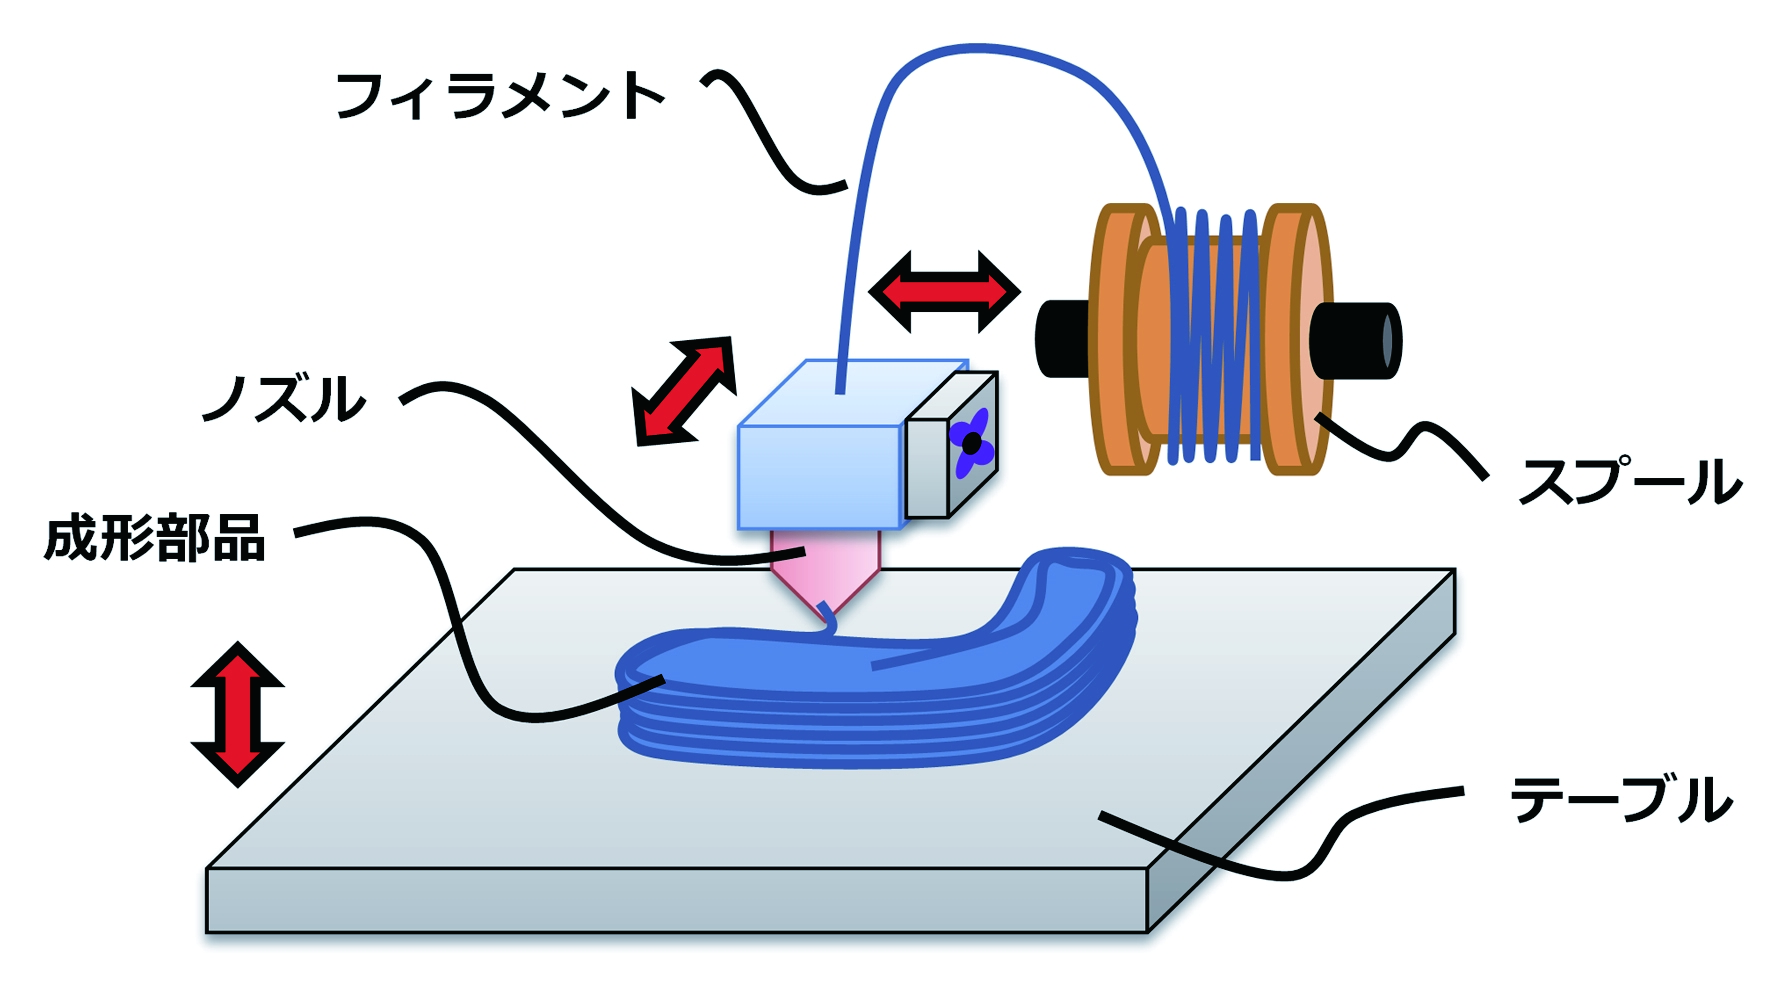
\includegraphics[width=300pt]{fig/fig22_cmyk.jpg}
\caption{熱溶解積層方式(FDM)の原理}
\label{fig22}
\end{figure}

\subsection{熱溶解積層方法の特徴}\label{ux71b1ux6eb6ux89e3ux7a4dux5c64ux65b9ux6cd5ux306eux7279ux5fb4}

熱溶解積層方法の3Dプリンタは下記のような特徴を持っています。

\subsubsection{長所}\label{ux9577ux6240}

\begin{itemize}
\tightlist
\item
  他方式の3Dプリンタより安価(本体・材料ともに)
\item
  使用できる材料の種類が豊富(材料種類・カラーが豊富)
\item
  樹脂を用いる3Dプリンタの中では、他の方式より比較的強い部品が作れる
\item
  3Dモデルだけで部品を作ることができる(2D図面が不要)
\end{itemize}

\subsubsection{短所}\label{ux77edux6240}

\begin{itemize}
\tightlist
\item
  原理的に寸法精度が切削加工ほど良くない(大凡0.1mmオーダー)
\item
  表面が荒い(側面に積層ピッチに応じた段差ができる)
\item
  衝撃や強い力が加わると積層面から剥がれることがある
\item
  成形時に部品に反りが発生することがある
\item
  大きな部品を作ると、時間がかかる(※製品によります)
\end{itemize}

\clearpage

\section{3Dプリンタの基本的な構造}\label{dux30d7ux30eaux30f3ux30bfux306eux57faux672cux7684ux306aux69cbux9020}

3Dプリンタの構造には大きく分けて以下の4つがあります。
図\ref{fig23}に構造別の長所・短所、製品例を挙げます。
因みにBOX型の製品例である「Replicator
2x(MakerBot社)」が私が持っている製品です。

\begin{itemize}
\tightlist
\item
  メンデル型
\item
  フレーム型
\item
  BOX型
\item
  ROSTOCK型
\end{itemize}

\begin{figure}[htbp]
\centering
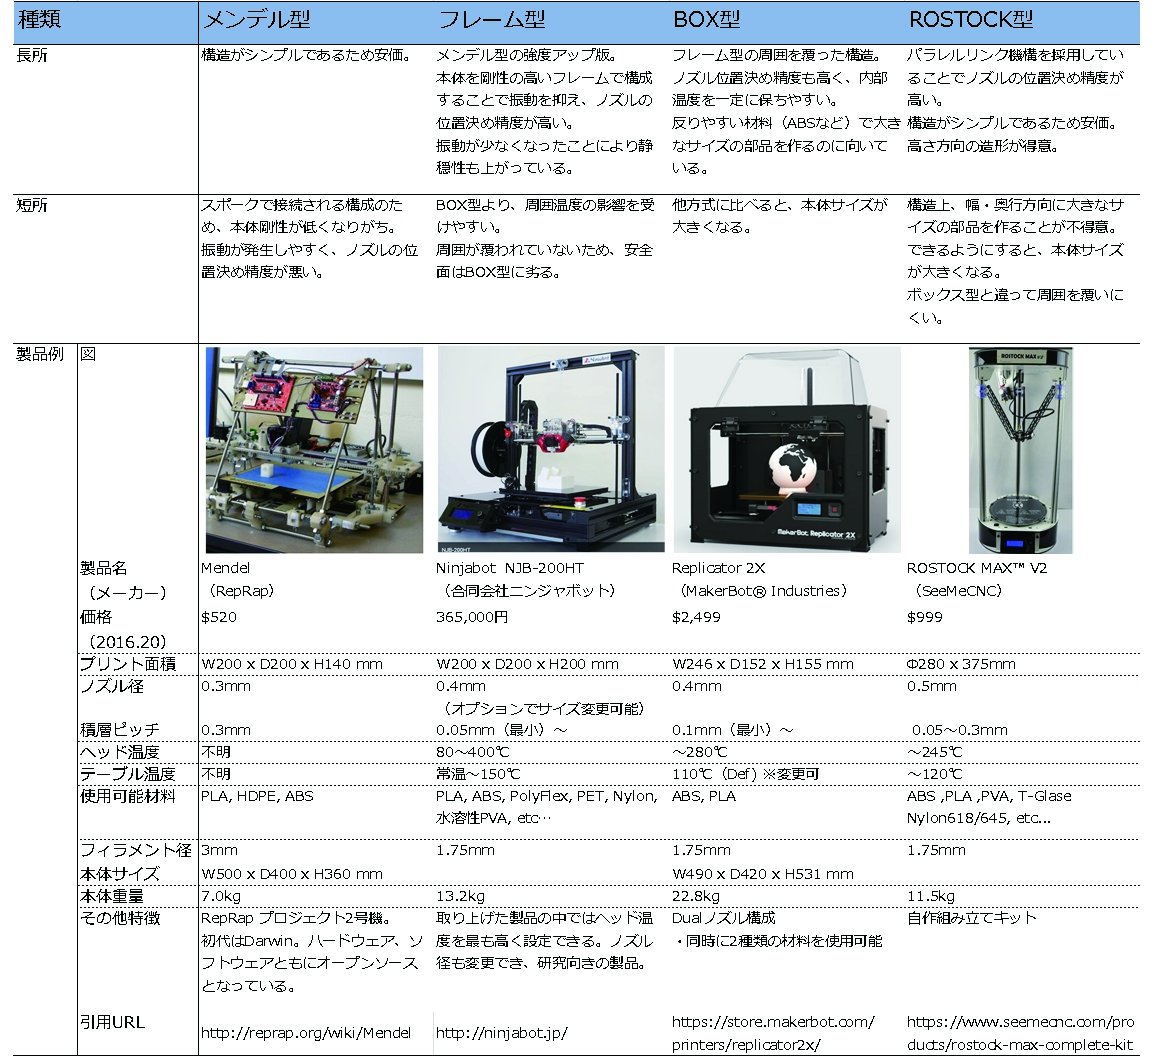
\includegraphics[width=380pt]{fig/fig23_cmyk.jpg}
\caption{3Dプリンタの構造}
\label{fig23}
\end{figure}

\section{3Dプリンタの選定}\label{dux30d7ux30eaux30f3ux30bfux306eux9078ux5b9a}

私が3Dプリンタを購入した当時(2013年)は選択肢が少なかったですが、2016年現在では非常に多くの製品が出ています。
前述したように3Dプリンタには短所も多いため、下記のような観点から自分に適した製品を選択する必要があります。

\begin{itemize}
\tightlist
\item
  使用材料・部品サイズ
\item
  寸法精度・外観
\item
  ユーザビリティ
\end{itemize}

\subsection{使用材料・部品サイズ}\label{ux4f7fux7528ux6750ux6599ux90e8ux54c1ux30b5ux30a4ux30ba}

3Dプリンタの代表的な造形材料はPLAとABSです。
特徴はFig.\ref{fig31}の通りです。

\begin{figure}[htbp]
\centering
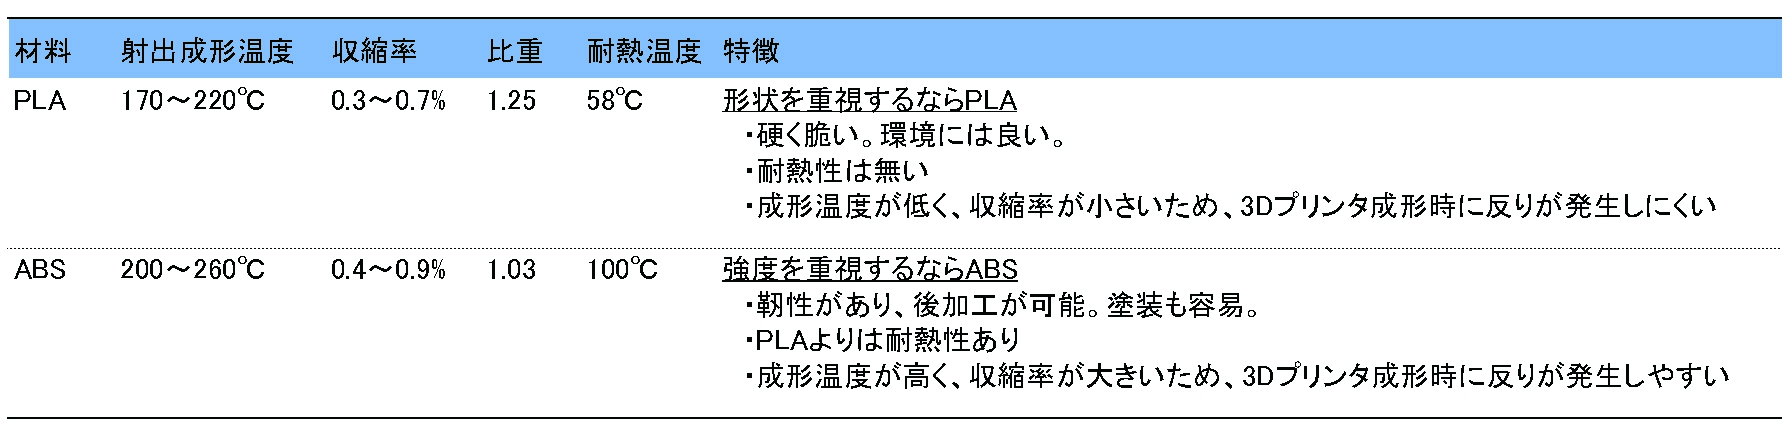
\includegraphics[width=360pt]{fig/fig31_cmyk.jpg}
\caption{代表的な造形材料と特徴}
\label{fig31}
\end{figure}

PLAよりもABSの方が成形が困難だと言われています。
ABSはPLAより収縮率が大きく、収縮力で最下層面とテーブルが剥がれ、部品に反りが出やすいためです。
(Fig.\ref{fig32})

\begin{figure}[htbp]
\centering
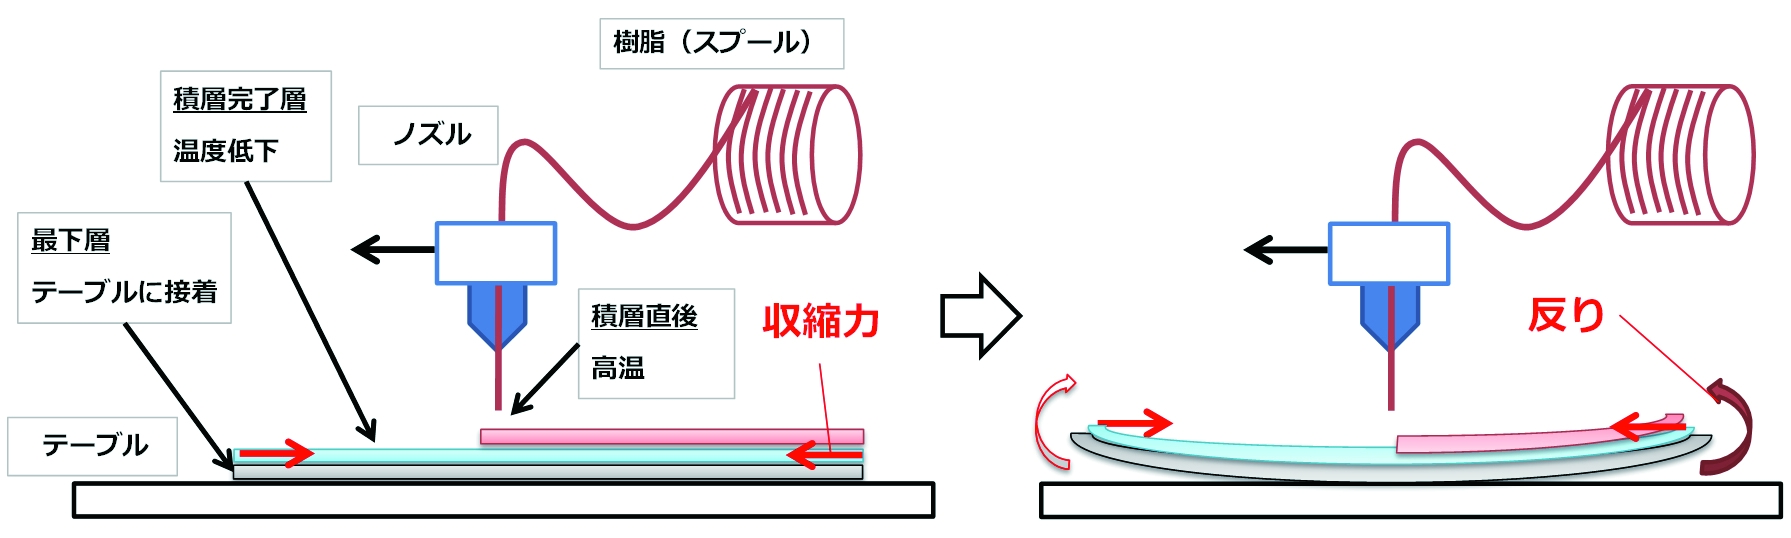
\includegraphics[width=380pt]{fig/fig32_cmyk.jpg}
\caption{反りの発生原理}
\label{fig32}
\end{figure}

よって、ABSをメインで使いたい場合は、ボックス型、かつ反り対策が入った製品がよいでしょう。
但し、部品サイズが小さければ(□100mm以下)、安価なフレーム型でも反りを出さずに部品を作ることが可能です。

\subsubsection{\texorpdfstring{製品例1:UP Plus(3D Systems
Inc.) ※Fig.\ref{fig28}
No.17}{製品例1:UP Plus(3D Systems Inc.) ※Fig. No.17}}\label{ux88fdux54c1ux4f8b1up-plus3d-systems-inc.fig.-no.17}

\begin{itemize}
\tightlist
\item
  □140mmまで対応したフレーム型3Dプリンタで、ABSに対応しています。
\item
  テーブル非加熱式のフレーム型のため熱が逃げやすい構成ですが、
  テーブルに細かい穴が空いており最下層の樹脂が穴に食い込むことで剥がれにくい対策を取っています。
\end{itemize}

因みに、同メーカから2016年に「UP BOX+」という後継機が出ています。
プリントサイズは□120mmまでと小さくなっていますが、ボックス型のため、反りがでにくそうです。

□150mmを大きく超えるサイズの部品をABSで作る場合には、以下のような積極的に反りを抑制する工夫が入った製品をお勧めします。

\subsubsection{\texorpdfstring{製品例2:Zortrax M200(Zortrax)
 ※Fig.\ref{fig26}
No.10}{製品例2:Zortrax M200(Zortrax)  ※Fig. No.10}}\label{ux88fdux54c1ux4f8b2zortrax-m200zortrax-fig.-no.10}

\begin{itemize}
\tightlist
\item
  □200mmまで対応したボックス型3Dプリンタで、ABSに対応しています。
\item
  テーブル加熱式、かつボックス型のため熱が逃げにくい構成となっており、成形安定性に定評があります。
\end{itemize}

\subsubsection{フィラメント径}\label{ux30d5ux30a3ux30e9ux30e1ux30f3ux30c8ux5f84}

フィラメント径はΦ1.75,
Φ3mmの2種類がありますが、現在はΦ1.75mmが主流です。

フィラメントは非正規品も多く出ていますが、品質が悪いものもあるのでご注意ください。
1kg3000円程度とコストは魅力的ですが、問題が発生することも多々あります。
例えば、フィラメントの線径にばらつきがあると部品形状にもムラができたり、最悪ノズルが詰まって成形に失敗することもあります。

\subsubsection{特殊フィラメント}\label{ux7279ux6b8aux30d5ux30a3ux30e9ux30e1ux30f3ux30c8}

フィラメントの材料は以前はABSとPLAが主流でしたが、近年は様々な種類が出ています。

例えば、アメリカのNinjatekが開発したNijaflex\cite{ninjaflex}はポリウレタン系の熱可塑性エラストマー(TPE)という材料です。
プラスチックとゴムの中間材料であるため、弾性を有していることが特徴です(ショア硬さ:85A)。
1kg10000円程度で購入可能です(2016.12月現在)。

また、アメリカのMakerBoが開発した\}TOUGH
PLA\cite{tough-pla}はPLAであるものの、耐久性と衝撃強度に優れた材料になっています。
750g 6000円程度で購入可能です(2016.12月現在)。
物性値は下記の通りです。

\begin{itemize}
\tightlist
\item
  ABS\ldots{}\ldots{}曲げ強さ:79MPa, 曲げ弾性率:2669MPa
\item
  TOUGH PLA\ldots{}\ldots{}曲げ強さ:63MPa, 曲げ弾性率:2366MPa
\end{itemize}

その他にも、HIPS(耐衝撃性ポリスチレン)、NYL(ナイロン)、CON(導電性フィラメント)、PVA(水溶性ポリビニルアルコール)、ガラスフィラー入り材料、等々続々と使用できる材料が増えてきています。
樹脂を溶融させて再度固める、という点では射出成型と原理は同じなので、理屈では材料も同じものが使えます。
勿論ABSで発生する反りなどは3Dプリンタ特有の問題なので、既存の材料を3Dプリンタ向けにアレンジする必要はあるかと思いますが、今後も使える材料は増えていくと思われます。

尚、材料の溶融温度は樹脂材料によって決まりますので、ノズルの最高温度が高く、かつ自由に設定できる製品であるほど使用できる材料の幅が広くなると思います。
将来に材料が増えることに期待して、ノズル温度を高くできる製品を選択するというのもありかもしれませんね。

\subsubsection{\texorpdfstring{製品例3:Ninjabot
NJB-200HT(合同株式会社ニンジャボット)
 ※Fig.\ref{fig23}}{製品例3:Ninjabot NJB-200HT(合同株式会社ニンジャボット)  ※Fig.}}\label{ux88fdux54c1ux4f8b3ninjabot-njb-200htux5408ux540cux682aux5f0fux4f1aux793eux30cbux30f3ux30b8ux30e3ux30dcux30c3ux30c8-fig.}

\begin{itemize}
\tightlist
\item
  樹脂の可能性そのものを研究する目的で開発されたフレーム型3Dプリンタです。
\item
  テーブルは150℃まで加熱でき、ノズルも、80~400℃と低温から高温までカバーしています。
\end{itemize}

\subsection{寸法精度・外観}\label{ux5bf8ux6cd5ux7cbeux5ea6ux5916ux89b3}

寸法精度・外観に影響を与える項目は前述した「反り」の他に下記項目があげられます。

\begin{itemize}
\tightlist
\item
  位置決め精度
\item
  積層ピッチ
\end{itemize}

テーブル・ノズルの位置決め精度が寸法精度・外観へ影響を与えます。
また、剛性が弱い3Dプリンタでは振動による精度ばらつきが追加されます。

積層ピッチに関しては、小さいほど積層跡が目立たなくなり、外観は綺麗にできます。
但し、積層ピッチが小さいと成形に失敗しやすくなります。
樹脂を積層する際に、積層ピッチ以上に位置決めの精度がばらつくと、積層界面で樹脂が溶着しなくなるためです。

世の中の3Dプリンタを見ると、剛性が高く精度の高い3Dプリンタほど、積層ピッチが小さくなっています。

\subsection{ユーザビリティ}\label{ux30e6ux30fcux30b6ux30d3ux30eaux30c6ux30a3}

3Dプリンタはいまだ発展途上の製品のため、ユーザが調整作業やメンテナンスをすることが多いです。
3Dプリンタの構造や搭載されている機能によって、ユーザの負荷が変わりますので、選定の際にはユーザビリティを考慮する必要があるでしょう。

\subsubsection{ノズル高さ自動調整機能}\label{ux30ceux30baux30ebux9ad8ux3055ux81eaux52d5ux8abfux6574ux6a5fux80fd}

3Dプリンタの部品の出来具合を左右する要因の一つに、ノズルとテーブルの隙間量(Z方向)があります。
狭すぎるとノズルが樹脂が出てこずノズル詰まりの原因となります。
逆に広すぎると溶かした樹脂がテーブルに貼りつかず、成形失敗の原因となります。

自動調節機能が無い機種では、ノズル~テーブルの間に紙1枚(≒0.3mm)を通過させ、隙間量を手動調整することが多いです。
一方、ノズル高さ自動調整機能 (Fig.\ref{fig33}
(a))があると、成形前にノズル~テーブル間距離を自動で測定し、適切な隙間量に設定してくれます。

\subsubsection{テーブル傾き対応}\label{ux30c6ux30fcux30d6ux30ebux50beux304dux5bfeux5fdc}

ノズルの高さ自動調整機能を有した製品は数多くあっても、テーブルの傾きを物理的に補正する製品は殆どありません。
メカ機構が複雑になるからだと思われます。テーブル傾きの対応は製品ごとに様々です。

例えば、ノズル~テーブル間距離を測定する機能を持った製品の中には、テーブル上の4隅と中央の隙間を測定し、
どの程度調整すればよいか明示してくれるものもあります。この値をもとにユーザが手動調整します。

ノズル~テーブル高さの隙間測定機能を利用して、テーブル傾きに対応(Z軸オートキャリブレーション)した製品もあります。
最下層のサポート材の厚みで調整するタイプと、ノズルがテーブルの傾きに合わせて動くタイプ(Fig.\ref{fig33}
(b))、と2タイプあります。

\begin{figure}[htbp]
\centering
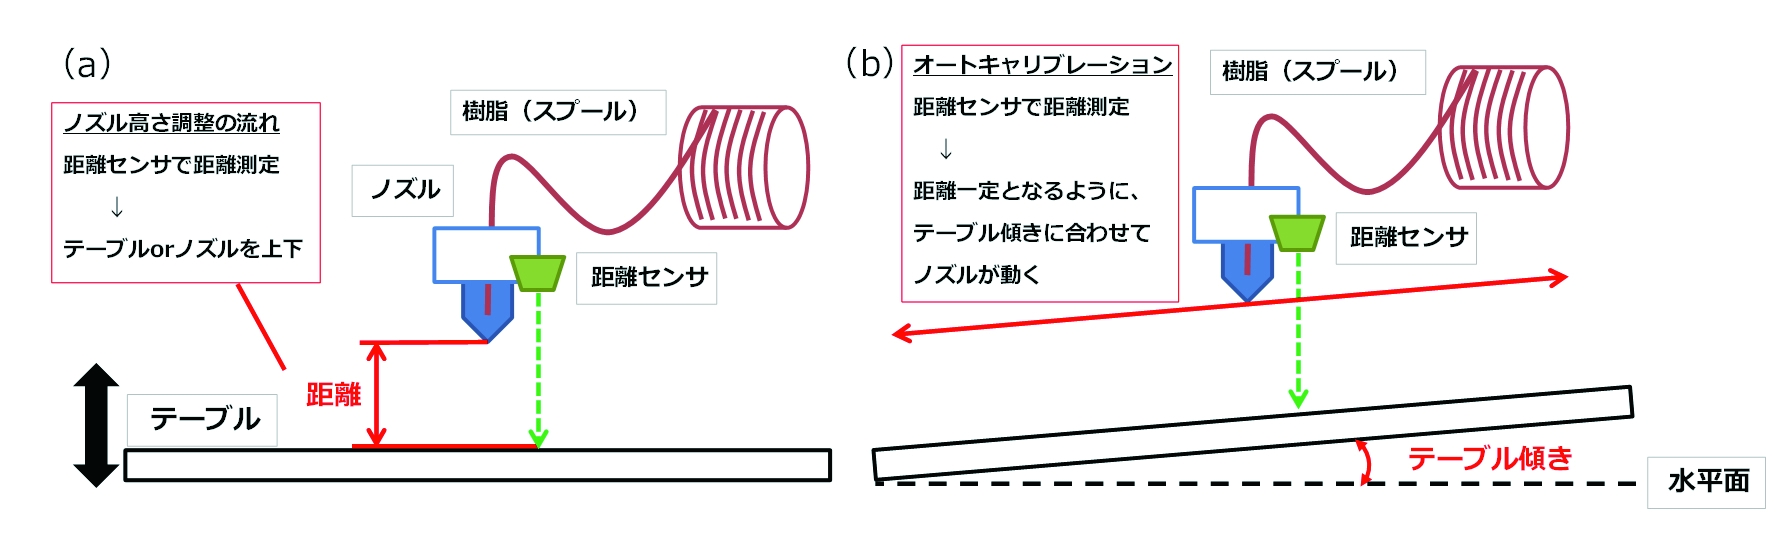
\includegraphics[width=380pt]{fig/fig33_cmyk.jpg}
\caption{ノズル高さ自動調節機能 / テーブル傾き対応}
\label{fig33}
\end{figure}

\subsection{コスト}\label{ux30b3ux30b9ux30c8}

コストには下記2つあります。

\begin{itemize}
\tightlist
\item
  本体価格
\item
  ランニングコスト
\end{itemize}

\subsubsection{本体価格}\label{ux672cux4f53ux4fa1ux683c}

本体価格は、Mendel型が最も安価です。
しかし、部品寸法精度や外観の観点から、あまりお勧めはしません。

2016年現在はそもそもMendel型のモデルは少なくなり、BOX型のモデルが充実してきています。
今後はROSTOCK型も増えていくでしょう。

10万~50万円くらいで幅広いラインナップが揃っていますので、
まずは最低限必要な機能を絞り、お財布と相談しながら候補を絞り込んでいくのがよいでしょう。

\subsubsection{ランニングコスト}\label{ux30e9ux30f3ux30cbux30f3ux30b0ux30b3ux30b9ux30c8}

ランニングコストに最も影響を与えるのが材料費用でしょう。

前述した通り、3Dプリンタは発展途上の製品なのでできるだけ純正フィラメントを使うことをお勧めします。
純正フィラメントの価格はメーカによって幅があります。
普通のABS樹脂ですと、純正品なら1kg 5000~6000円程度、非純正品なら1kg
3000円程度です。

1kgといっても、3Dプリンタの多くは部品の内側の充填率を下げて成形もできるので結構長持ちします。

尚、Cubeシリーズはやや高めの価格設定となっていますので、ランニングコストを気にされる方はご注意ください。

\section{3Dプリンタ一覧}\label{dux30d7ux30eaux30f3ux30bfux4e00ux89a7}

次ページから3Dプリンタの一覧を示します。

\clearpage

\begin{figure}[htbp]
\centering
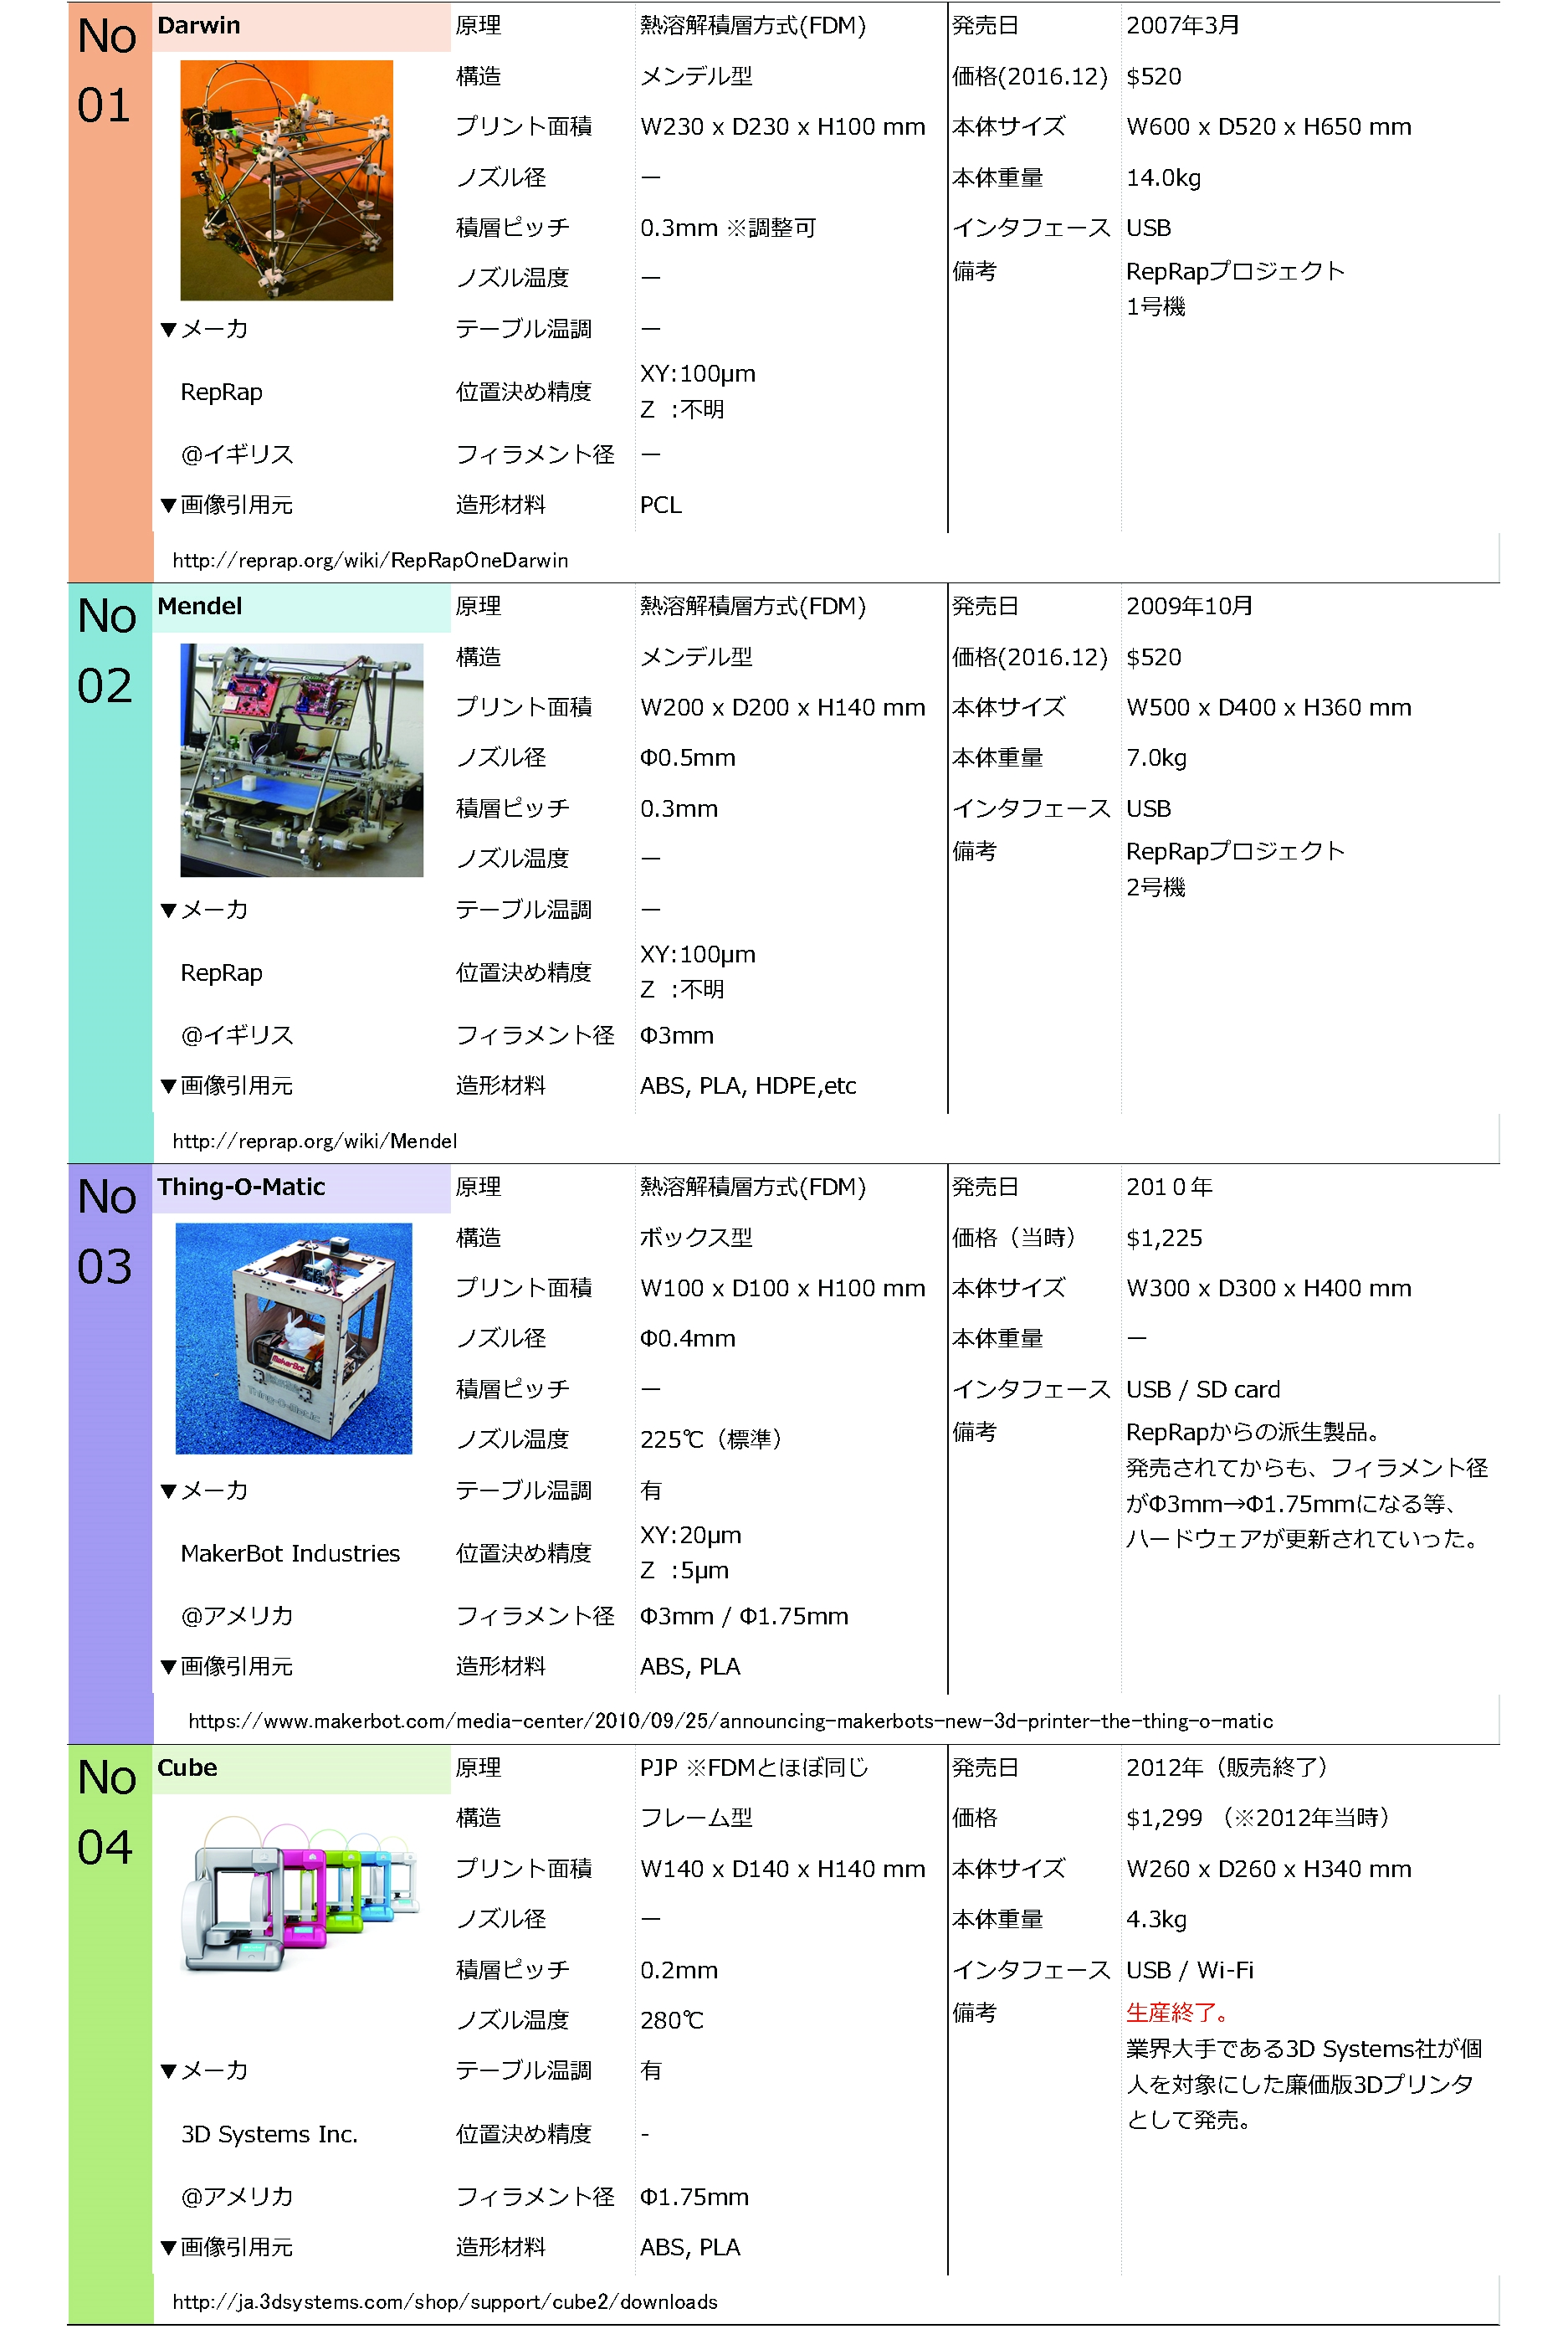
\includegraphics[width=380pt]{fig/fig24_cmyk.jpg}
\caption{3Dプリンタ一覧-1}
\label{fig24}
\end{figure}

\begin{figure}[htbp]
\centering
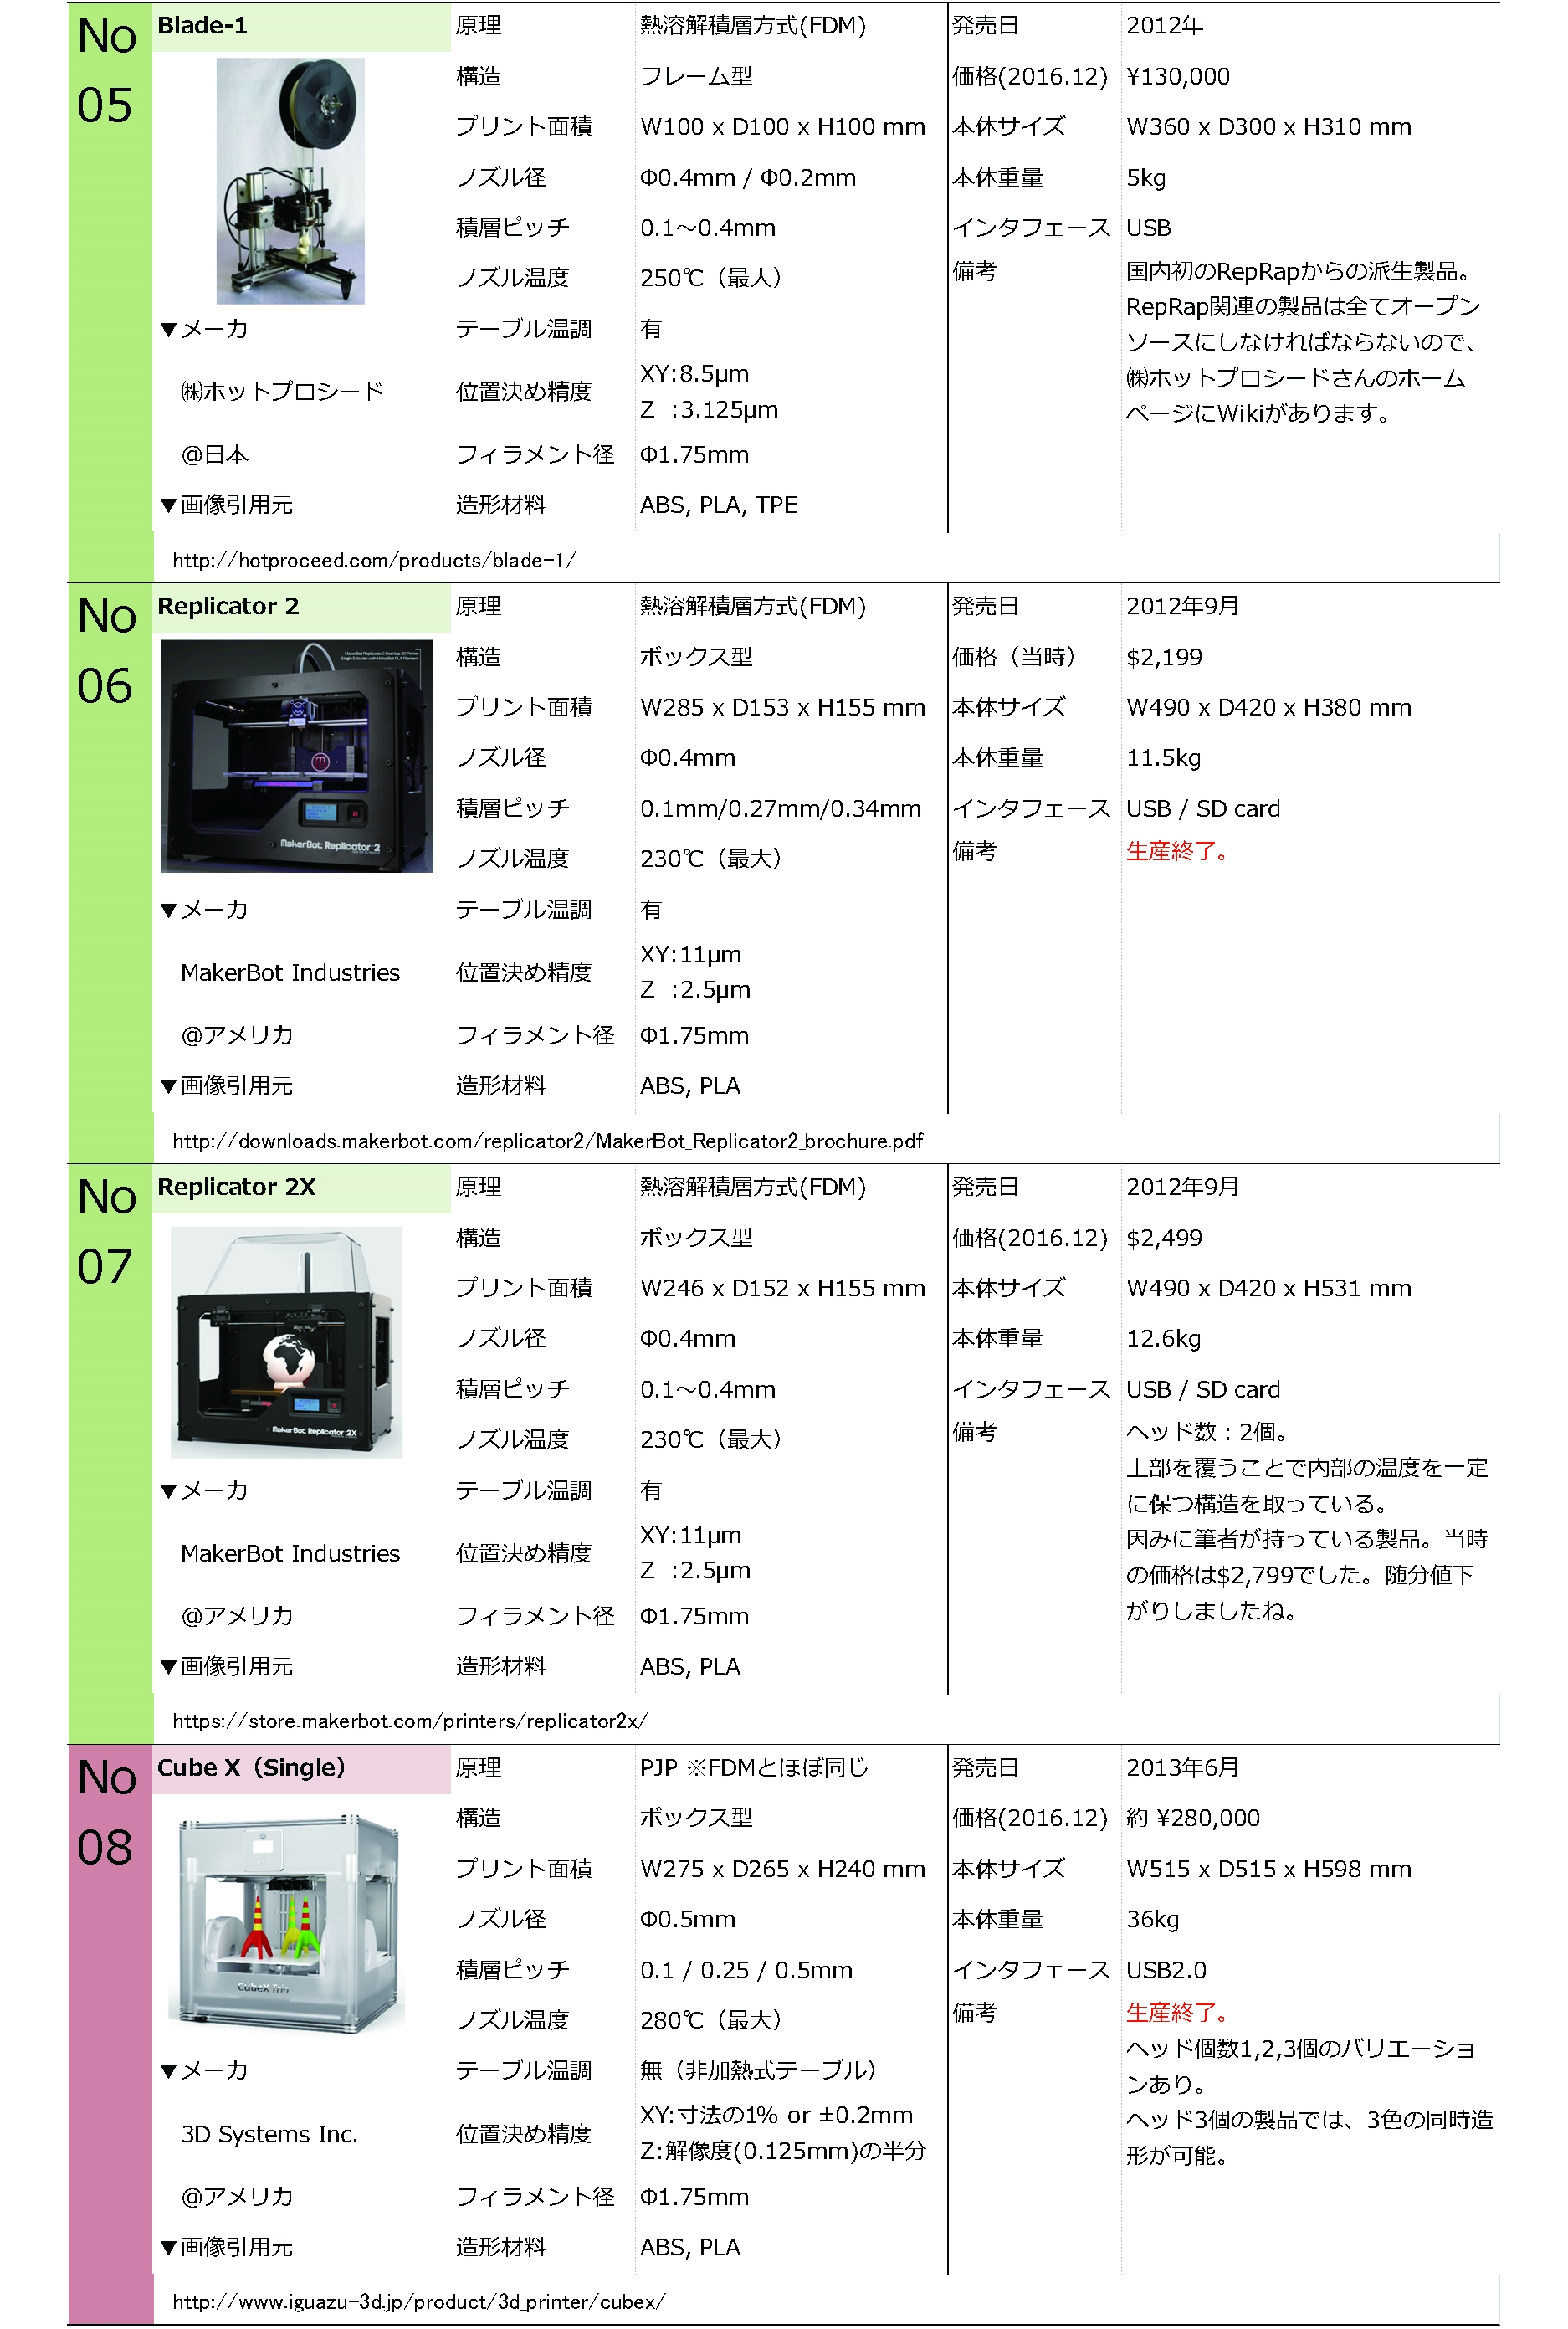
\includegraphics[width=380pt]{fig/fig25_cmyk.jpg}
\caption{3Dプリンタ一覧-2}
\label{fig25}
\end{figure}

\begin{figure}[htbp]
\centering
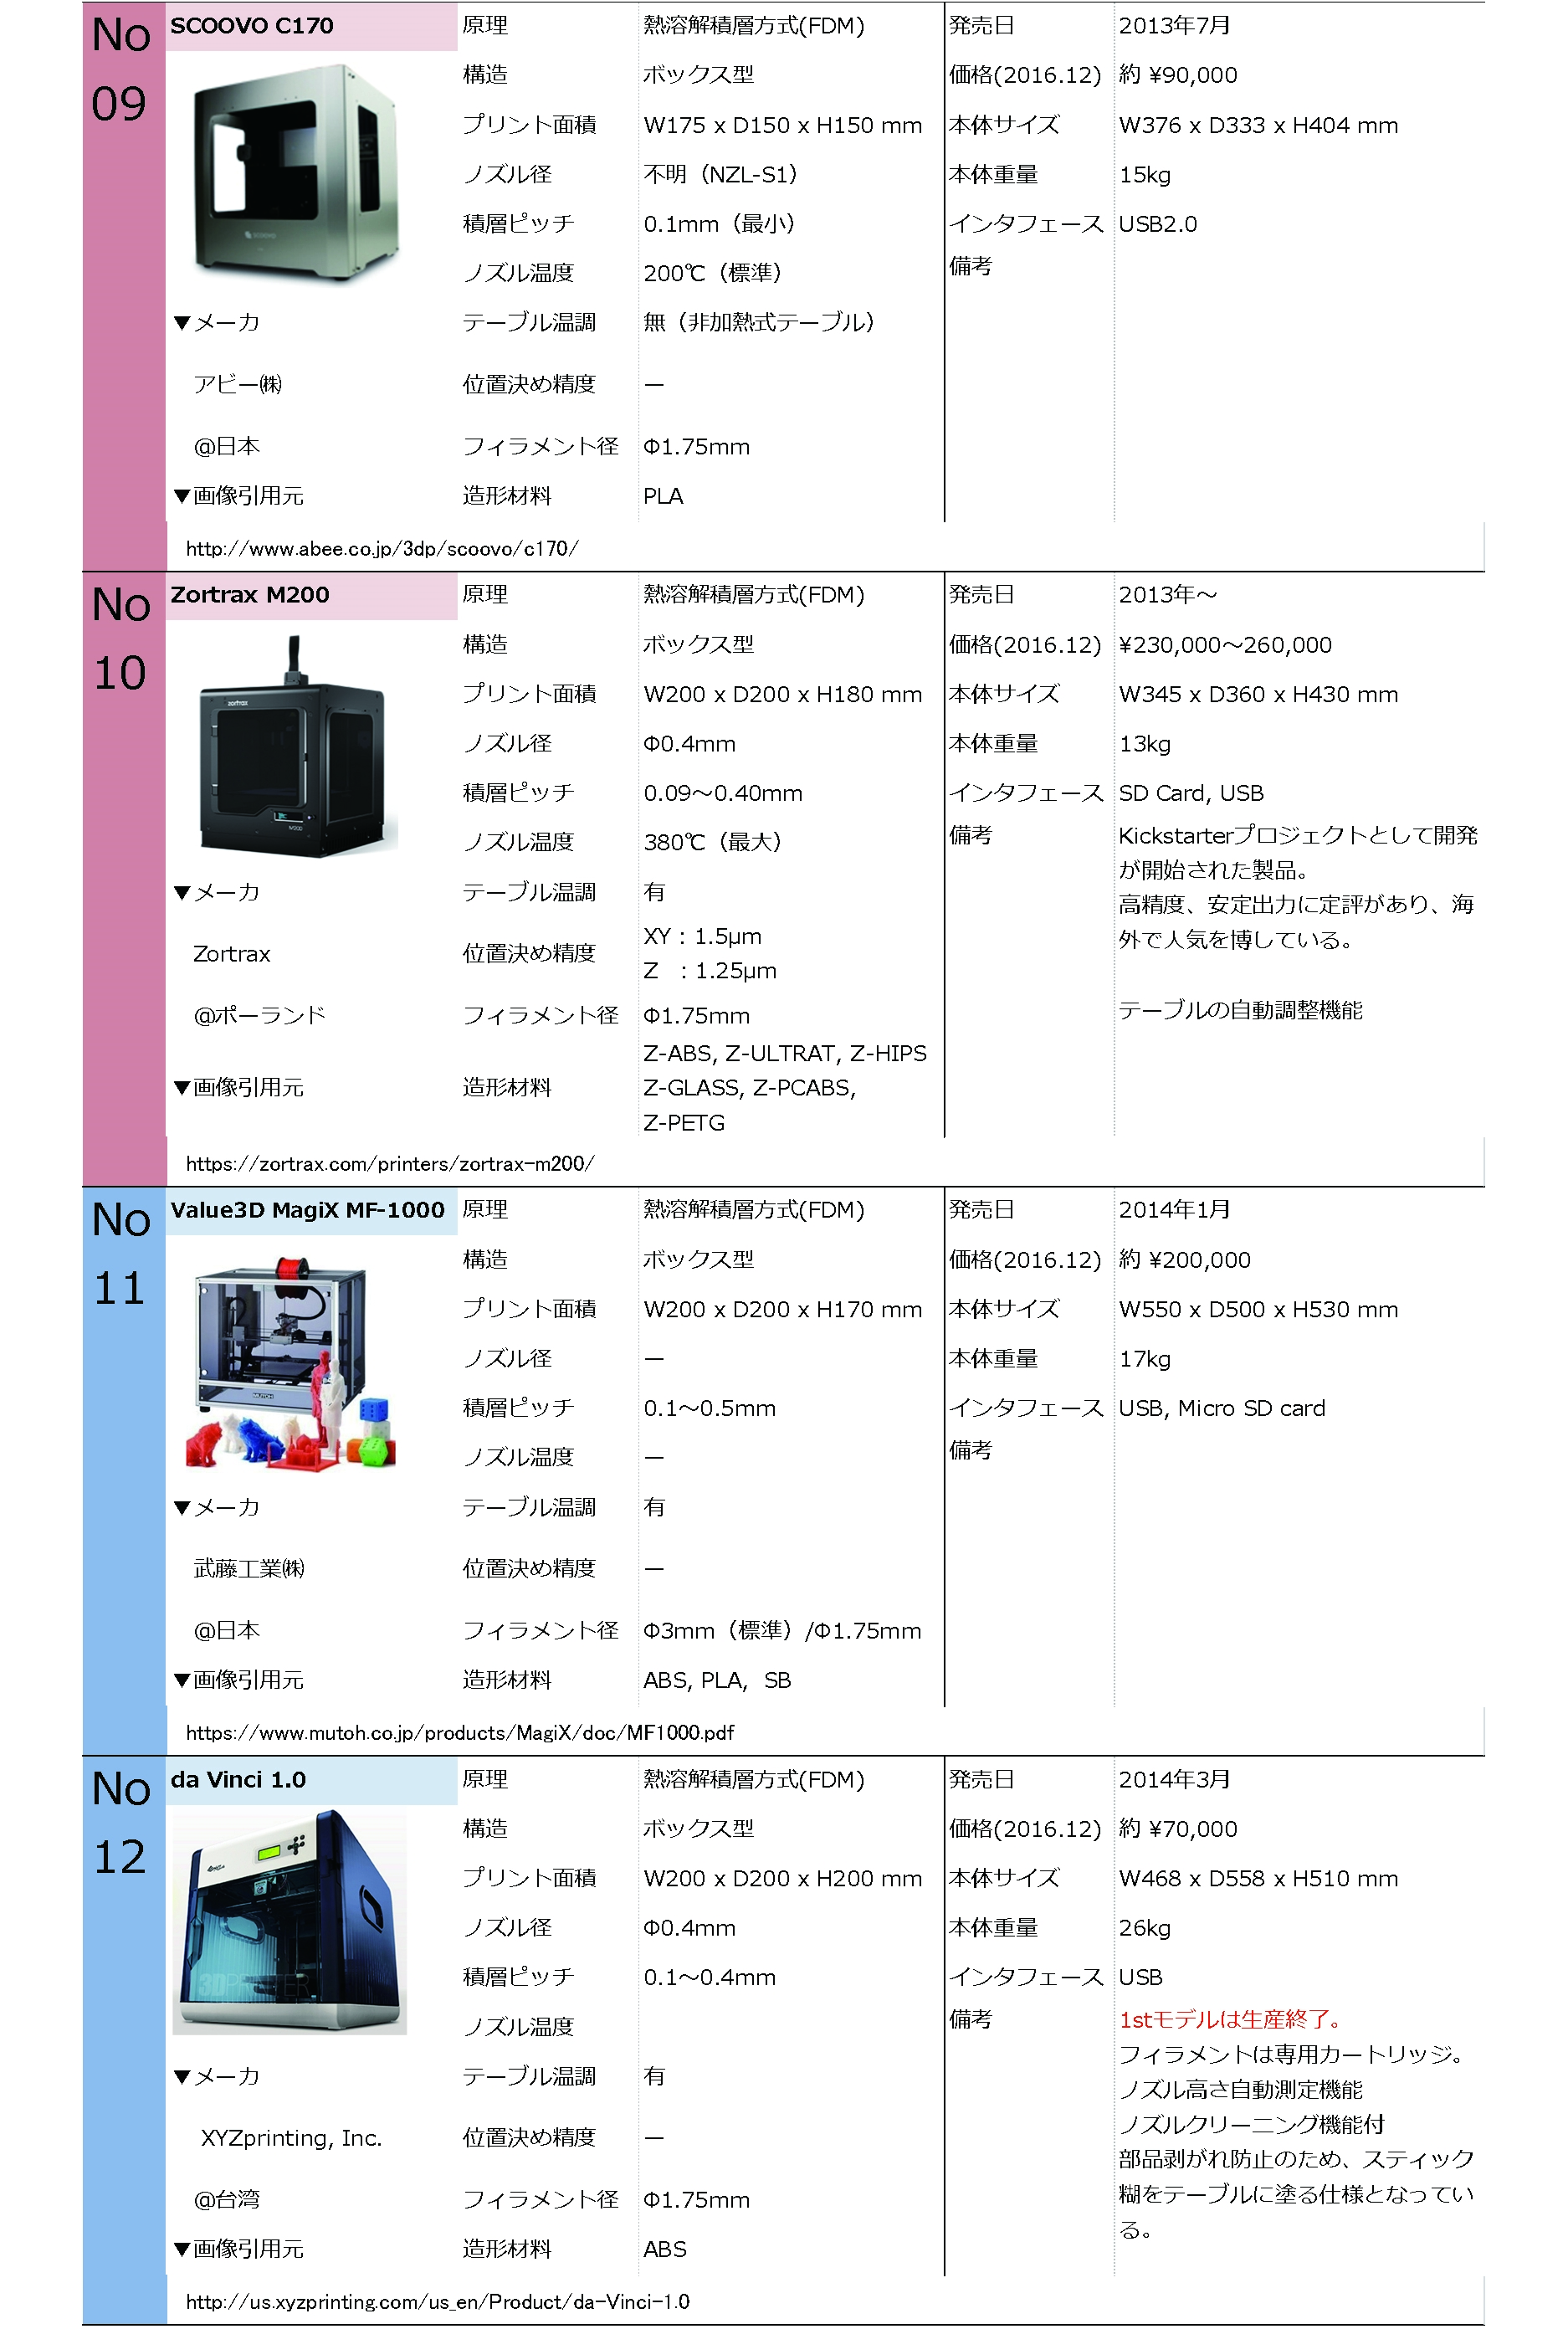
\includegraphics[width=380pt]{fig/fig26_cmyk.jpg}
\caption{3Dプリンタ一覧-3}
\label{fig26}
\end{figure}

\begin{figure}[htbp]
\centering
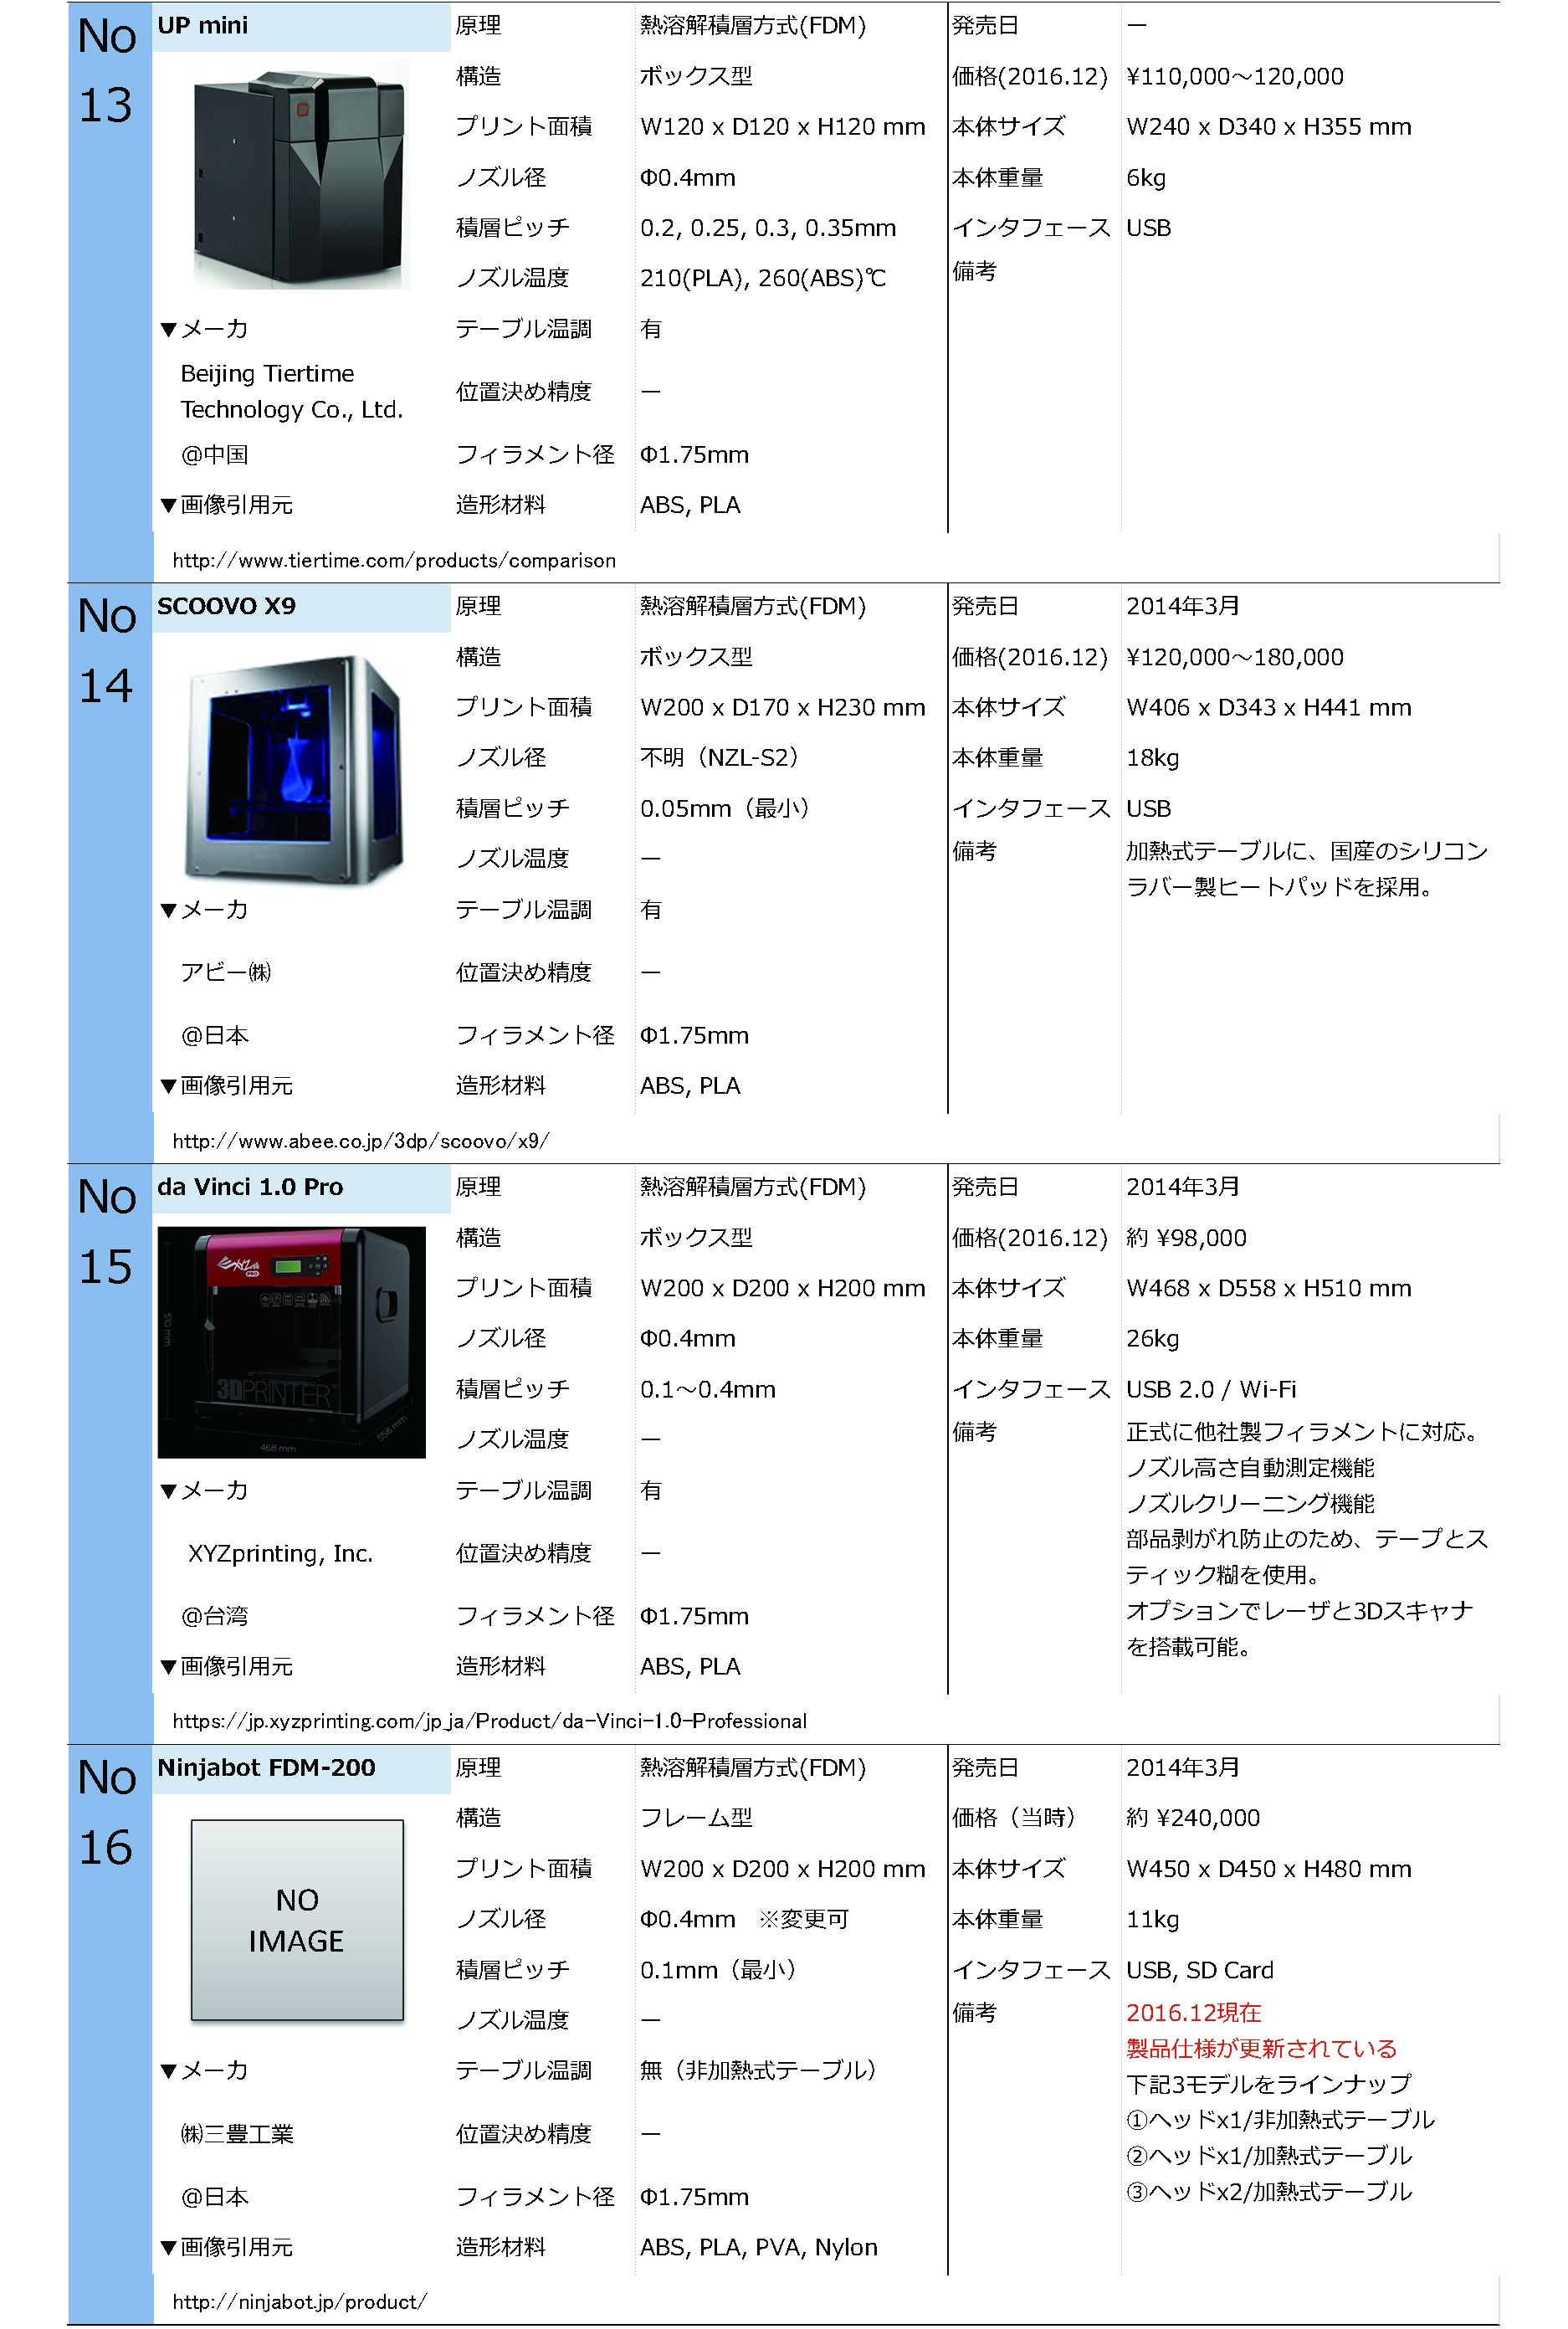
\includegraphics[width=380pt]{fig/fig27_cmyk.jpg}
\caption{3Dプリンタ一覧-4}
\label{fig27}
\end{figure}

\begin{figure}[htbp]
\centering
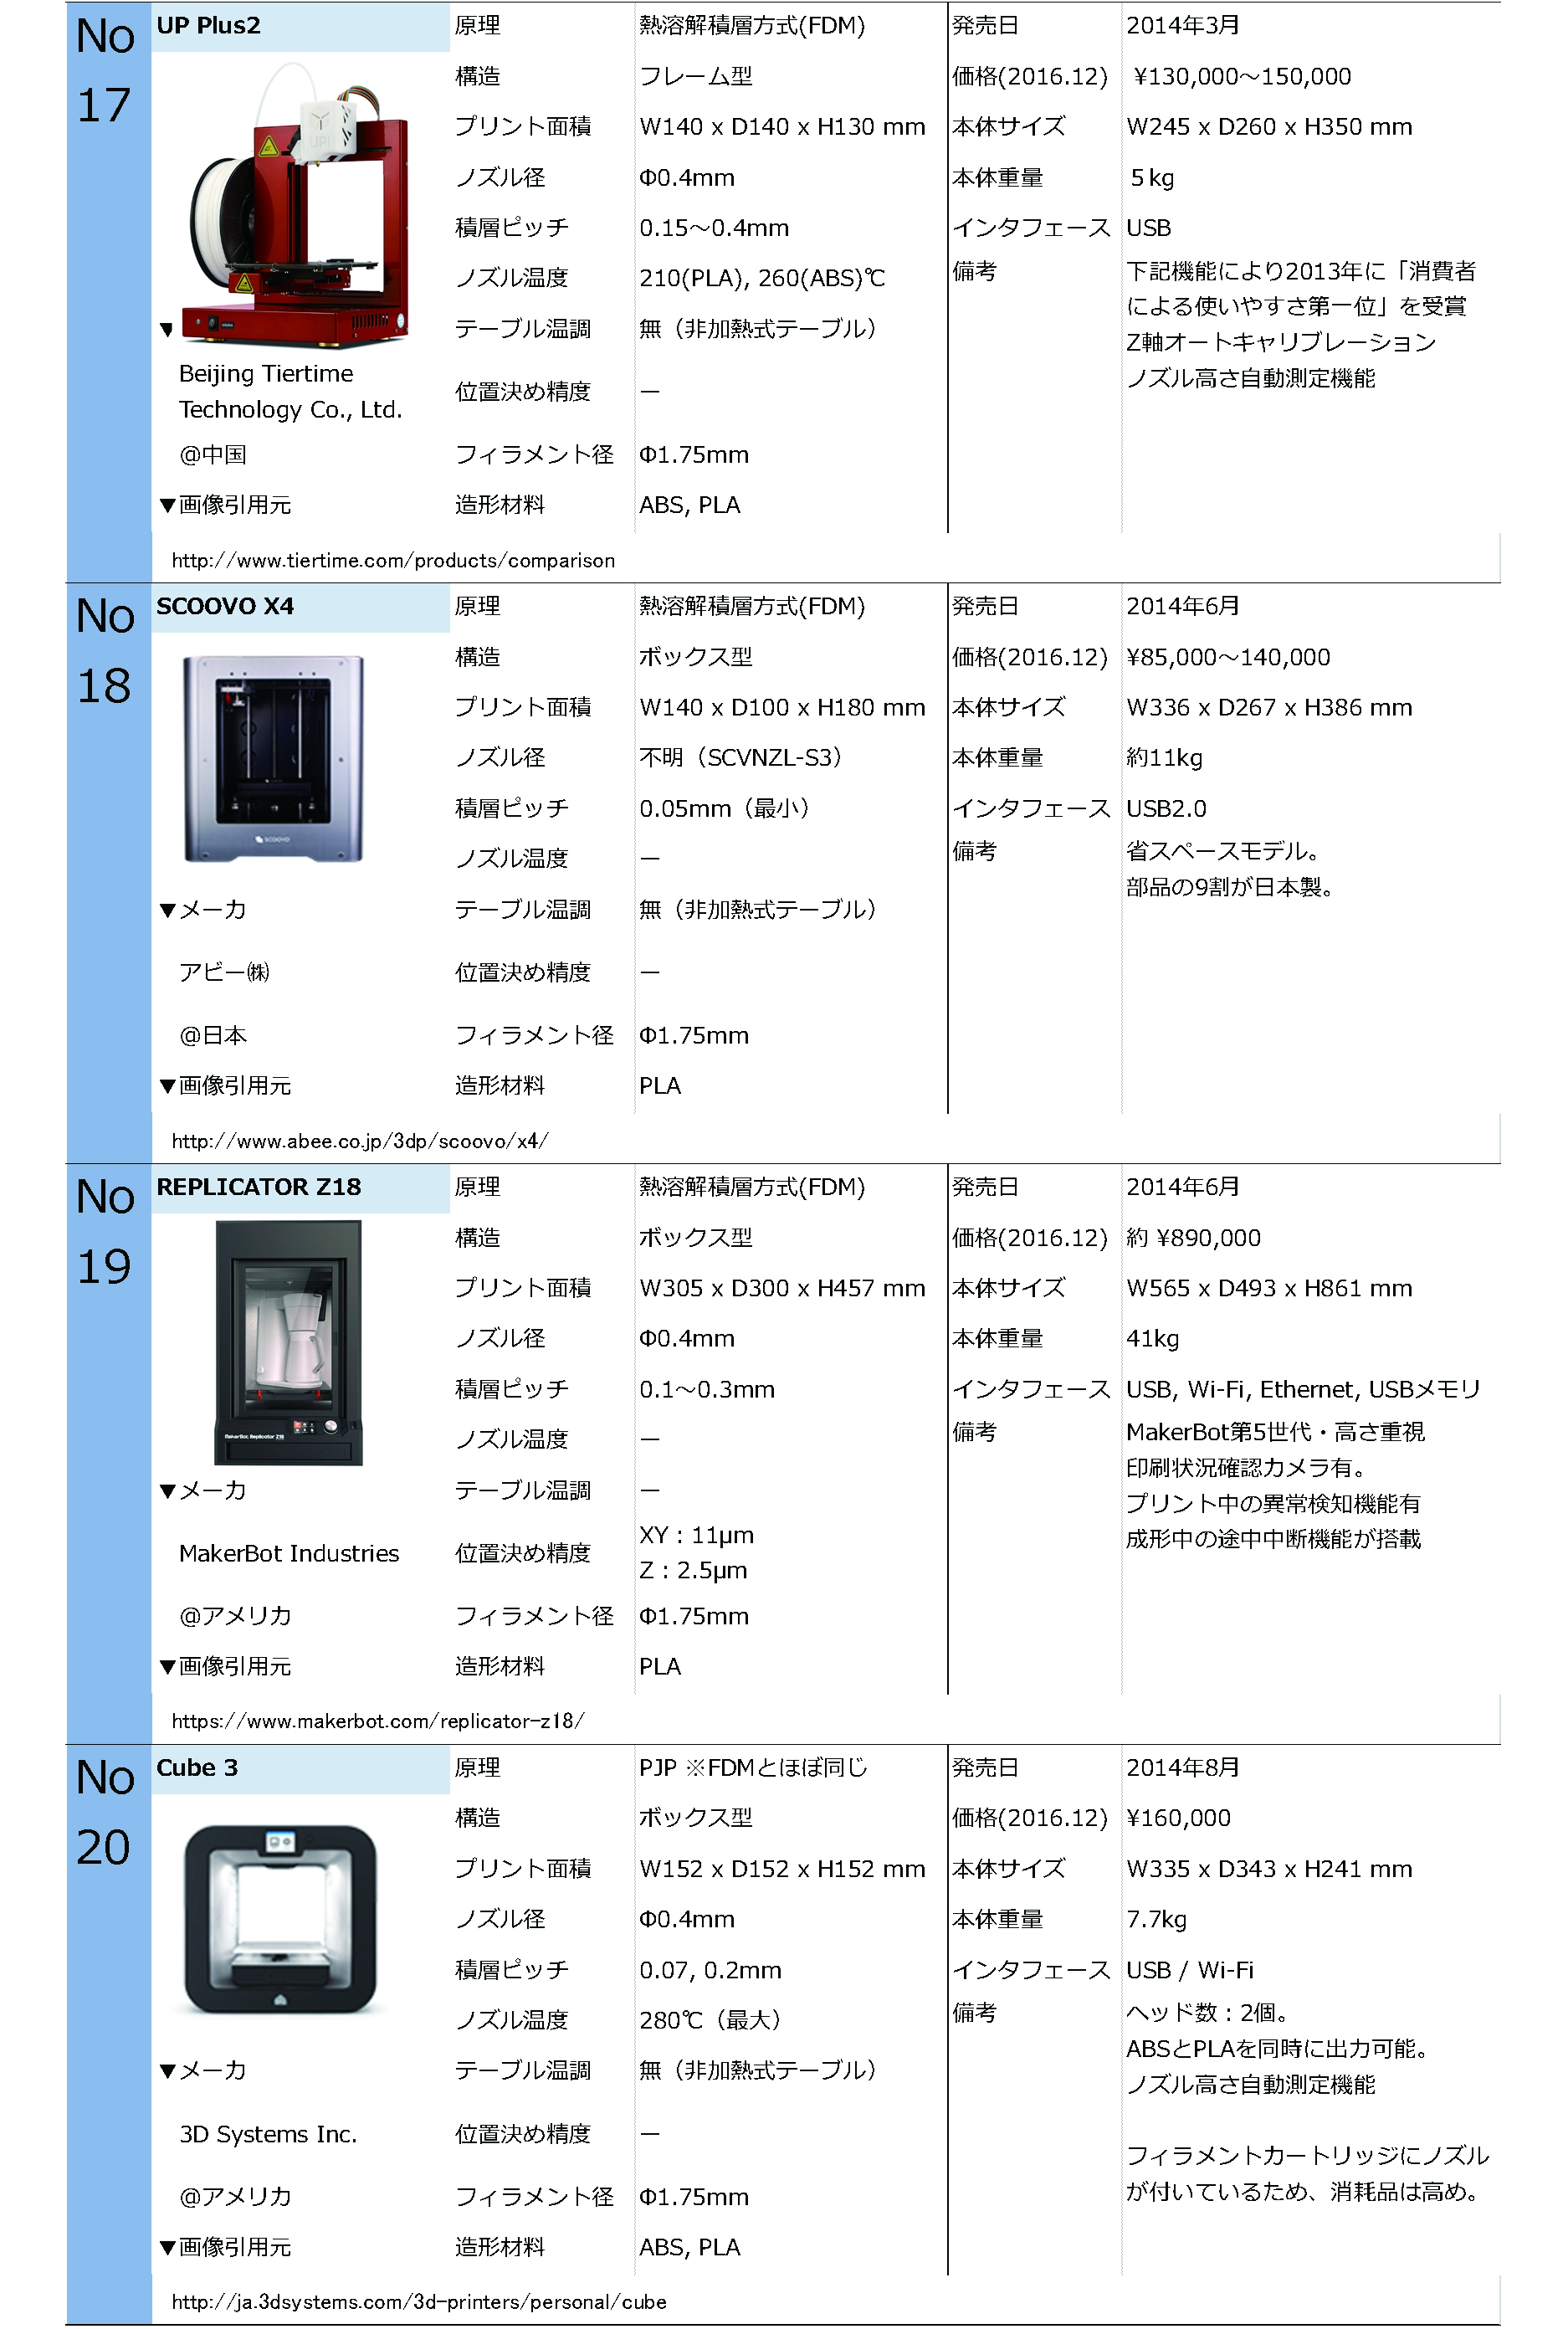
\includegraphics[width=380pt]{fig/fig28_cmyk.jpg}
\caption{3Dプリンタ一覧-5}
\label{fig28}
\end{figure}

\begin{figure}[htbp]
\centering
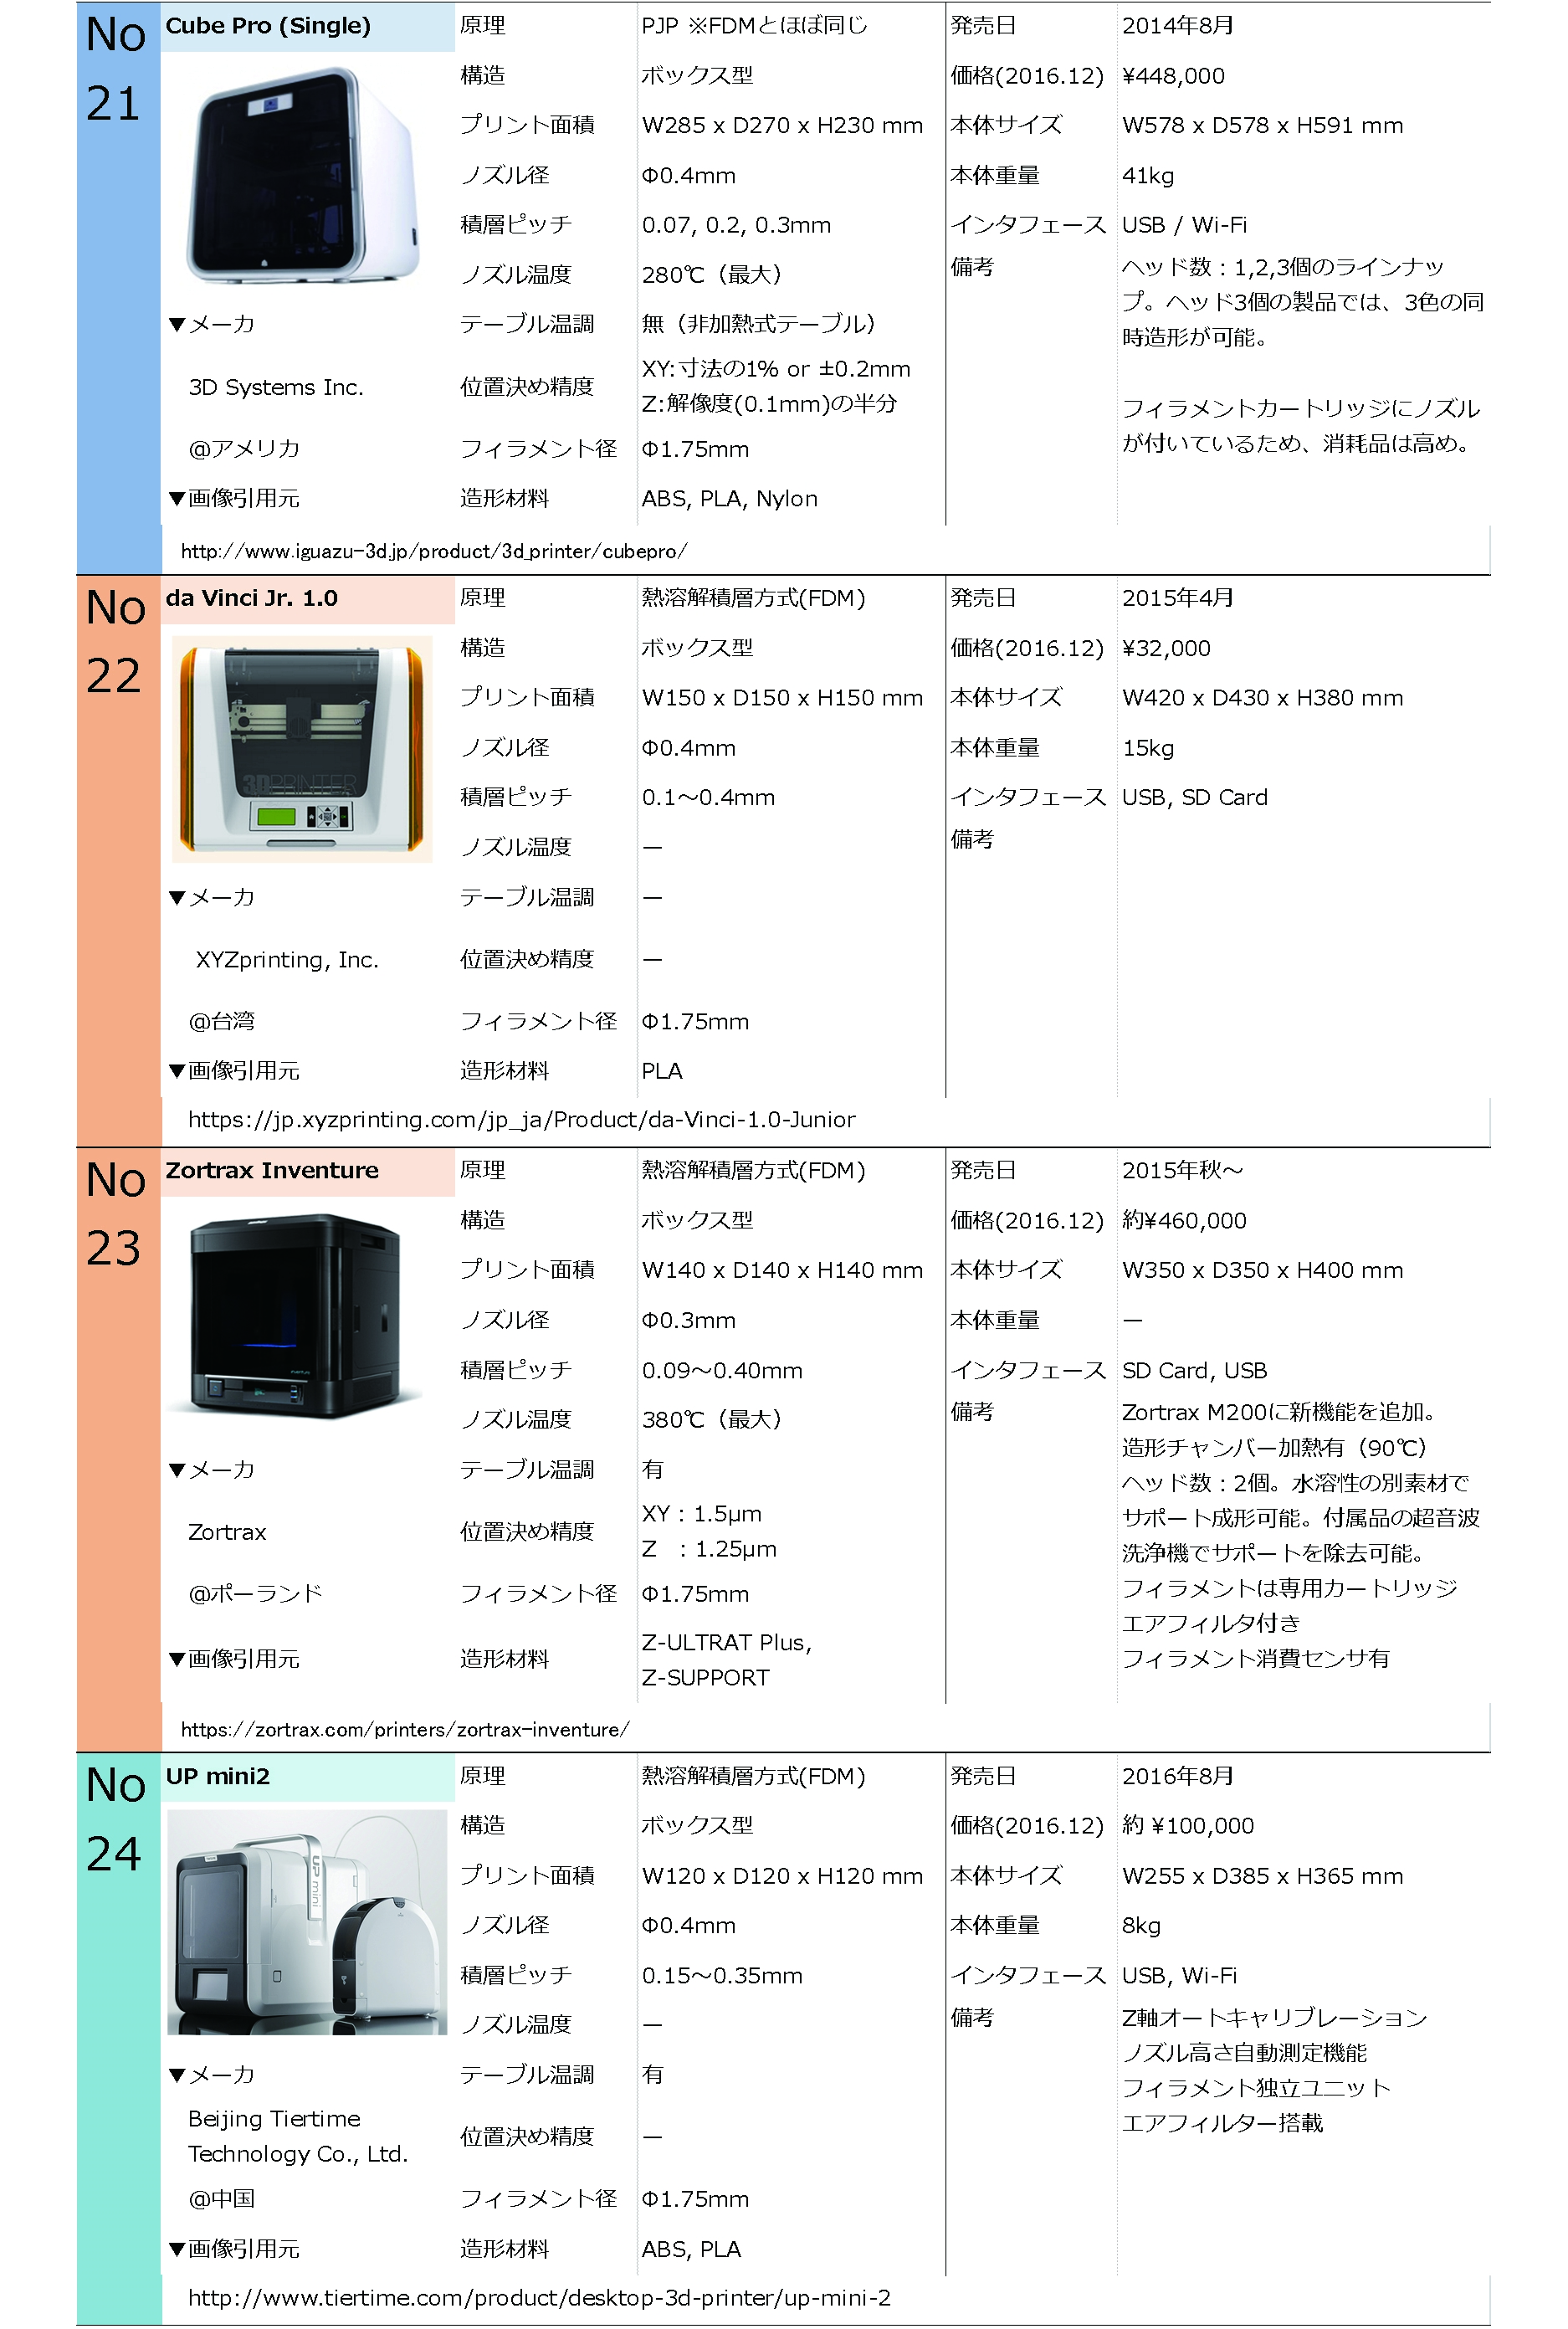
\includegraphics[width=380pt]{fig/fig29_cmyk.jpg}
\caption{3Dプリンタ一覧-6}
\label{fig29}
\end{figure}

\begin{figure}[htbp]
\centering
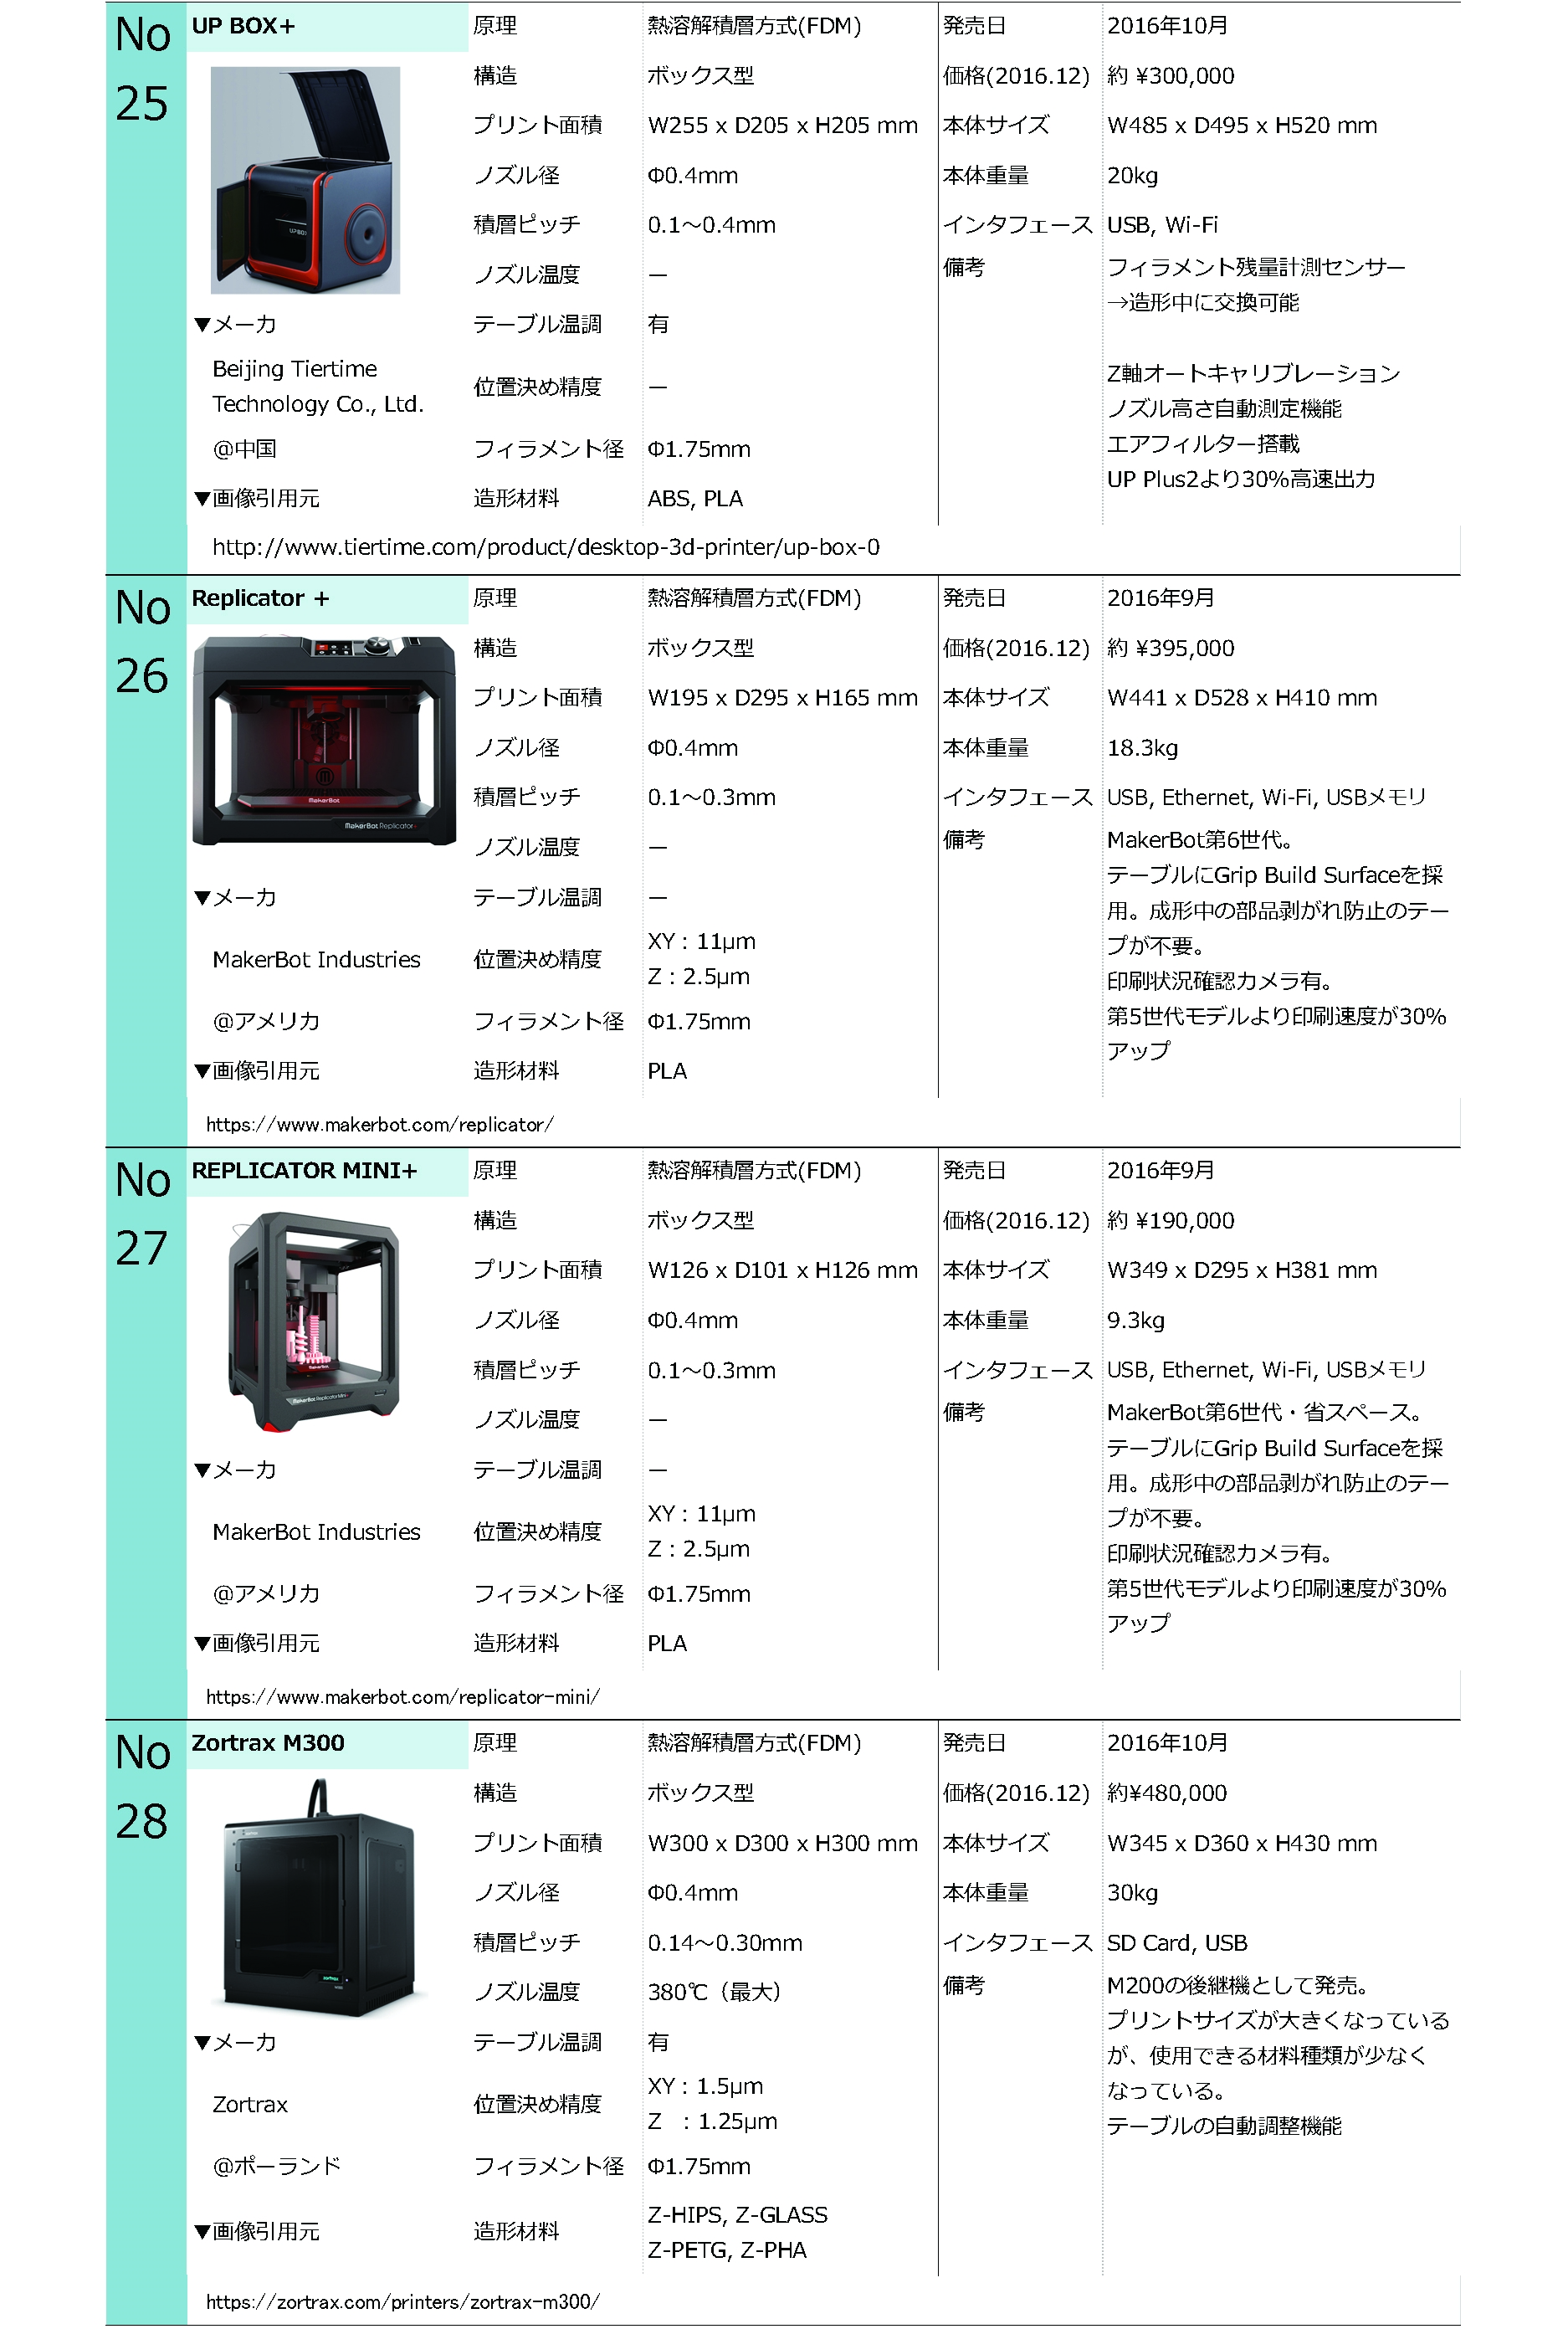
\includegraphics[width=380pt]{fig/fig30_cmyk.jpg}
\caption{3Dプリンタ一覧-7}
\label{fig30}
\end{figure}


\chapter{3Dプリンタでロボット設計}
\thispagestyle{fancy}
\section{ロボット競技大会の概要}\label{ux30edux30dcux30c3ux30c8ux7af6ux6280ux5927ux4f1aux306eux6982ux8981}

筆者は8月に川崎市で開催されるかわさきロボット競技大会というロボットコンテストに参加しています。
四角いリング上で2台のロボットに戦わせる対戦式の大会です。
(Fig.\ref{fig34})
ラジコンでよく使われるプロポでロボットを操作し、相手の機体をリング場外へ押し出すか、ダウンさせた後10カウント状態をキープすれば勝利となります。

\begin{figure}[htbp]
\centering
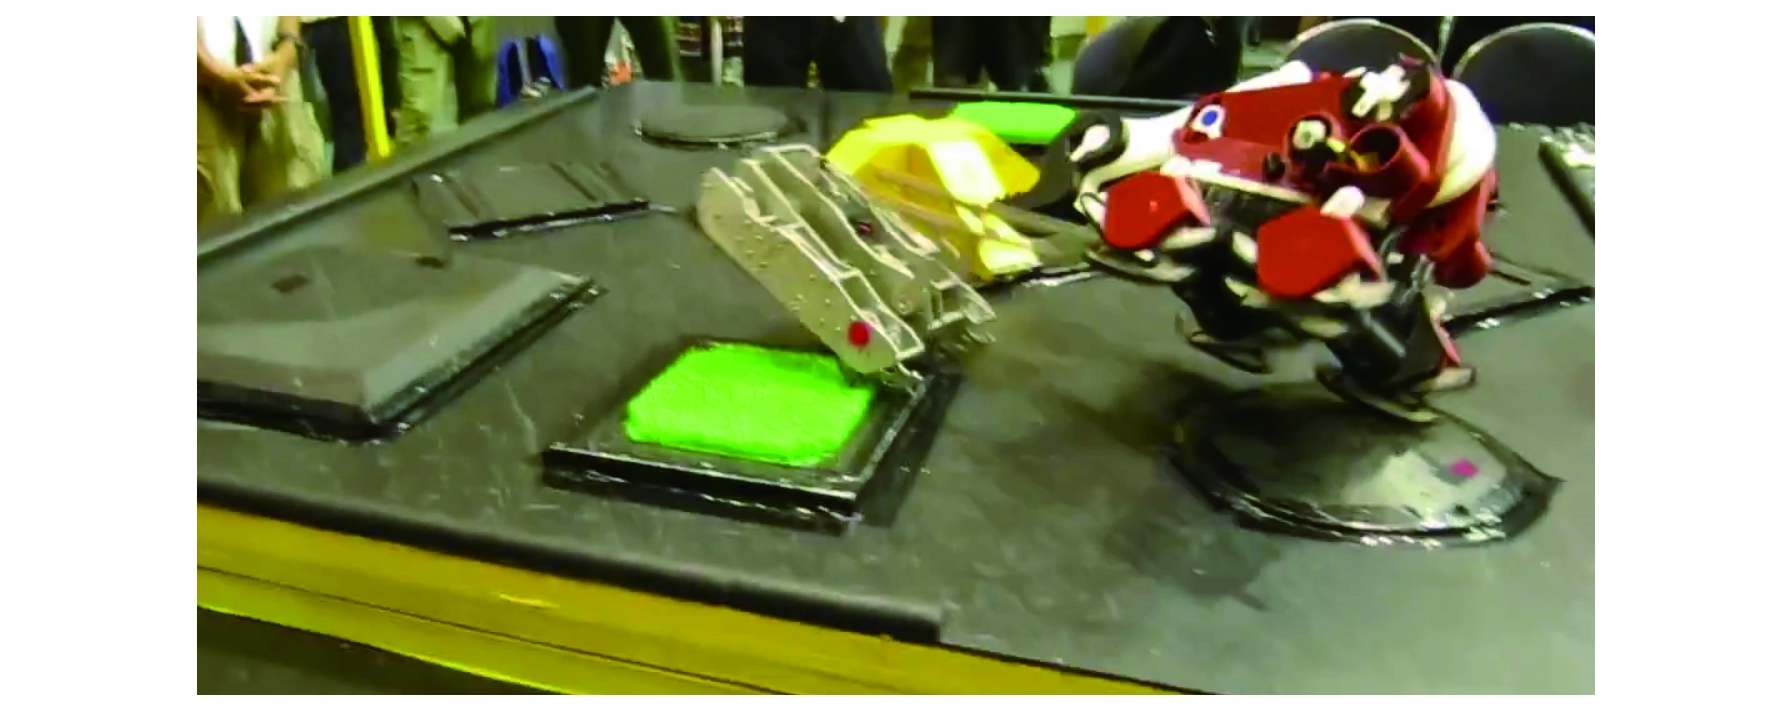
\includegraphics[width=380pt]{fig/fig34_cmyk.jpg}
\caption{かわさきロボット大会の様子}
\label{fig34}
\end{figure}

機体仕様には規定があります。以下に本体構成に関わる項目を列挙します。
以下のルールは2014年時に参加した時のものです。
現在は規則に幾つか変更が入っているため、詳細はかわさきロボット競技大会公式サイト\cite{kawasaki_public_HP}ご参照ください。

\begin{itemize}
\tightlist
\item
  サイズ制限:幅250mm×奥行350mm×高さ700mm(待機時)
\item
  重量制限:3500g以内
\item
  ロボットには、それぞれ1セット以上の脚機構、アーム機構が搭載されていること
\item
  脚部は、往復運動を行う部位を接地部として、リンク機構を用いて移動するように設計されていること
\item
  アーム部は、機構のみを用いて物体をアームで移動させることができ、大会が規定する揺動リンク機構を有し、高さ200mm地点を通過すること
\end{itemize}

\section{構想設計}\label{ux69cbux60f3ux8a2dux8a08}

\subsection{コンセプト}\label{ux30b3ux30f3ux30bbux30d7ux30c8}

2014年度のかわさきロボット競技大会では、筆者は下記のようにコンセプトを決めました。

\begin{enumerate}
\def\labelenumi{\arabic{enumi}.}
\tightlist
\item
  大会上、今までに無い機体を作りたい(新規性)
\item
  3Dプリンタでほぼ全ての部品を作る(見た目の分かりやすさ)
\item
  強度担保のため、極力シンプルな機構で構成する(実現性)
\end{enumerate}

今思い返すと3Dプリンタを活用することそのものが目的になっていました。
趣味だからこそできることですね。

\subsection{全体構成}\label{ux5168ux4f53ux69cbux6210}

上記コンセプトをもとにポンチ絵を描きました。(Fig.\ref{fig01})
細かい部分は考えず、全体の大きな構成を見通したいので、ざっくりした絵になっています。

個人的にはポンチ絵を描くツールはなんでもよいと考えています。
今回は、Excelのオートシェイプ機能を使って書きました。
手書きでもよいかと思います。

ポンチ絵を描きながら下記項目をまとめていきました。

\begin{itemize}
\tightlist
\item
  フレーム構造:底部フレームに側面フレームを取り付け、コの字型にすることで強度アップする。
\item
  脚部:4か所の脚部は全て共通化し、メンテナンス性を向上させる。取り付けは底部フレームとする。
\item
  アーム:相手機体と直接接触が多い個所なので、メンテナンス性(交換のしやすさ)が求められる。簡単に組み立て、分解ができるよう、側面フレームだけに取り付ける。
\item
  電装系:電装系は底部フレーム上に取り付ける。また、相手機体のアームが電装系に当たってしまうと動かなくなってしまうリスクがあるため、一旦組み立ててしまえば外からはアクセスできなようにする。
   \\

  \begin{figure}[htbp]
  \centering
  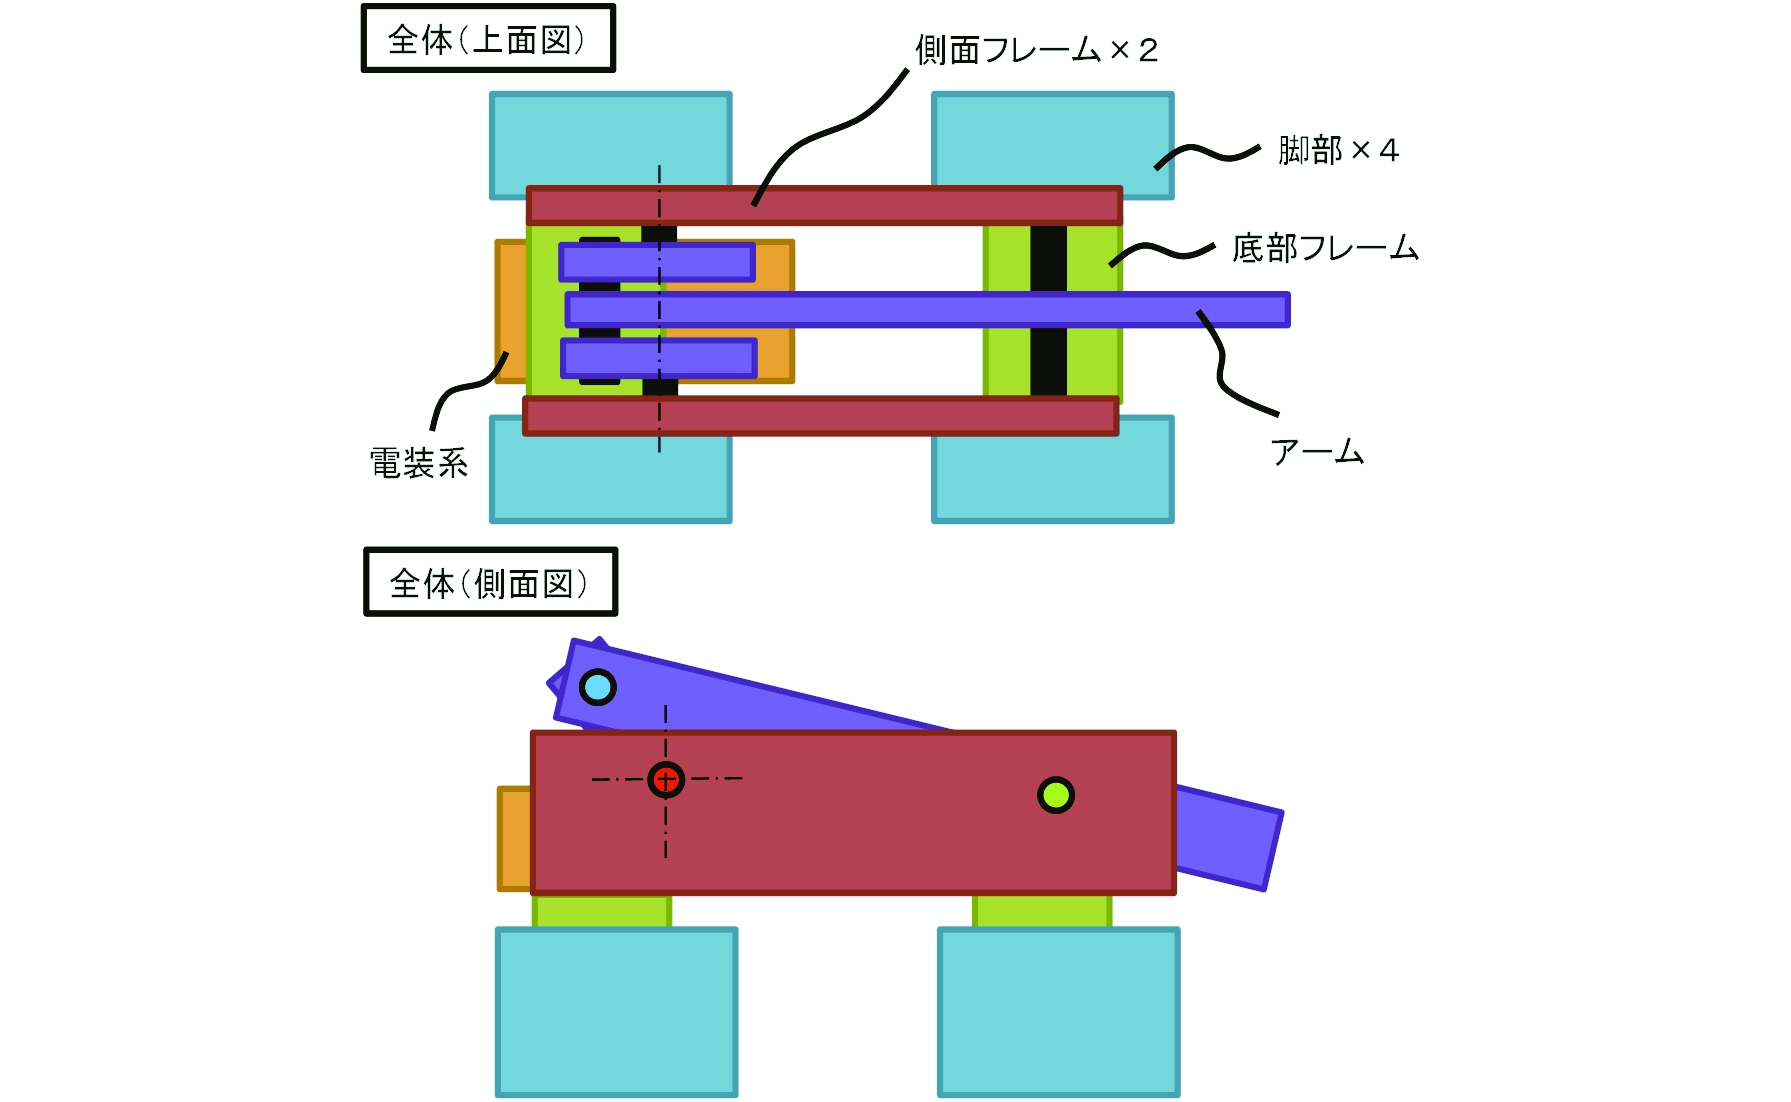
\includegraphics[width=380pt]{fig/fig01_cmyk.jpg}
  \caption{全体構成 ポンチ絵}
  \label{fig01}
  \end{figure}
\end{itemize}

\subsection{脚構成}\label{ux811aux69cbux6210}

\begin{itemize}
\tightlist
\item
  リンク機構:シンプルなスライダリンク機構を採用し、低強度な部品でも問題が出ないようにする
\item
  脚厚み:足先は走行時の衝撃が加わるため、なるべく厚くして強度アップを狙う
\item
  脚個数:一つの脚部には足を3枚用いる。足は位相を120°ずつずらして並列に配置することで、常に足先を地面に接地させる。これによりロボットの上下振動が抑えられ、走破性が良化する
\end{itemize}

\begin{figure}[htbp]
\centering
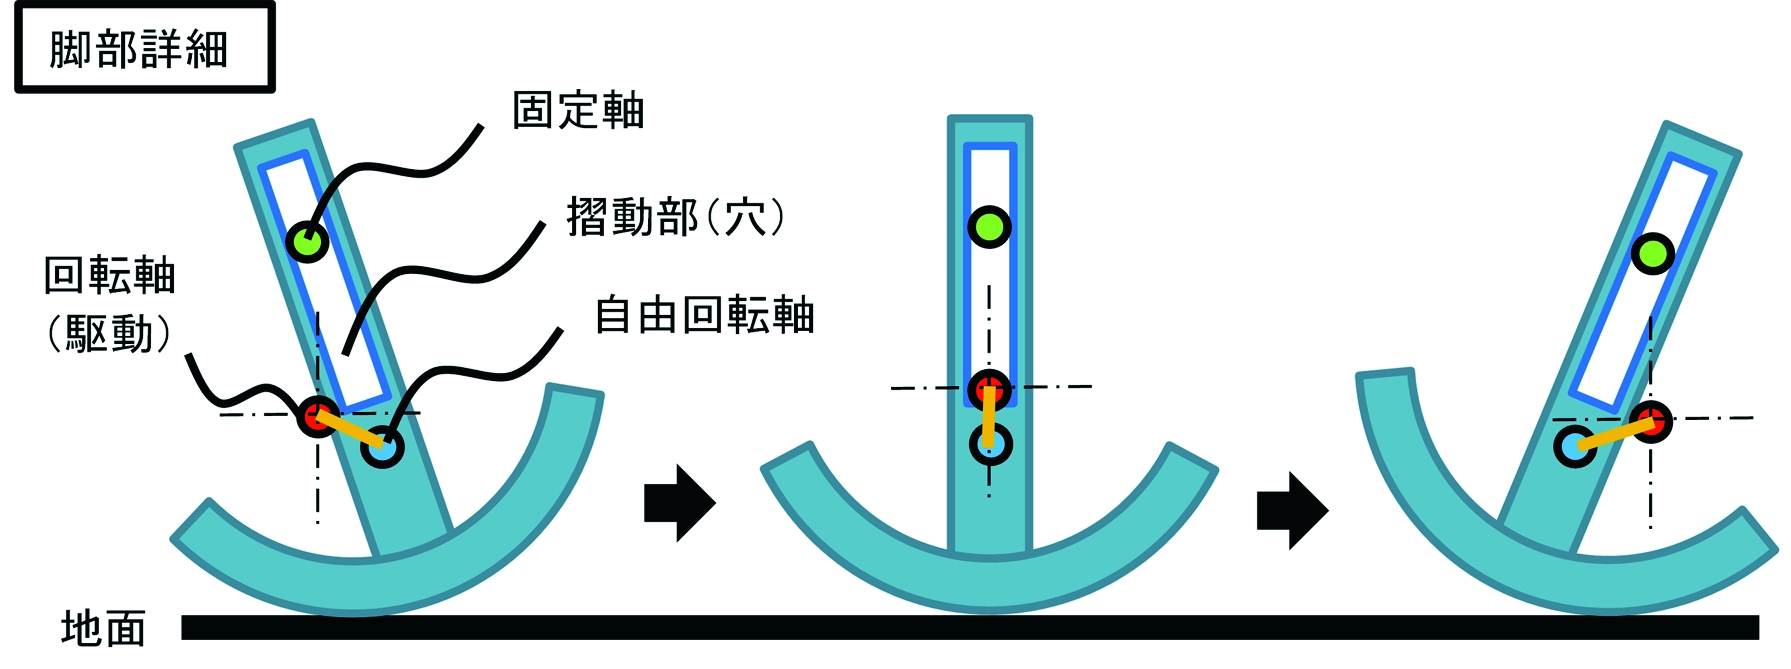
\includegraphics[width=300pt]{fig/fig02_cmyk.jpg}
\caption{脚構成 ポンチ絵}
\label{fig02}
\end{figure}

\subsection{アーム構成}\label{ux30a2ux30fcux30e0ux69cbux6210}

\begin{itemize}
\tightlist
\item
  リンク機構:スライダリンク機構を利用する。シンプルな構成であるため、強度の弱い材料で作っても問題が出にくいと考えた。
\item
  厚み:アームは相手機体と当接する部分なので、なるべく厚くし強度アップを狙う。
\item
  見た目:アームは機体の中でも最も目立つ部分。詳細設計時にはデザインにこだわる。
\end{itemize}

\begin{figure}[htbp]
\centering
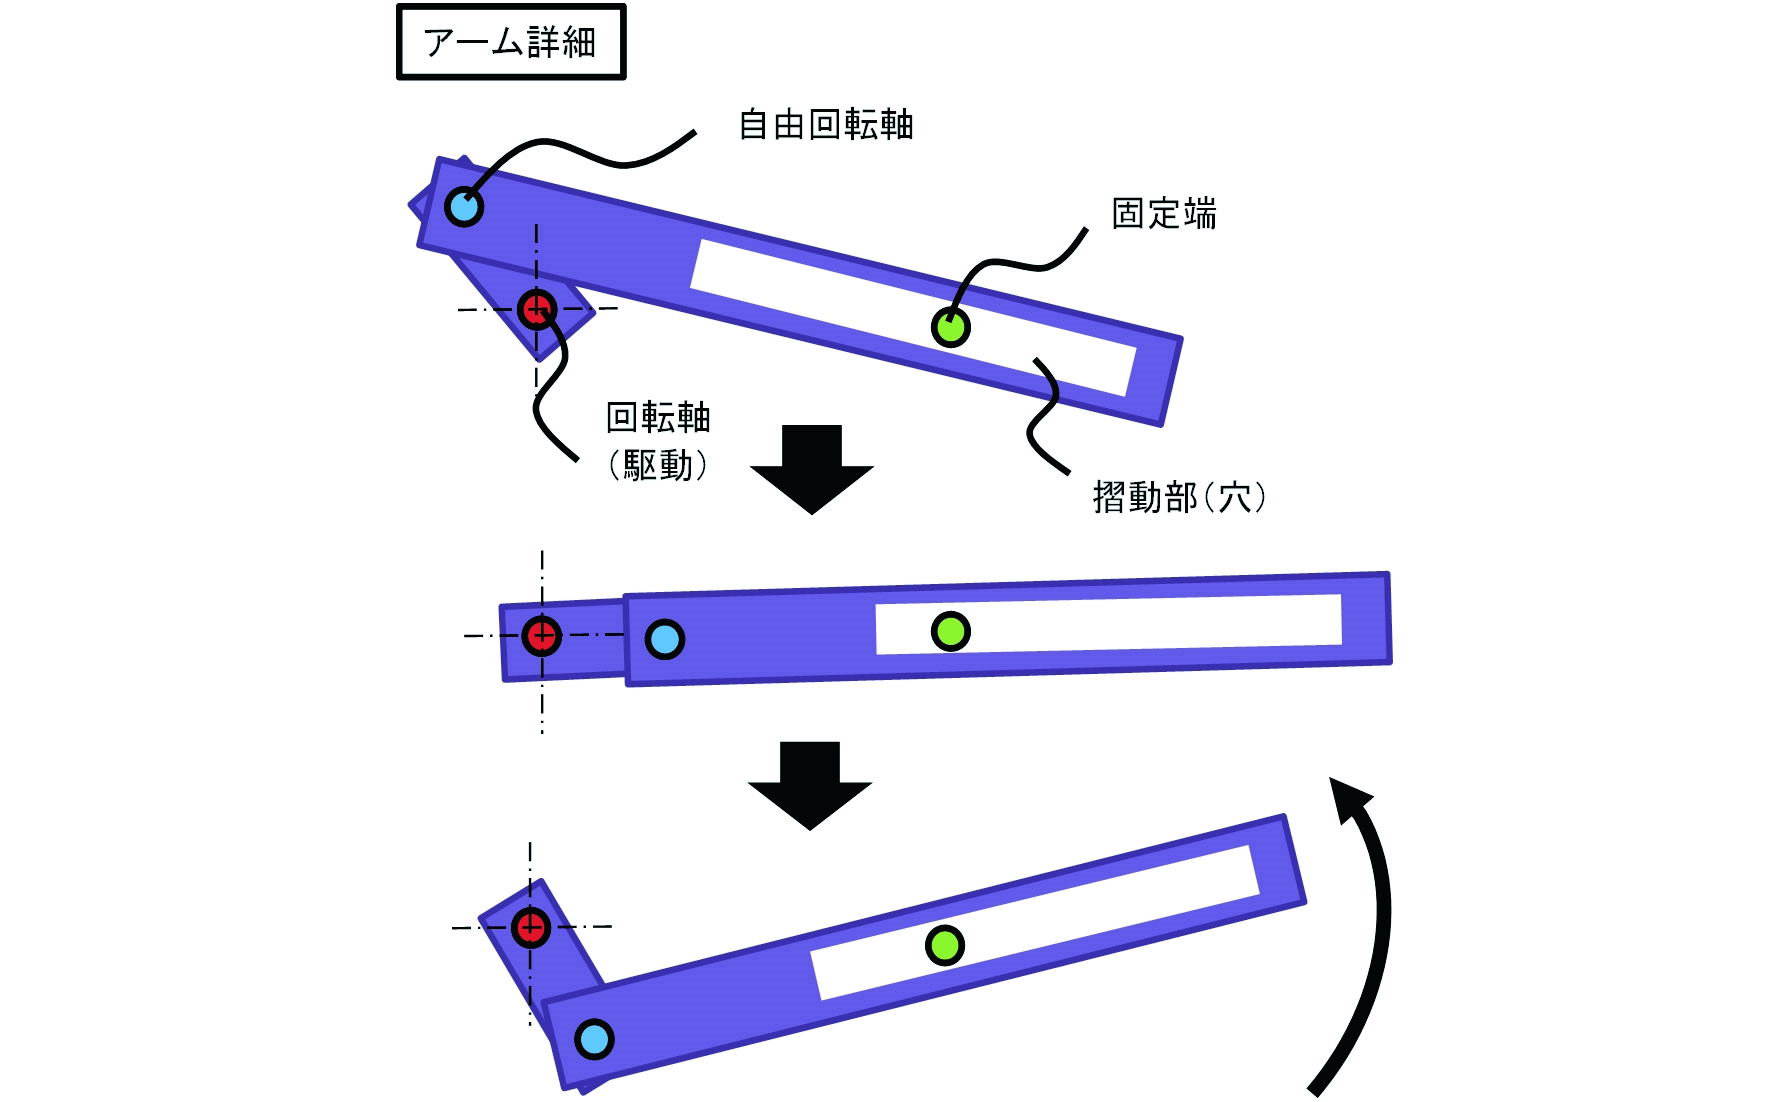
\includegraphics[width=380pt]{fig/fig03_cmyk.jpg}
\caption{アーム構成 ポンチ絵}
\label{fig03}
\end{figure}

\subsection{レイアウト設計}\label{ux30ecux30a4ux30a2ux30a6ux30c8ux8a2dux8a08}

構想設計が終わった後、レイアウト設計に移ります。
構成設計ではサイズ感が分からないため、規定サイズを念頭に置きながら大まかな機体サイズを決めていきます。
流れは下記の通りです。

\begin{itemize}
\tightlist
\item
  大会の規格サイズを確認:規定(2014年度)では機体サイズは幅250mm×奥行350mm×高さ700mm以内(停止時)
\item
  ポンチ絵をブロックで作成:感覚でユニットのサイズを決めてブロックを作成。細かい部品は作成しません。
\item
  ブロックを配置:規格サイズに合わせて、ユニットブロックをレイアウト
\end{itemize}

私が行った実例をFig.\ref{fig04}に示します。
ここまでいくと、脚部で使用できるスペースや、アームのサイズ感など、大まかに把握することができます。

使用したツールはCreo
Elements\cite{creo_elements}です。個人利用の範囲内なら無料で使用できます。

\begin{figure}[htbp]
\centering
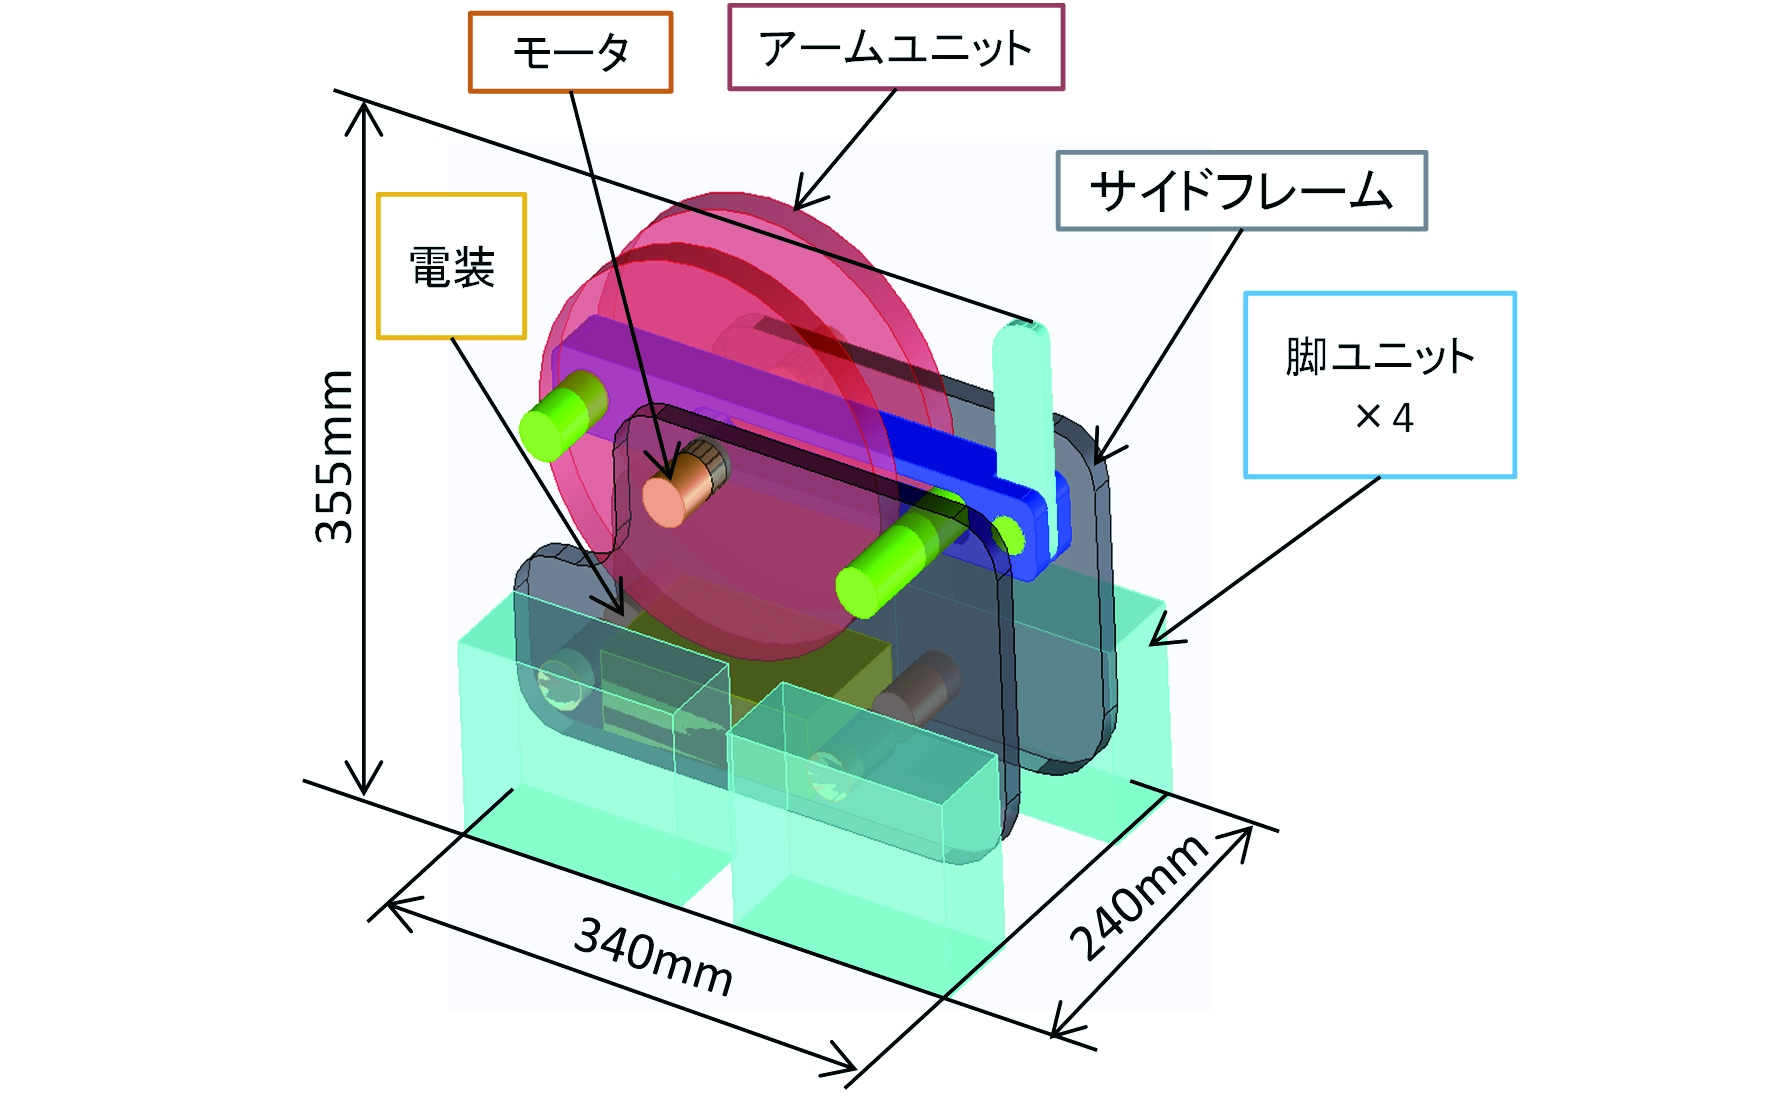
\includegraphics[width=380pt]{fig/fig04_cmyk.jpg}
\caption{レイアウト設計}
\label{fig04}
\end{figure}

\section{基本設計}\label{ux57faux672cux8a2dux8a08}

基本設計では構想設計を具体化するため、まずアクションアイテムを書き出しました。
3Dプリンタをフル活用するつもりでしたので、最も力が加わるアーム設計をケアした内容になっています。

\begin{enumerate}
\def\labelenumi{\arabic{enumi}.}
\tightlist
\item
  アーム設計パラメータ:大会規定と目標値から、各種設計パラメータを設定する
\item
  アーム強度計算:3Dプリンタによる部品で相手機体を持ち上げた時、破損しないように強度計算を行い、部品厚みを決定する
\item
  積層方向の割れ防止構成:3Dプリンタ積層方向に高負荷がかかると割れが発生しやすい。積層方向に力がかかる部品に関しては強度アップ構成を考える。
\item
  モータ出力部の削れ防止構成:モータ出力部と締結する3Dプリンタ部品が削れ、駆動伝達できなくなるリスクがある。信頼性の高い締結構成を考える。
\item
  大型部品の分割構成:3Dプリンタで作成できる部品サイズは、プリンタのテーブルサイズで決まる。大型部品の分割方法と締結方法を考える。
\end{enumerate}

\subsection{アーム設計パラメータ}\label{ux30a2ux30fcux30e0ux8a2dux8a08ux30d1ux30e9ux30e1ux30fcux30bf}

アーム設計パラメータとして、リンク機構の位置、クランク長さ、モータ個数、減速比があります。
対戦相手との間合いや持ち上げ高さ、等から決めるので、まずは目標値を定めました。

\begin{itemize}
\tightlist
\item
  アームの射程距離:作用点位置を機体前面から250mmとする
\item
  相手機体持ち上げ高さ:大会規格の200mm地点を通過する
\item
  相手機体持ち上げ力:3500g(機体重量の大会規格)を持ち上げる
\end{itemize}

\subsubsection{アーム設計パラメータ 計算モデル}\label{ux30a2ux30fcux30e0ux8a2dux8a08ux30d1ux30e9ux30e1ux30fcux30bfux8a08ux7b97ux30e2ux30c7ux30eb}

設計パラメータは相互に影響しあうため、独立して一つ一つを決定していくことが困難です。
例えば、アームの射程距離を短くすれば必要なモータ駆動力は少なくてよいが、アーム作用点の通過高さは低くなります。
一方で、アームの射程距離を長くすると必要なモータ駆動力も多く必要となり、アーム作用点の通過高さは高くなります。
そこで、各種パラメータを可視化&持ち上げ力計算ツールをExcelで作りました(Fig.\ref{fig05})。

\begin{itemize}
\tightlist
\item
  アームに駆動を与えるポイントを原点Oに設定
\item
  第1クランク部品の長さをL1とし、第2クランク部品の長さをL2と設定
\item
  第1クランク部品と第2クランク部品の接続ポイントを中間自由回転軸aに設定
\item
  第2クランク部品に設けた長穴と摺動するポイントを中間固定軸jに設定
\item
  作用点をcと設定し、作用力を計算から算出
\item
  駆動力の伝達力損失は無視
\end{itemize}

\begin{figure}[htbp]
\centering
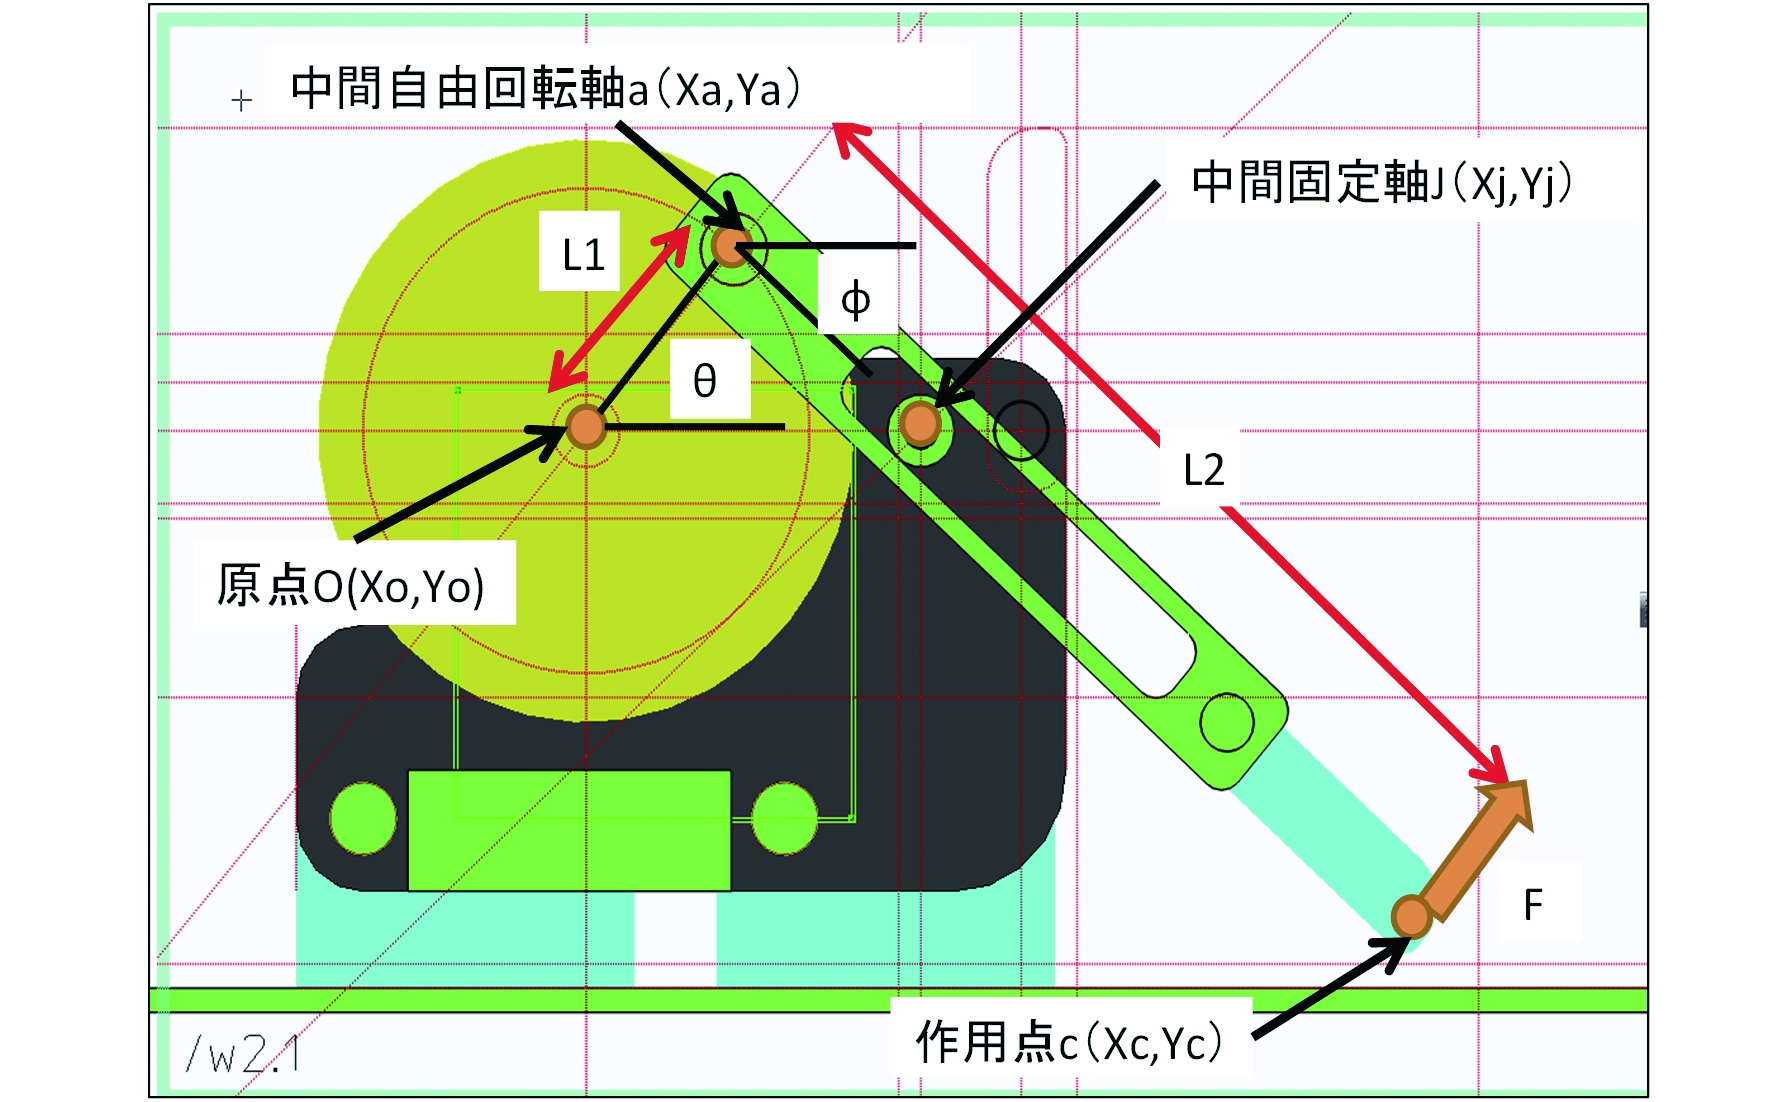
\includegraphics[width=270pt]{fig/fig05_cmyk.jpg}
\caption{アーム 計算モデル}
\label{fig05}
\end{figure}

\clearpage

\subsubsection{アーム設計パラメータ 計算結果とパラメータ決定}\label{ux30a2ux30fcux30e0ux8a2dux8a08ux30d1ux30e9ux30e1ux30fcux30bfux8a08ux7b97ux7d50ux679cux3068ux30d1ux30e9ux30e1ux30fcux30bfux6c7aux5b9a}

\begin{itemize}
\tightlist
\item
  アームの射程距離:作用点位置は機体前面から250mm
\item
  相手機体持ち上げ高さ:大会規格の200mm地点を通過
\item
  相手機体持ち上げ力:作用点で4208gfの力が出る(3500gf以上)
\end{itemize}

\begin{figure}[htbp]
\centering
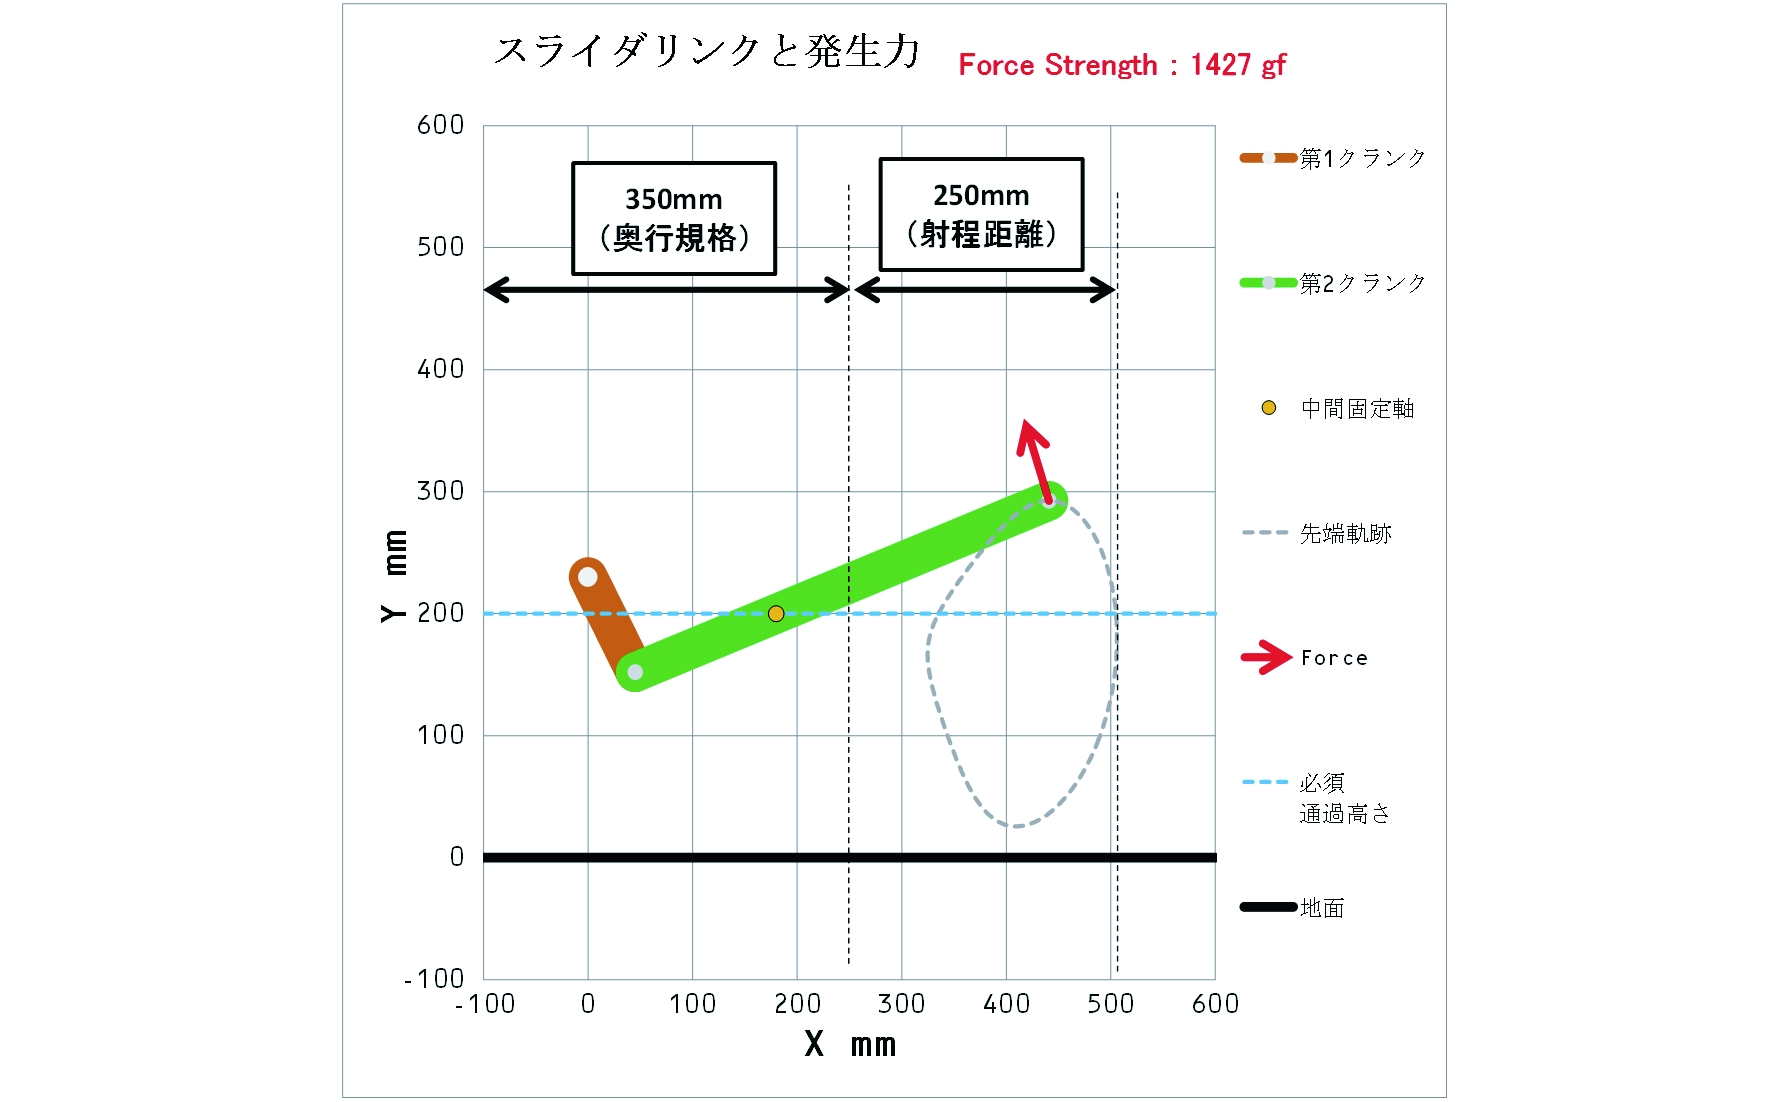
\includegraphics[width=390pt]{fig/fig07_cmyk.jpg}
\caption{アーム 計算結果}
\label{fig07}
\end{figure}

\begin{figure}[htbp]
\centering
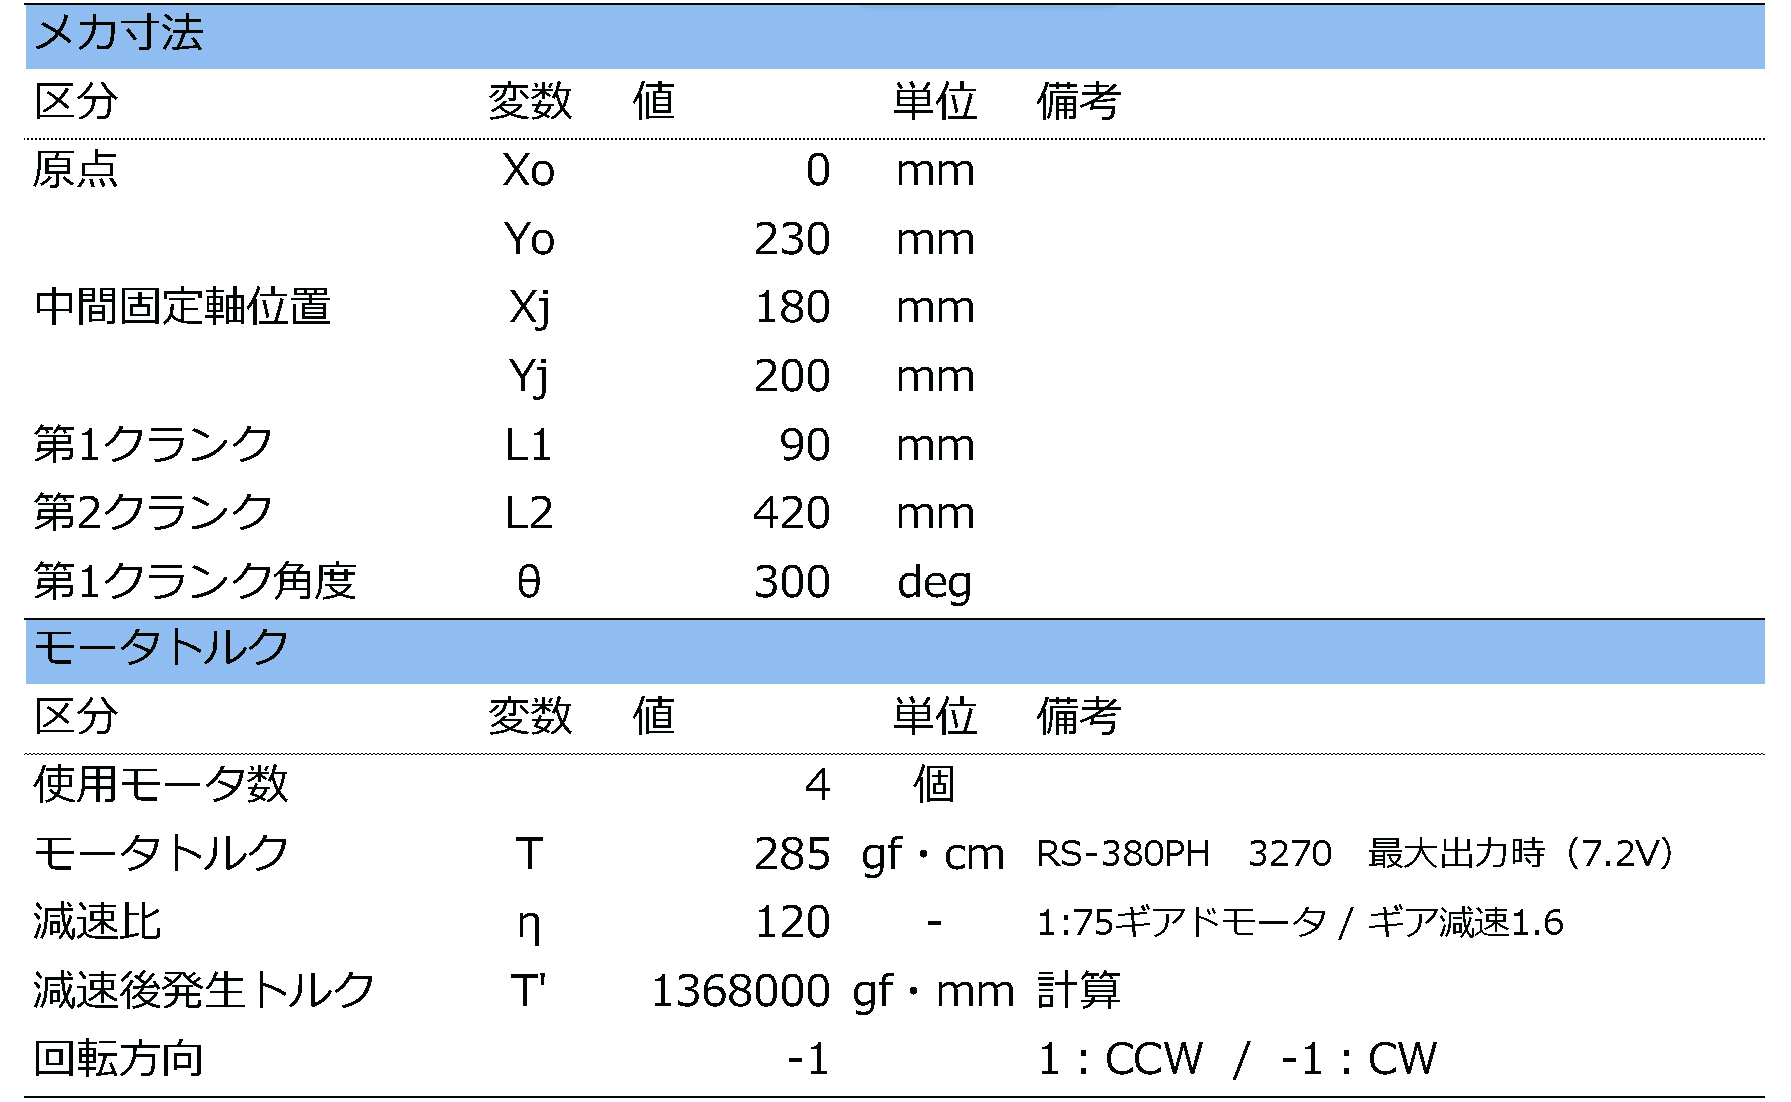
\includegraphics[width=250pt]{fig/fig06_cmyk.jpg}
\caption{アーム 設計パラメータの決定}
\label{fig06}
\end{figure}

\clearpage

\subsection{アーム強度計算}\label{ux30a2ux30fcux30e0ux5f37ux5ea6ux8a08ux7b97}

かわさきロボット競技大会では相手機体とぶつかるアーム部に最も強い力が加わるため、下記のような目標設定をしました

\begin{itemize}
\tightlist
\item
  作用点に3500g(機体重量の大会規格)が加わったときに破壊しないこと
\end{itemize}

計算モデルをFig.\ref{fig08}に示します。
部品名称はFig.\ref{fig05}と同様です。

\begin{itemize}
\tightlist
\item
  中間自由回転軸aを固定端と設定
\item
  作用点に3500gfが加わるように設定
\item
  アームの作用点に力が加わったときの第2クランク部品が中間固定軸から受ける力を計算
\item
  片持ち梁モデル計算からアームに加わる曲げ応力を計算
\item
  安全率は1.5、
  材料強度はABSの30\%と想定(3Dプリンタ樹脂充填率)して許容応力を計算
\end{itemize}

\begin{figure}[htbp]
\centering
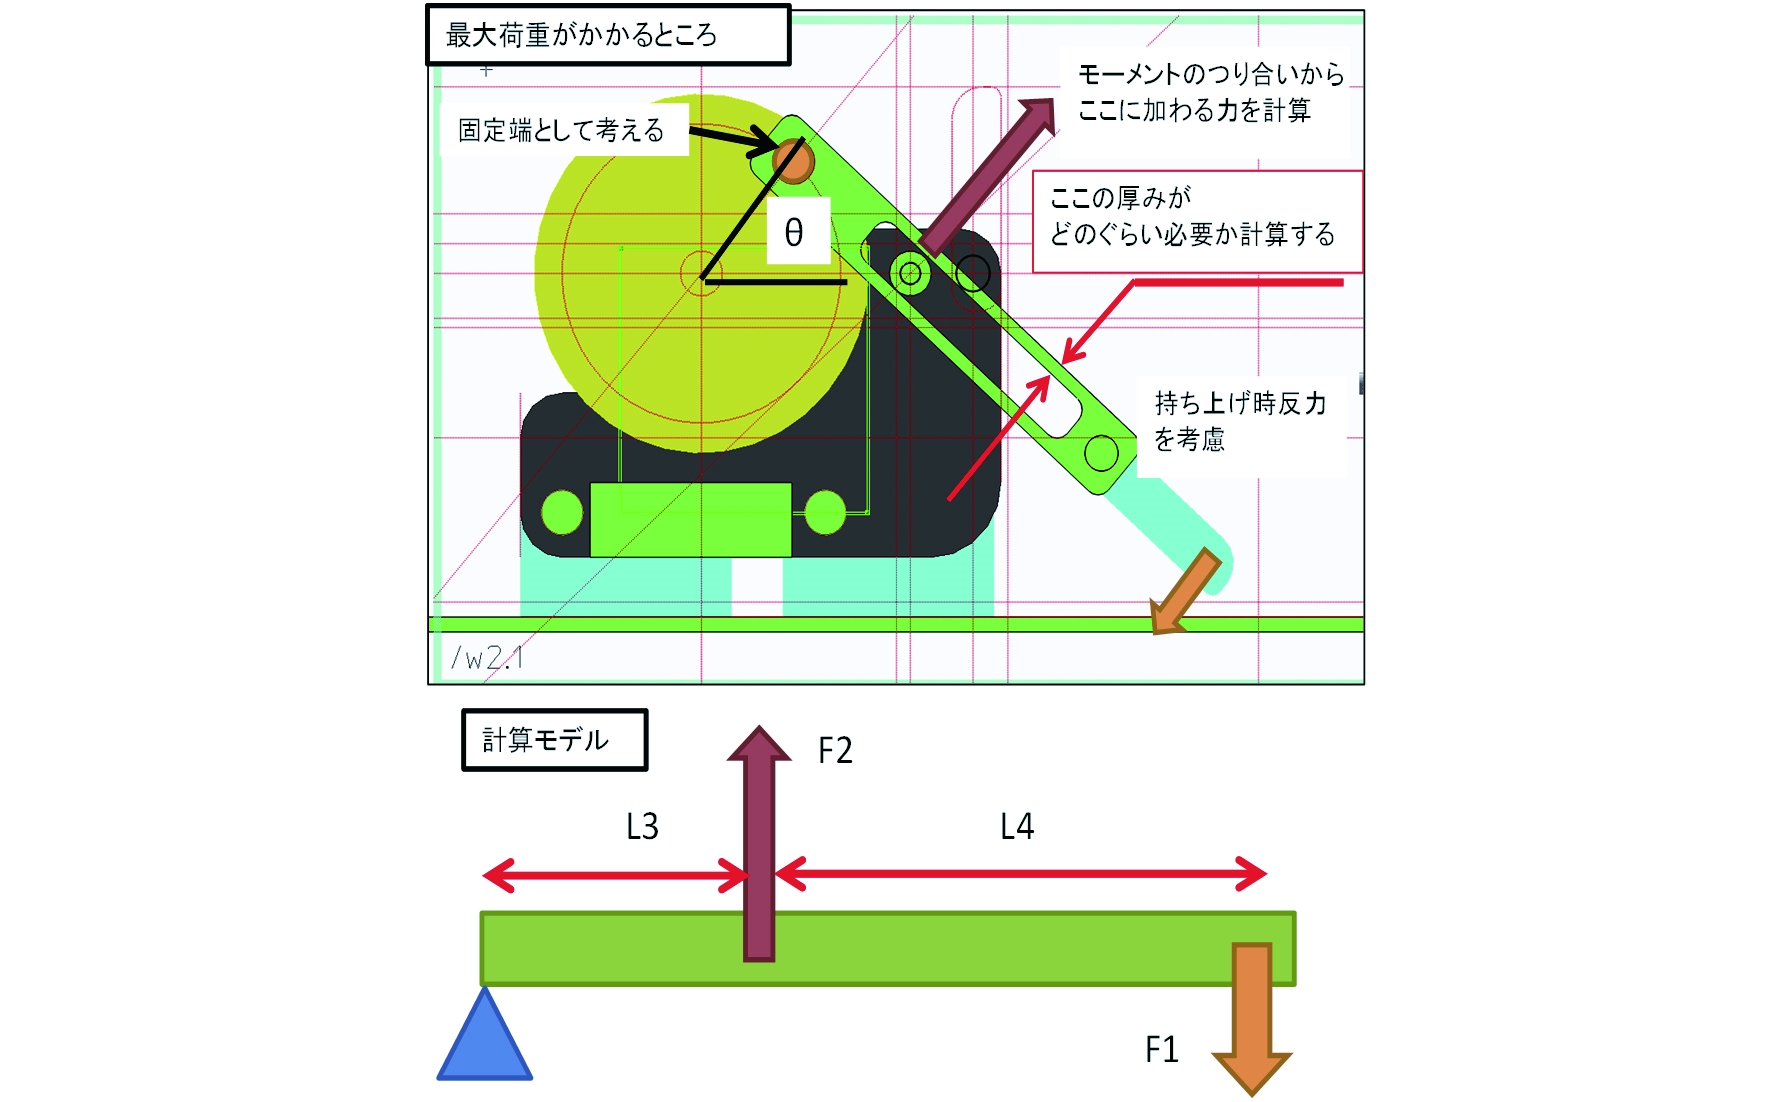
\includegraphics[width=450pt]{fig/fig08_cmyk.jpg}
\caption{強度計算 モデル}
\label{fig08}
\end{figure}

\clearpage

\subsubsection{計算結果とパラメータ設定}\label{ux8a08ux7b97ux7d50ux679cux3068ux30d1ux30e9ux30e1ux30fcux30bfux8a2dux5b9a}

\begin{itemize}
\tightlist
\item
  アームに加わる曲げ応力最大値:500gf/mm\textsuperscript{2}
  (許容曲げ応力:515gf/mm\textsuperscript{2} 以下)
\end{itemize}

\begin{figure}[htbp]
\centering
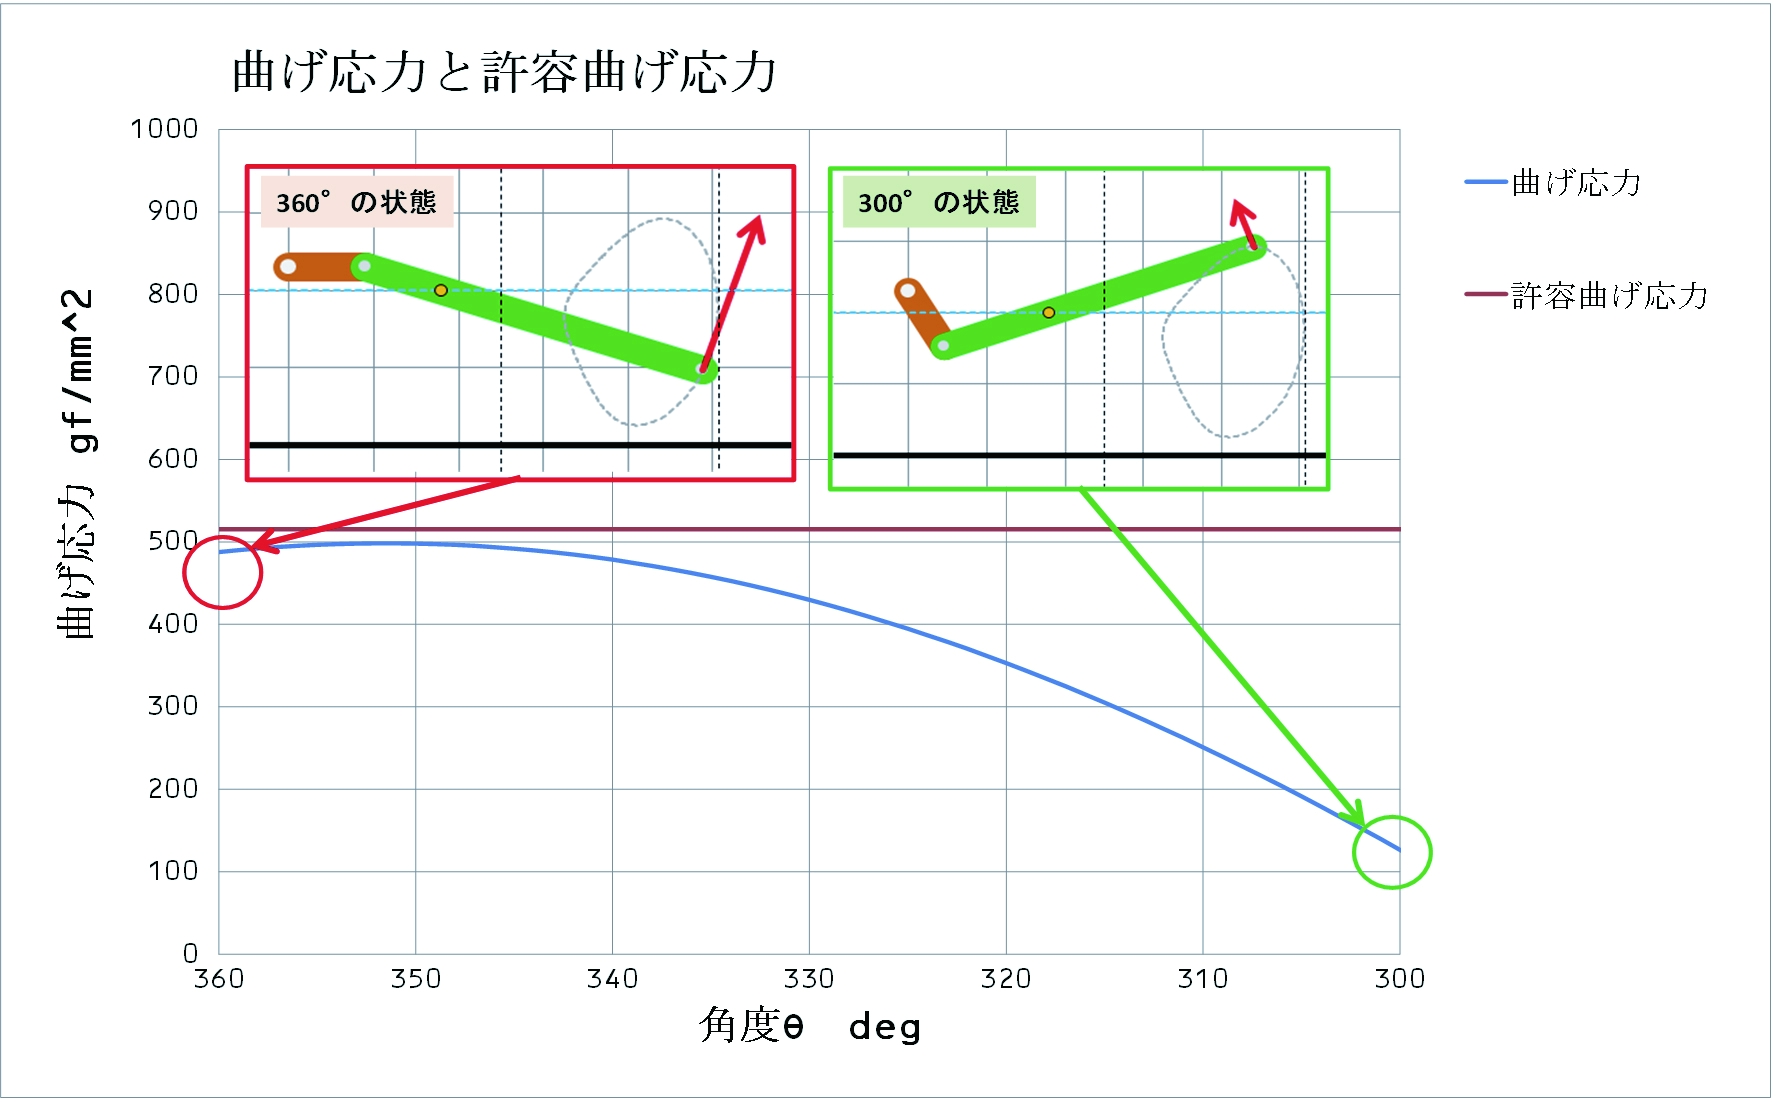
\includegraphics[width=380pt]{fig/fig09_cmyk.jpg}
\caption{強度計算 結果}
\label{fig09}
\end{figure}

上記結果となったときの設計パラメータはFig.\ref{fig10}の通りです。
部品幅を32mm以上、厚みを23mm以上とすればよい、という結果となりました。

\begin{figure}[htbp]
\centering
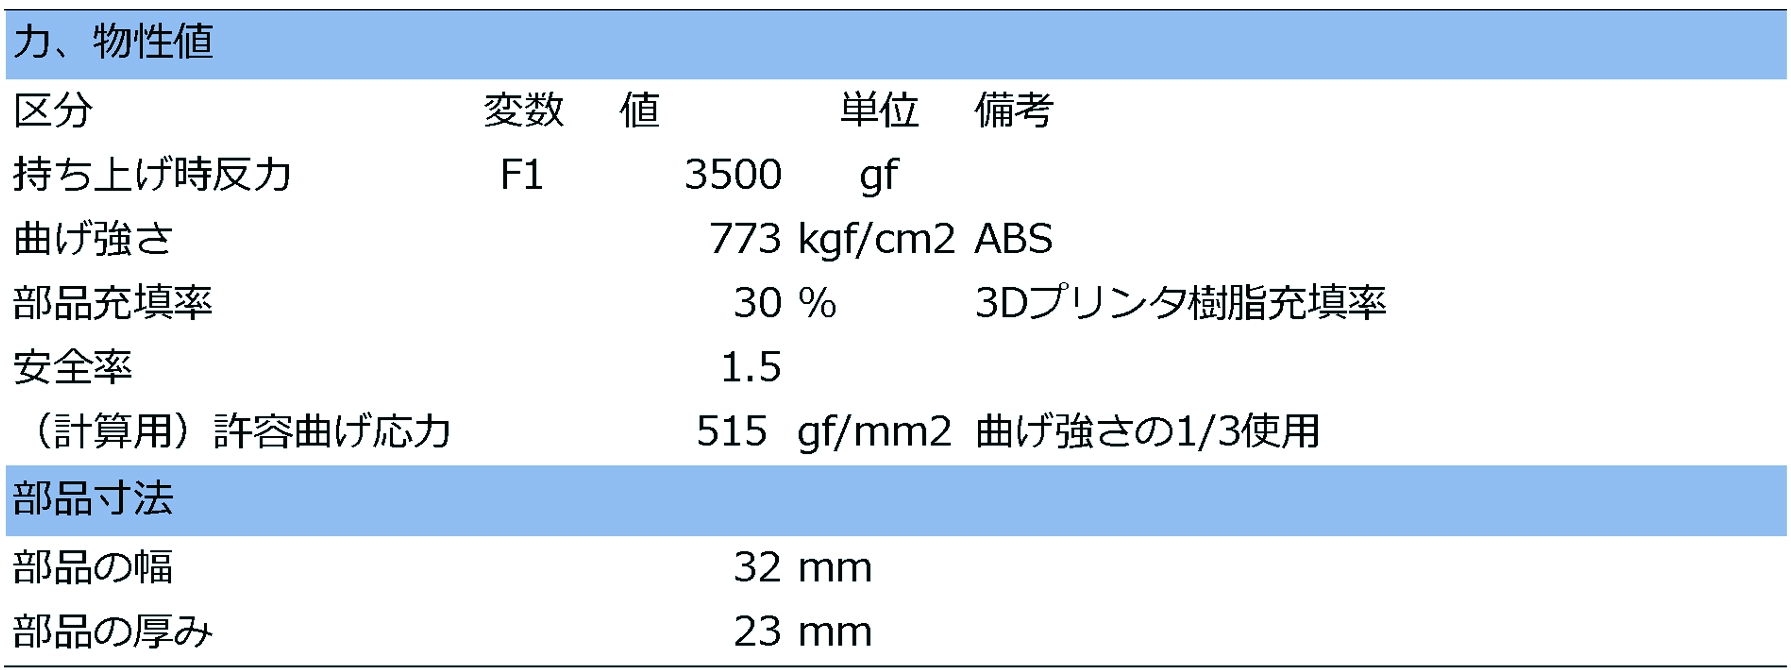
\includegraphics[width=350pt]{fig/fig10_cmyk.jpg}
\caption{強度設計 パラメータ}
\label{fig10}
\end{figure}

\clearpage

\subsection{積層方向の割れ防止構成}\label{ux7a4dux5c64ux65b9ux5411ux306eux5272ux308cux9632ux6b62ux69cbux6210}

第2章のおさらいになりますが、Fig.\ref{fig12}にFDM形式3Dプリンタの部品作成の様子を示します。
一層ずつ積層して形状を作り上げていくため、積層面が剥がれる方向の力に弱いです。

\begin{figure}[htbp]
\centering
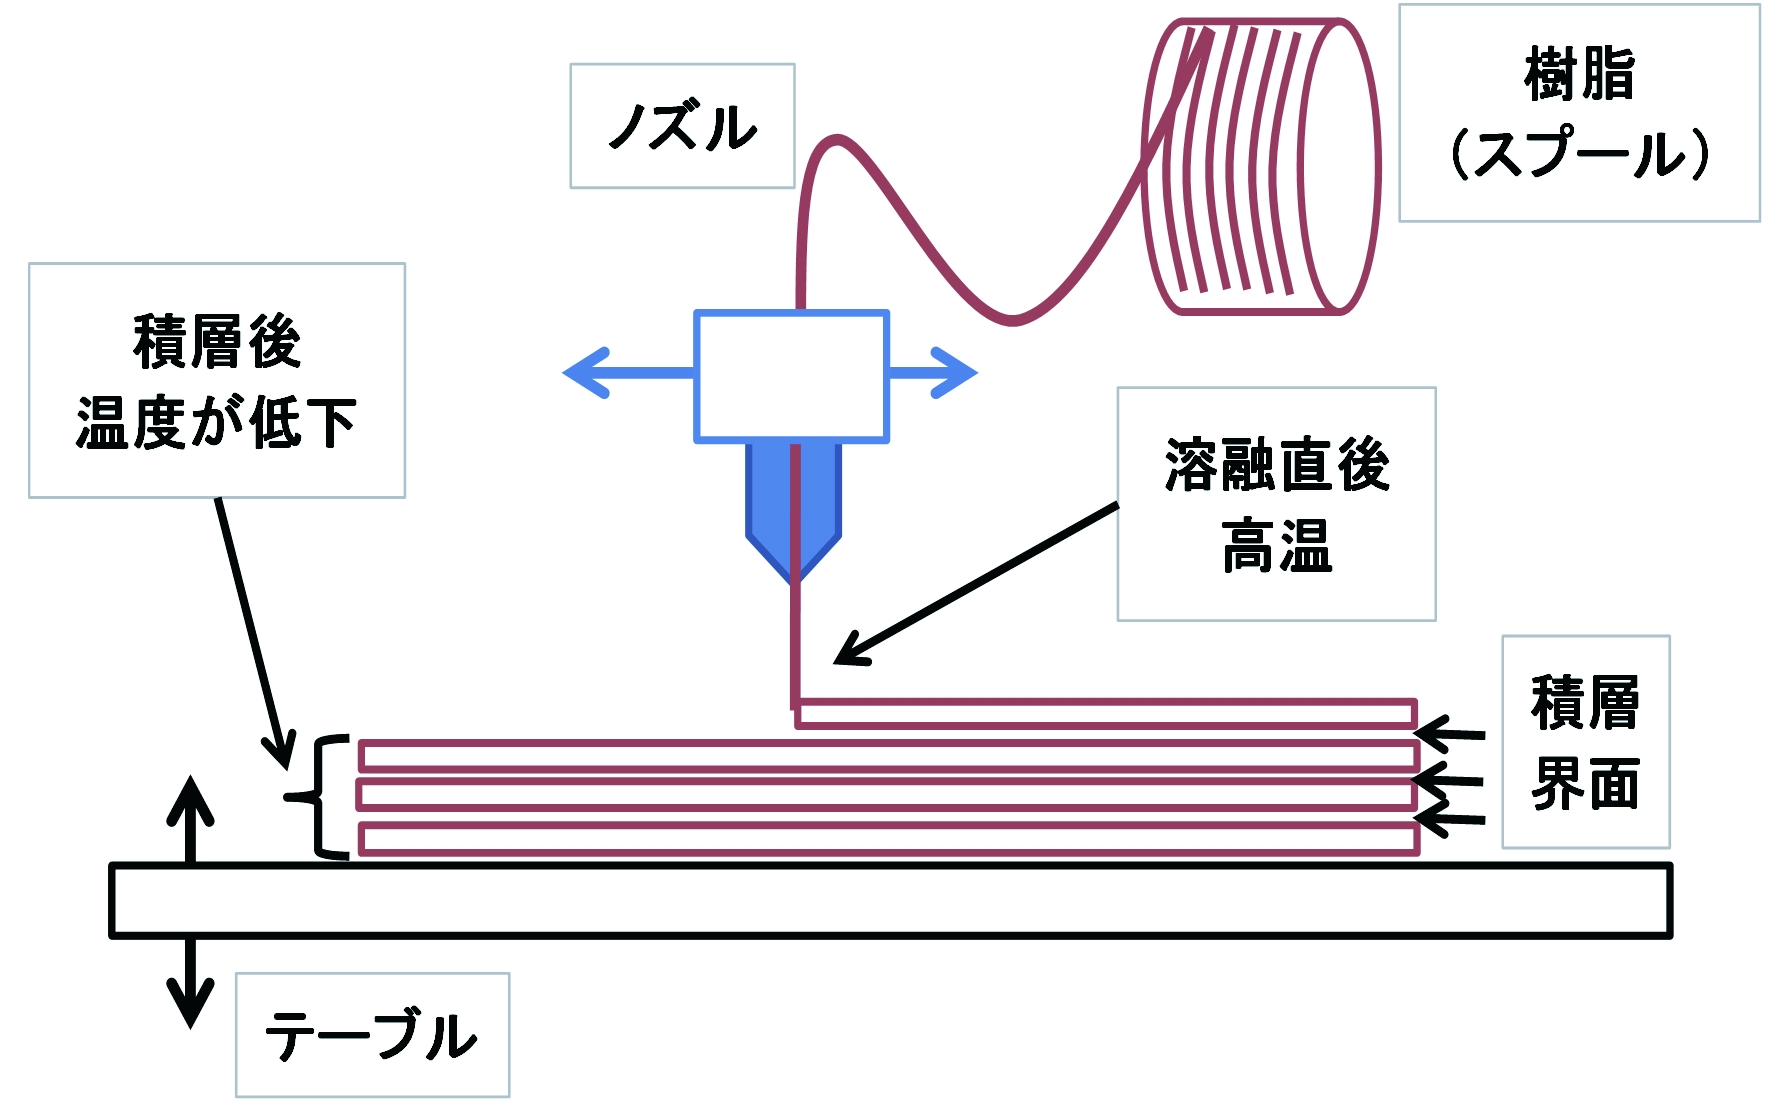
\includegraphics[width=250pt]{fig/fig12_cmyk.jpg}
\caption{3Dプリンタ(FDM方式) 部品作成の様子}
\label{fig12}
\end{figure}

\subsubsection{対策案}\label{ux5bfeux7b56ux6848}

上記のような積層方向に対する剥がれに対する強度は、樹脂温度や積層ピッチ等、様々な影響を受けるため机上計算は困難です。
 
そこで、積層方向に対して大きな力が加わる部品に関しては、できる限り破壊のリスクを減らすため図\ref{fig13}に示す構成を取ることとしました。
まず積層方向に対して力が加わる側の部品Aを中空形状とします。
次に積層方向を90°変更した補強部品Bを別途作成し、部品Aの中空部に圧入します。
この構成を取ることにより、積層方向に対して力が加わったとしても部品Bが力を受けてくれるため破壊しにくくなります。

\begin{figure}[htbp]
\centering
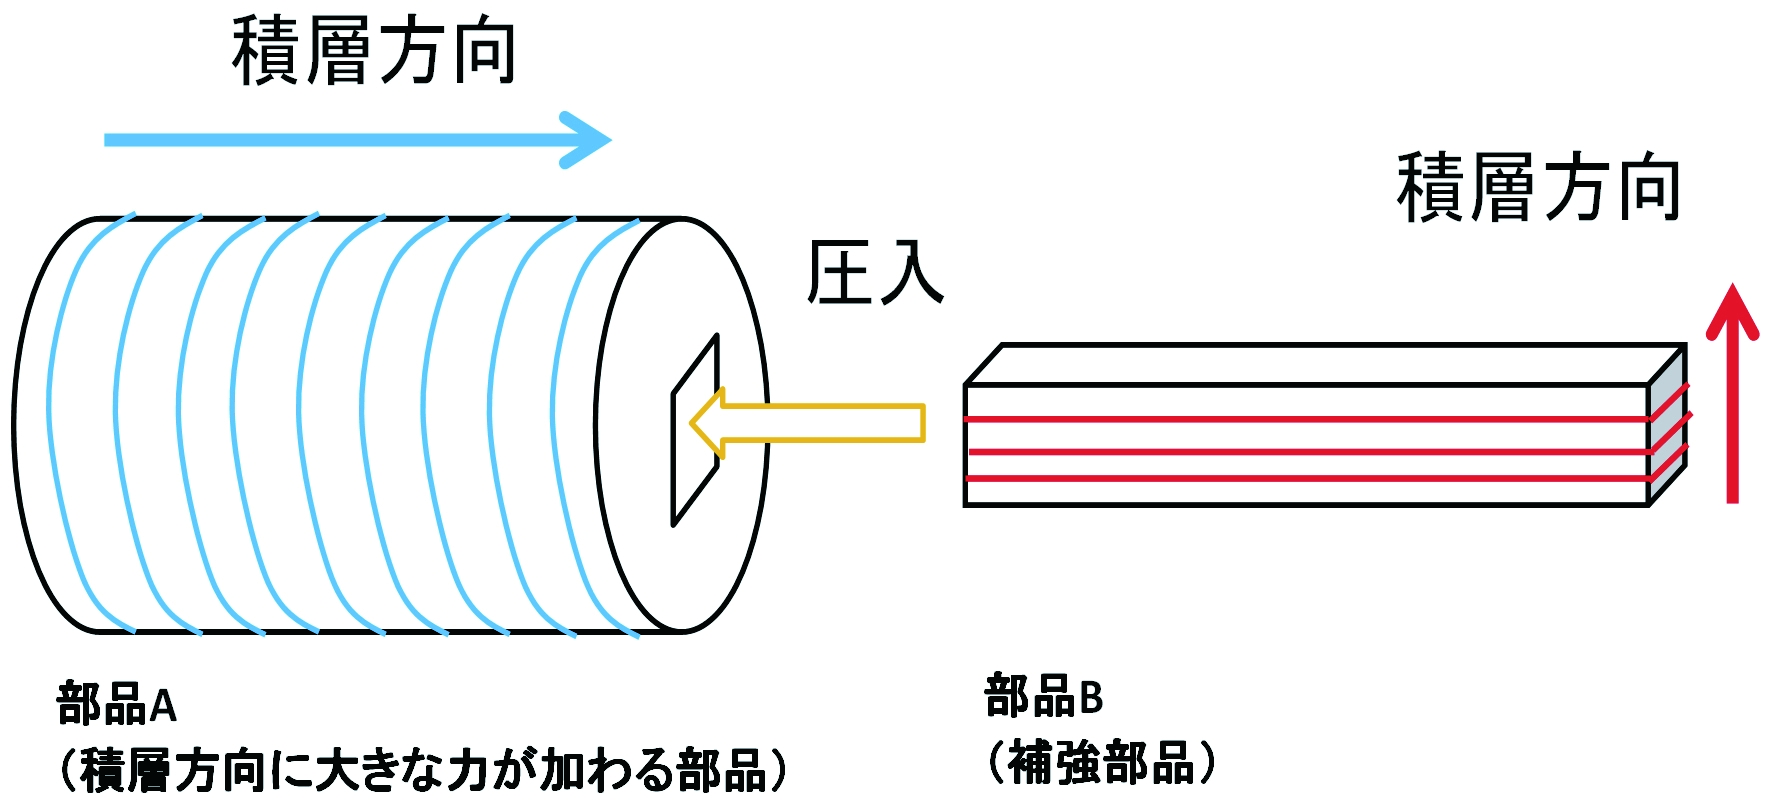
\includegraphics[width=250pt]{fig/fig13_cmyk.jpg}
\caption{積層方向 強度アップ構成}
\label{fig13}
\end{figure}

\clearpage

\subsection{モータ出力部の削れ防止構成}\label{ux30e2ux30fcux30bfux51faux529bux90e8ux306eux524aux308cux9632ux6b62ux69cbux6210}

駆動構成のシンプル化のため、本機体の脚部・アーム部の駆動モータにタミヤのギアドモータ380K\cite{tamiya_380k}を採用することにしました。
ギアドモータの出力部はDカットされた出力軸から駆動を伝達する必要があります。
ギアドモータの出力軸径はφ6mmと細いため、直接3Dプリンタで作成した部品へ駆動を伝達するとFig.\ref{fig14}のようにDカット部で削れが生じます。
削れが進行すると、最悪駆動伝達ができなくなる恐れがあります。

\begin{figure}[htbp]
\centering
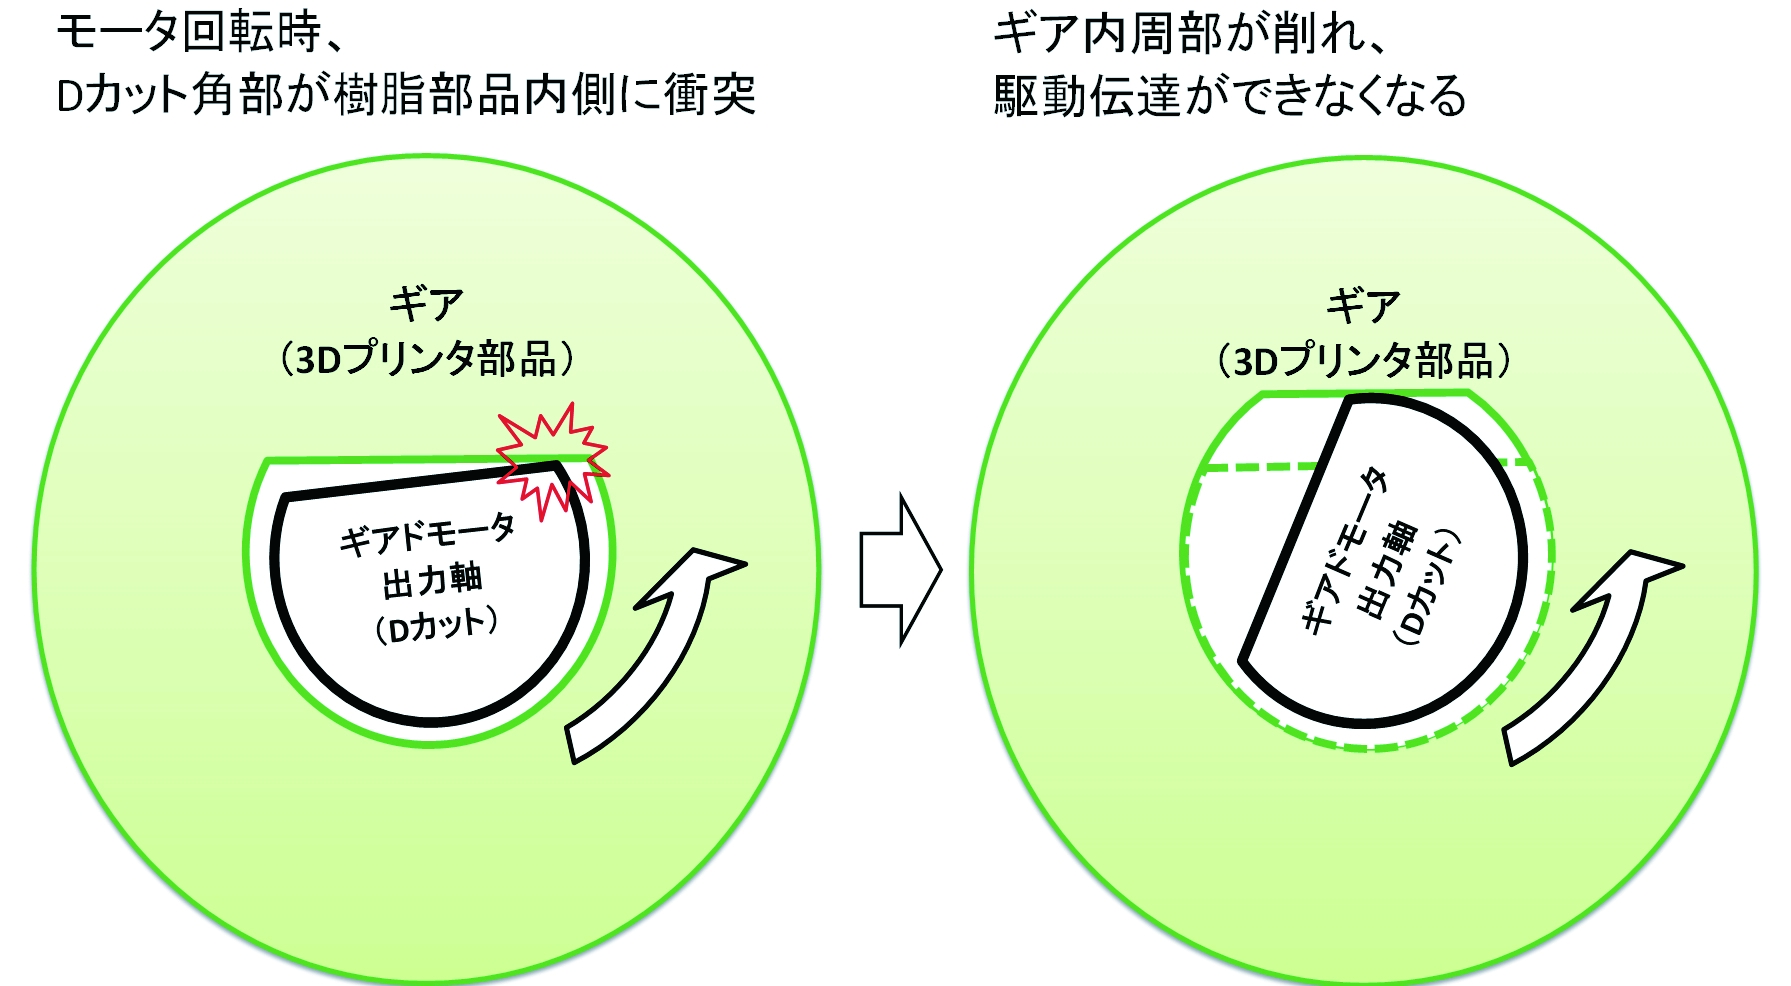
\includegraphics[width=280pt]{fig/fig14_cmyk.jpg}
\caption{ギア削れの様子}
\label{fig14}
\end{figure}

そこで、モータ出力を受け取る部分だけは、金属(今回はアルミ)で部品を作成することとしました。
この金属部品から3Dプリンタで作成した部品へ駆動を伝達することで、モータ出力部の削れを防止します。

\subsection{大型部品の作成方法}\label{ux5927ux578bux90e8ux54c1ux306eux4f5cux6210ux65b9ux6cd5}

3Dプリンタはテーブルサイズ以上のサイズの部品は作ることができません。
私の所有している3Dプリンター\cite{replicator2x}のテーブルサイズは246mm×152mm×155mmです。

一方、かわさきロボット競技大会のサイズ規格は幅250mm×奥行350mm×高さ700mmですので、
テーブルサイズ以上の部品を作るための構成を考えました。

\begin{itemize}
\tightlist
\item
  複数部品を嵌め合わせて大型部品を構成
\item
  強度確保のため厚みを十分に確保
\item
  はめ込み形状を利用して部品同士を結合させる
\item
  ねじれにも強いはめ込み形状
\end{itemize}

実施例詳細は、詳細設計で説明します。


\chapter{3Dプリンタでロボット製作}
\thispagestyle{fancy}
\section{全体構成}\label{ux5168ux4f53ux69cbux6210}

\subsection{概略}\label{ux6982ux7565}

機体の全体図をFig.\ref{fig15}に示します。

この機体は底部フレームを土台として、脚ユニットが4つ締結されています。
底部フレームは箱型形状をしており、内側にはバッテリーや制御回路などの電装系が内蔵されています。
この構成により、機体組立後は外側から電装系にアクセスできないようになっています。

中間フレームは底部フレームの天面に取り付けられ、蓋の役割も兼ねています。
中間フレームには2枚の側面フレームが締結され、左右のフレーム間にアームの全部品が取り付けられています。

脚部を駆動するギアドモータは各脚に1つずつ搭載されており、アームにも独立したモータが搭載されています。

次に機体の分解図をFig.\ref{fig16}に示します。

中間フレームは、底部フレームとネジ2本だけで締結されており、底部フレームと中間フレームは容易に組立・分解が可能です。
また、脚ユニットは4つ全て共通であるため、どの場所にでも取り付けることが可能です。

脚ユニットの取り付け方法ですが、底部フレームを挟み込んだ後に、ネジ1本のみで固定する構成としました。
故障時の交換対応がしやすくなっています。
これによりメンテナンス性の向上を狙っています。

\begin{figure}[htbp]
\centering
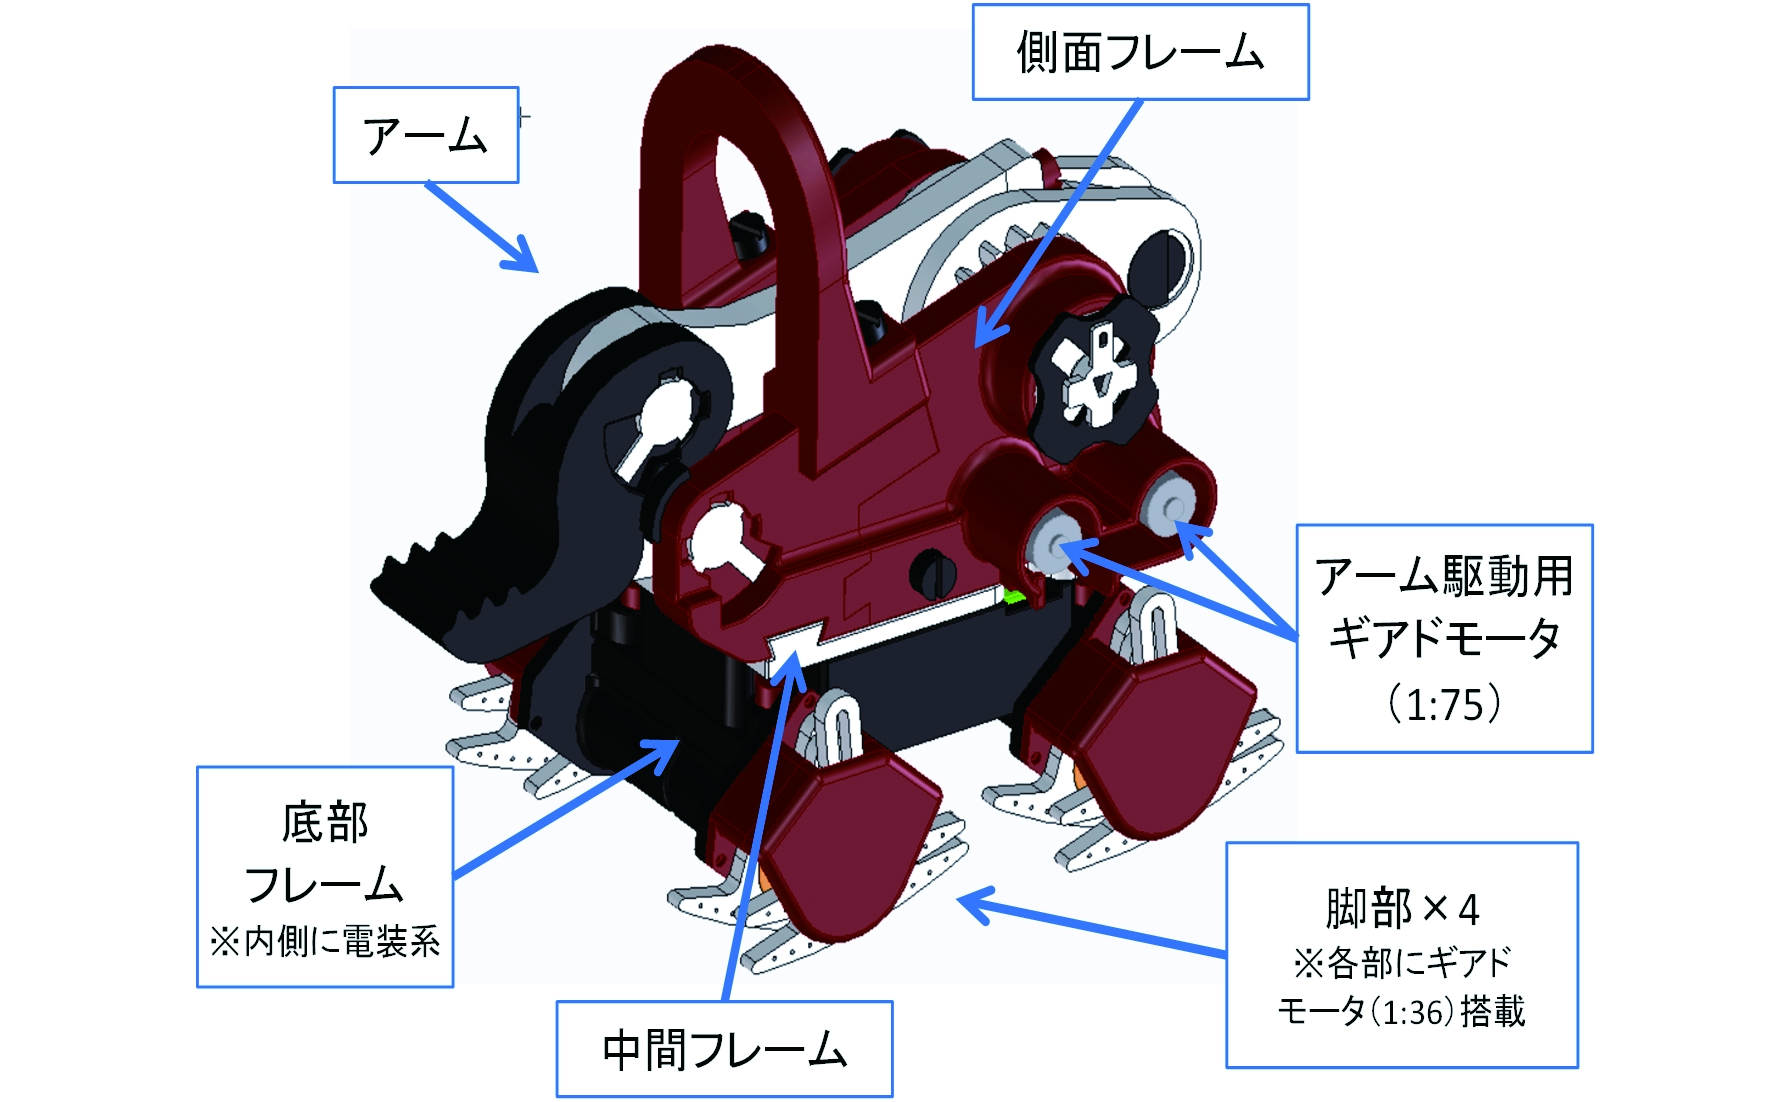
\includegraphics[width=400pt]{fig/fig15_cmyk.jpg}
\caption{機体の全体像}
\label{fig15}
\end{figure}

\begin{figure}[htbp]
\centering
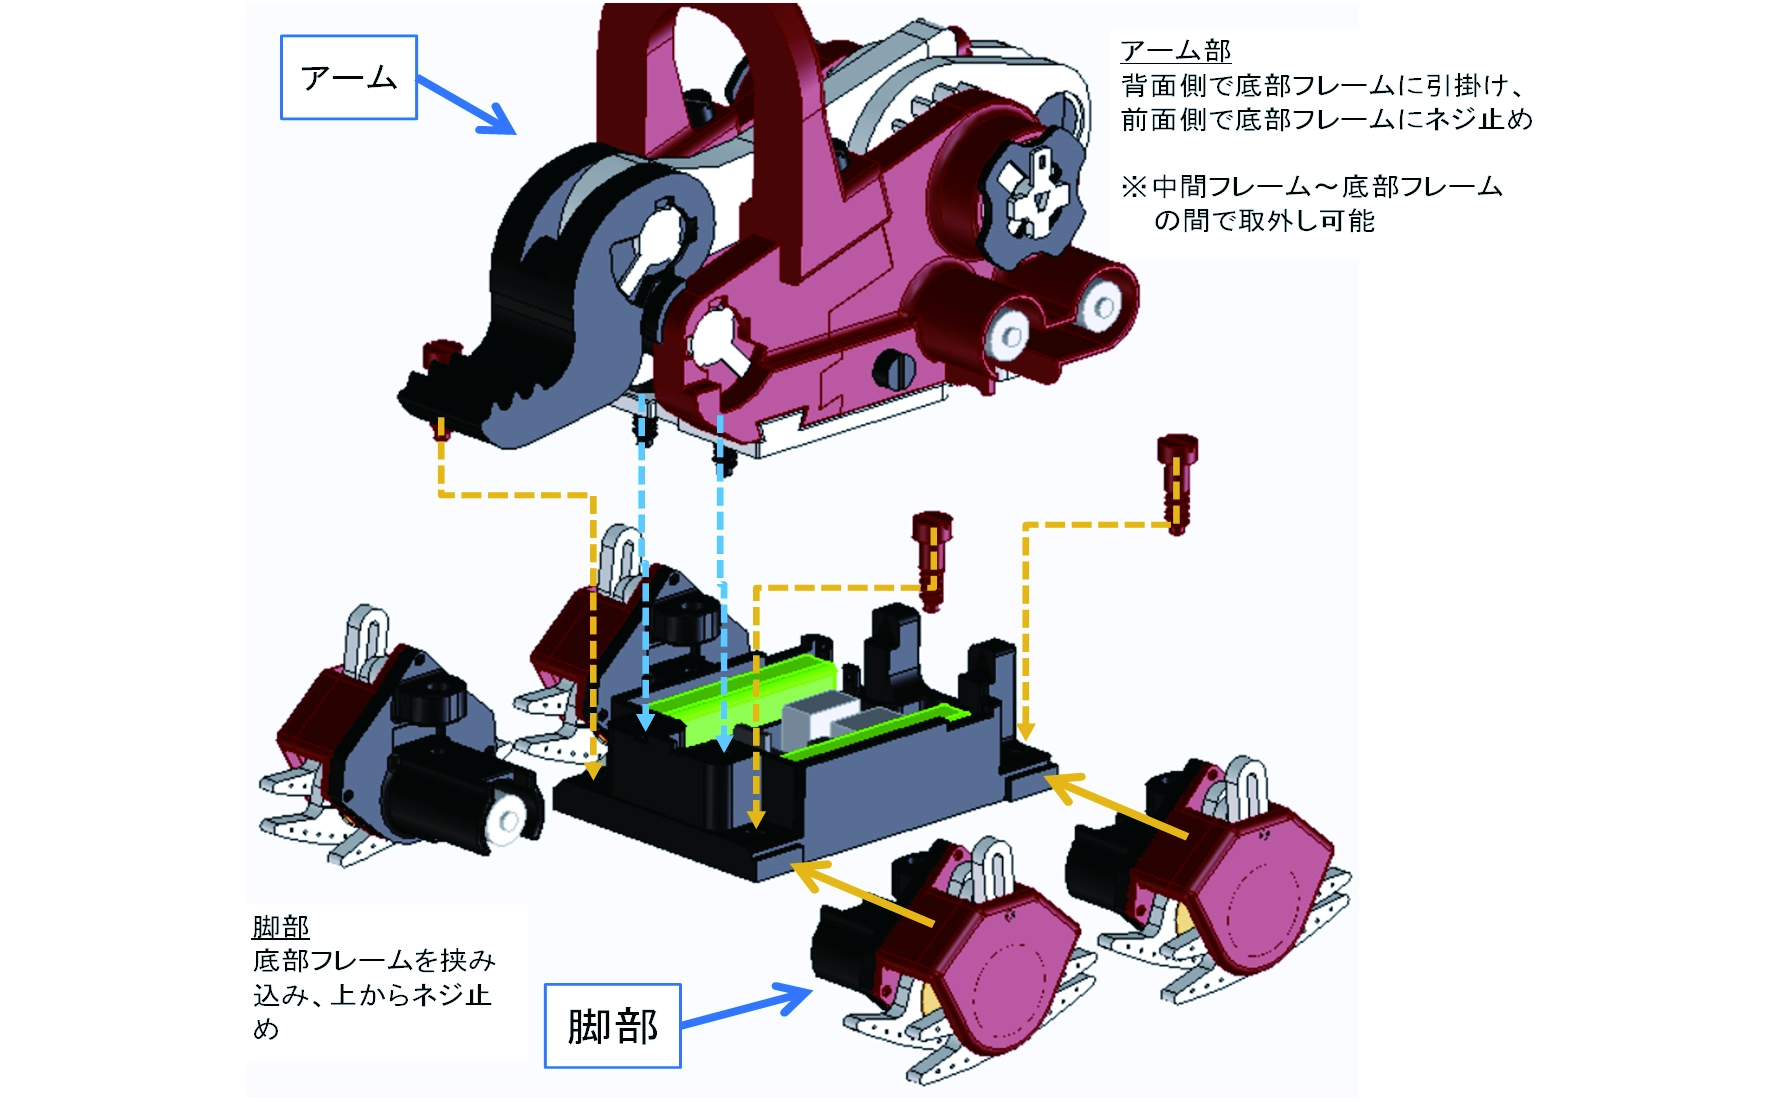
\includegraphics[width=400pt]{fig/fig16_cmyk.jpg}
\caption{機体の分解図}
\label{fig16}
\end{figure}

\clearpage

\subsection{機体の状態とサイズ}\label{ux6a5fux4f53ux306eux72b6ux614bux3068ux30b5ux30a4ux30ba}

機体の各状態とサイズの関係は下記の通りに設計しました。

\begin{itemize}
\tightlist
\item
  Fig.\ref{fig17}(a)
  停止状態。規格サイズに収まるようにアーム先端を分割し、アーム長を短くした状態で待機しています
\item
  Fig.\ref{fig17}(b)
  走行時の状態。開始直後にアームを動かすと、アーム先端が自重で回転しアーム長が伸びます
\item
  Fig.\ref{fig17}(c)
  相手機体攻撃時の状態を示した斜視図。基本設計で検討した通り射程距離は機体全面から250mmとなっています
\end{itemize}

\begin{figure}[htbp]
\centering
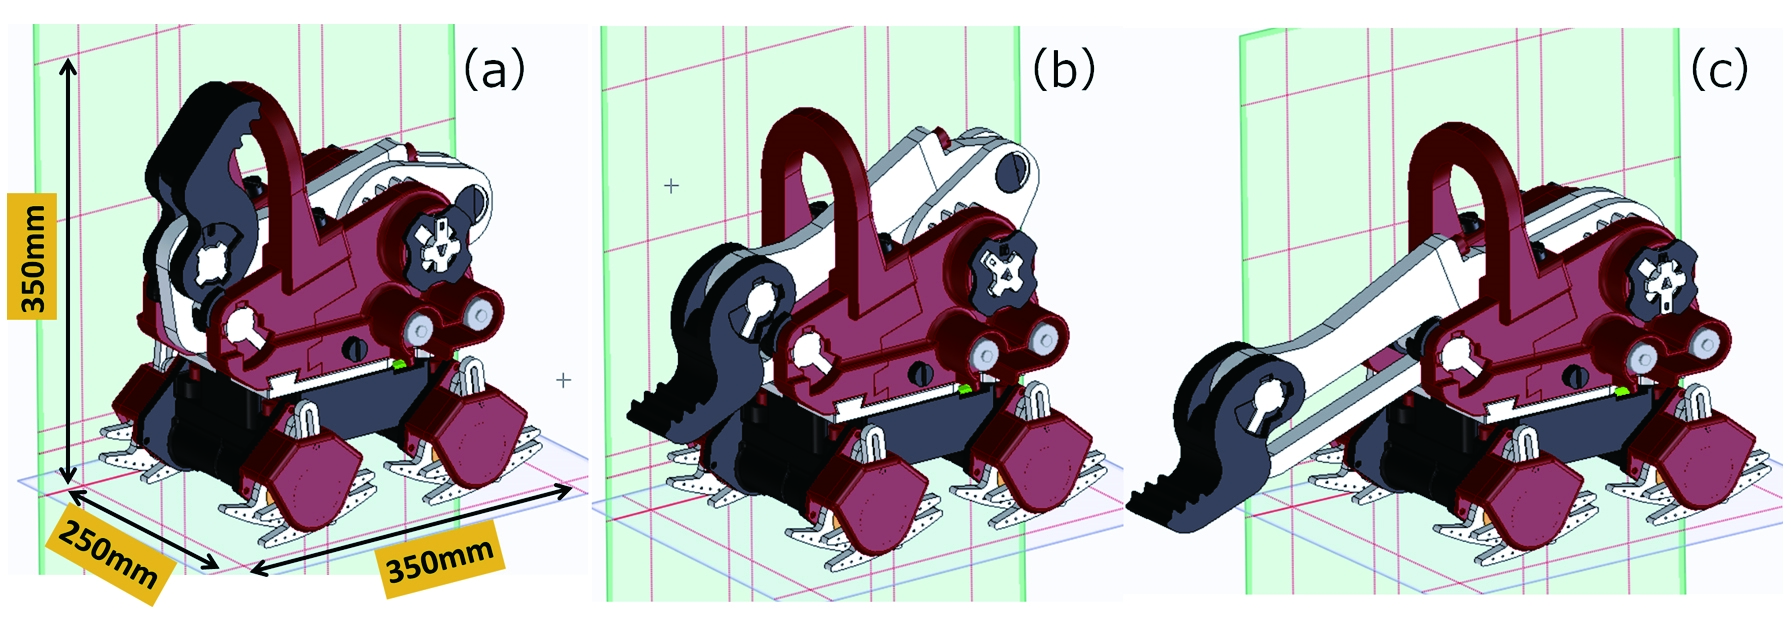
\includegraphics[width=380pt]{fig/fig17_cmyk.jpg}
\caption{機体の状態とサイズ}
\label{fig17}
\end{figure}

\section{アーム構成の詳細}\label{ux30a2ux30fcux30e0ux69cbux6210ux306eux8a73ux7d30}

アーム構成は第3章で決定したパラメータで設計を行った。
側面からみた断面図を Fig.\ref{fig18}に示します。

アーム駆動用ギアドモータ(1:75)は小ギアに接続されており、合計4つのギアドモータの駆動力がアームへと伝達されます。
駆動伝達経路は、ギアドモータ、小ギア、大ギア(第1クランクと接合されている)となっています。
小ギアと大ギアの減速比は第3章で計算した通り、1.6としています。

アームの第2クランクには相手機体攻撃時に大きな力が加わります。
こちらも第3章で計算した通り、幅32mm以上、厚み23mm以上を確保して設計しています。

実際に必要強度が確保されているかは不明ですが、試合時にアーム部の部品破損は発生しませんでした。
実用上は問題ないレベルで設計できていたのではないかと思います。

\begin{figure}[htbp]
\centering
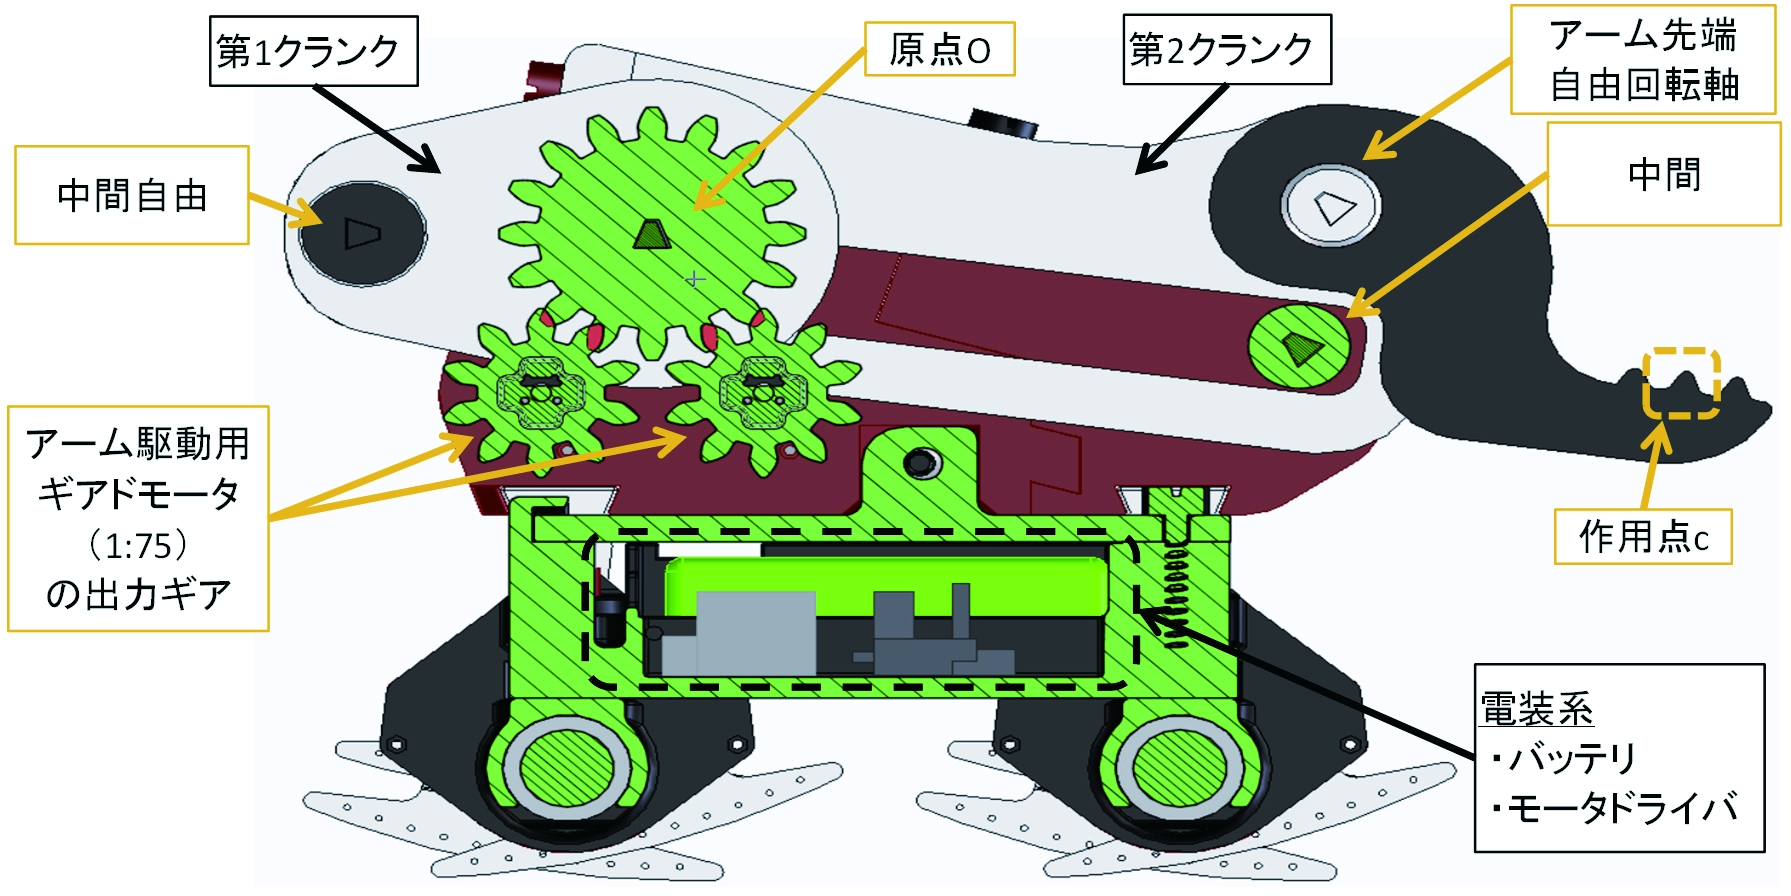
\includegraphics[width=380pt]{fig/fig18_cmyk.jpg}
\caption{アーム構成}
\label{fig18}
\end{figure}

\section{積層方向の割れ防止構成}\label{ux7a4dux5c64ux65b9ux5411ux306eux5272ux308cux9632ux6b62ux69cbux6210}

負荷がかかる部分に関しては積層方向の割れ防止構成を盛り込んで設計を行いました。
負荷のかかる箇所と実際の設計構成をFig.\ref{fig20}に示します。

\begin{figure}[htbp]
\centering
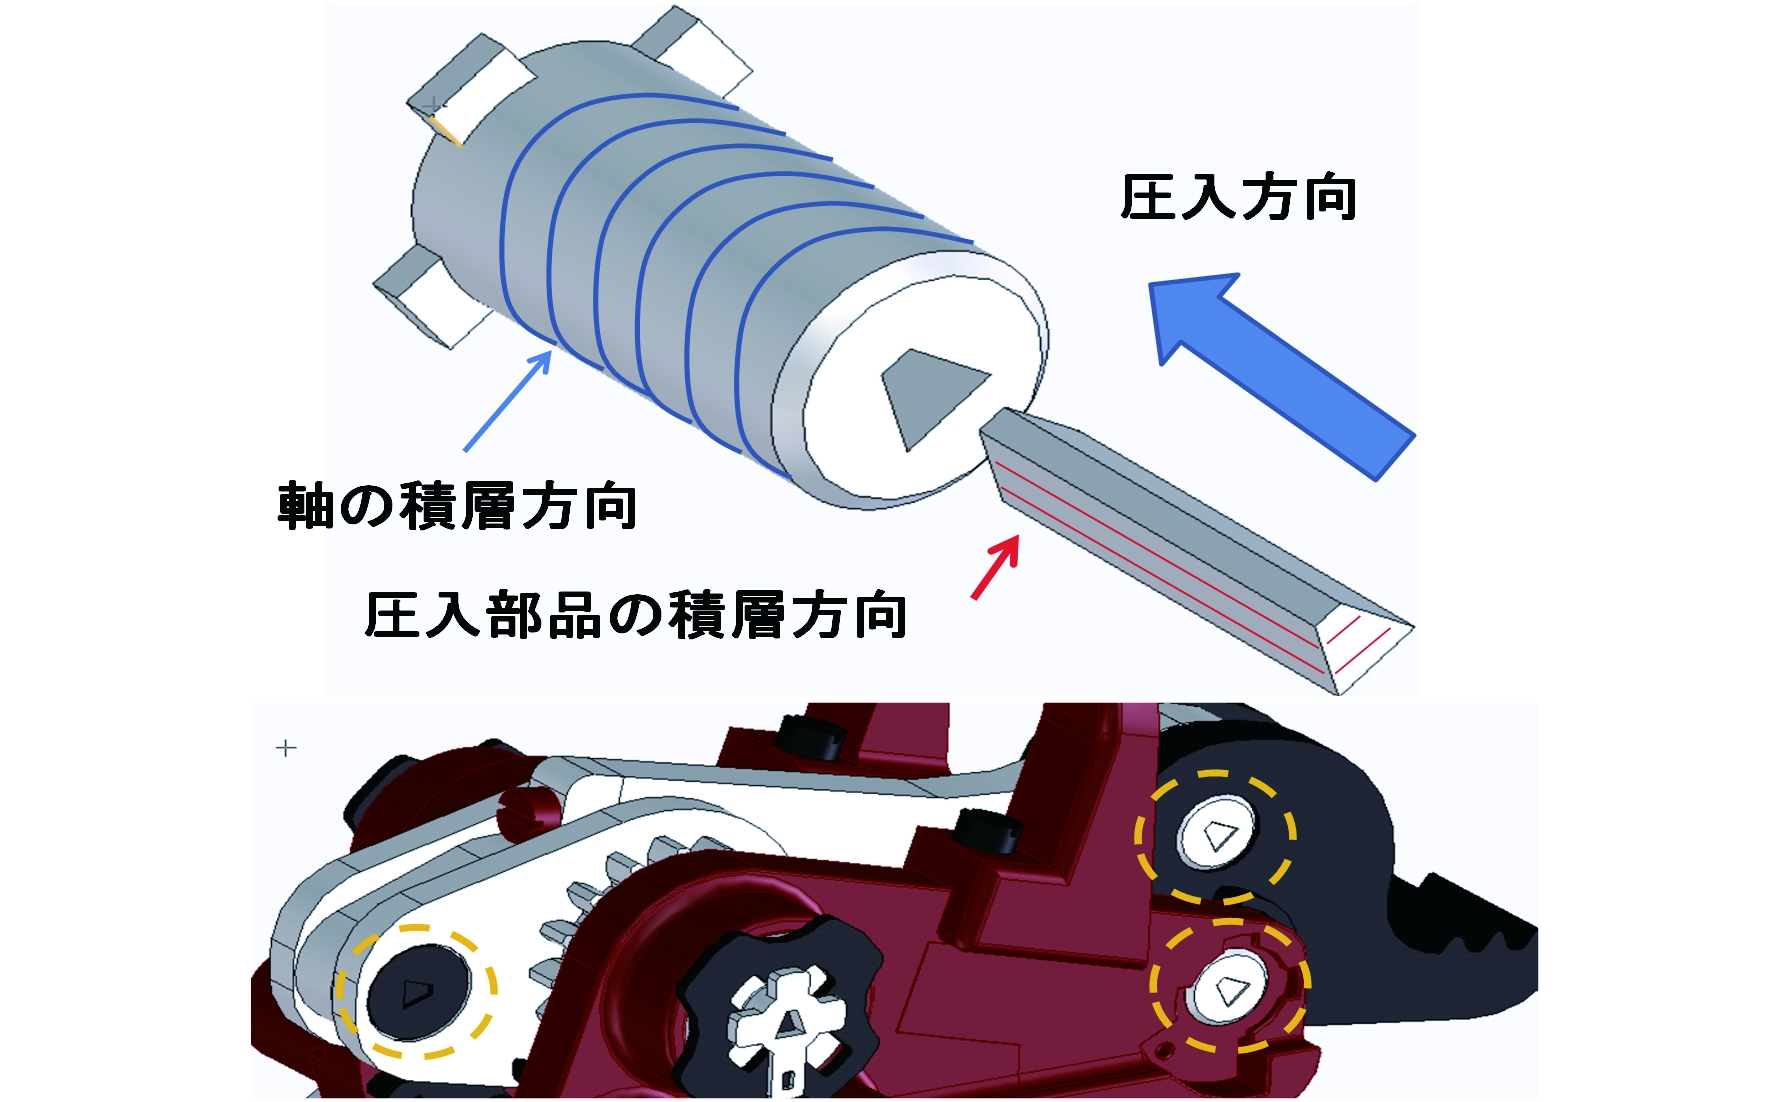
\includegraphics[width=370pt]{fig/fig20_cmyk.jpg}
\caption{積層方向の割れ防止構成}
\label{fig20}
\end{figure}

\clearpage

\section{モータ出力部の削れ防止構成}\label{ux30e2ux30fcux30bfux51faux529bux90e8ux306eux524aux308cux9632ux6b62ux69cbux6210}

ギアドモータ出力部には削れ防止構成を採用して設計しました。
モータ出力部から、3Dプリンタで製作した部品を、アルミ製の駆動伝達部品を介して接続しています。(Fig.\ref{fig19})

\begin{figure}[htbp]
\centering
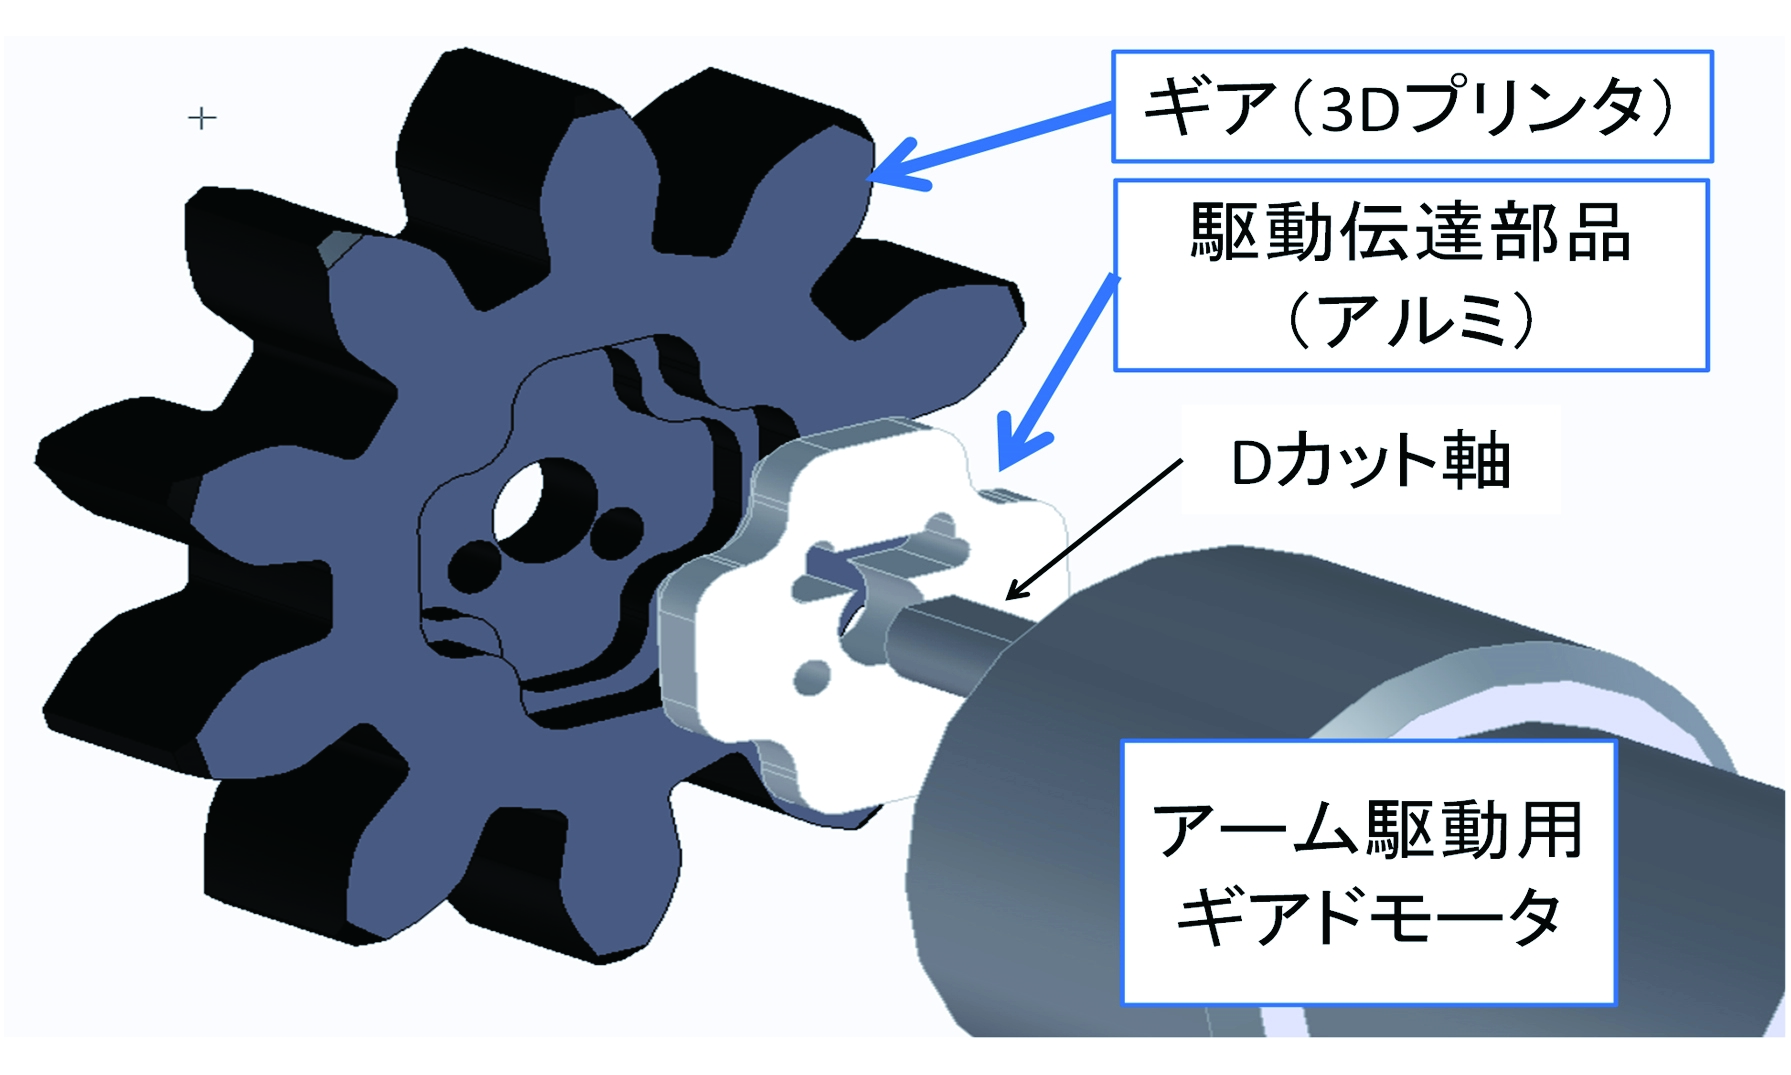
\includegraphics[width=190pt]{fig/fig19_cmyk.jpg}
\caption{モータ出力部の削れ防止構成}
\label{fig19}
\end{figure}

\section{大型部品の作成方法}\label{ux5927ux578bux90e8ux54c1ux306eux4f5cux6210ux65b9ux6cd5}

3Dプリンタのテーブルサイズを超える部品に関しては、分割・結合する必要があります。
本機体では、側面フレームが該当するため、2分割構成としました。
分割した部品同士の結合部に関しては断面形状を六角形とすることで、組立方向以外の方向に力がかかっても外れないようになっています。
また、組立方向を中間フレームに対して傾けることで、側面フレームを中間フレームに結合した後、組立方向に対する外れを防止しています。
(Fig.\ref{fig21})

\begin{figure}[htbp]
\centering
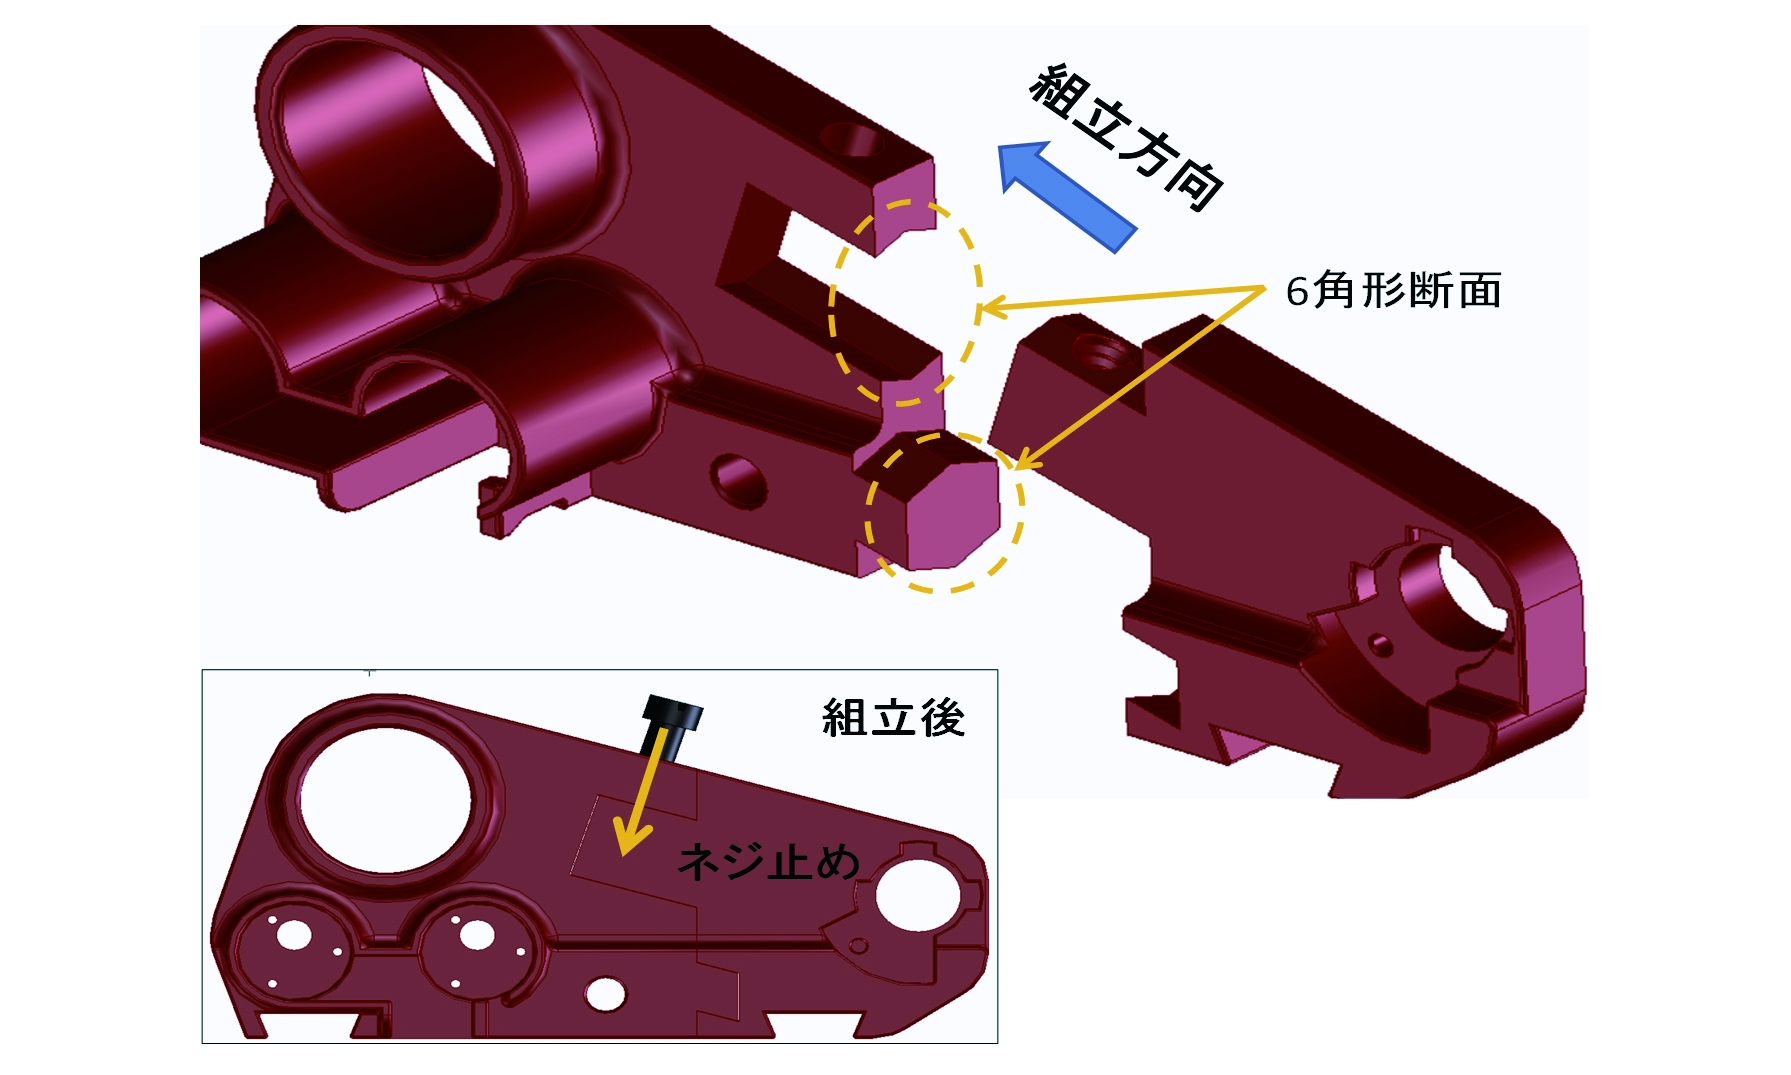
\includegraphics[width=290pt]{fig/fig21_cmyk.jpg}
\caption{大型部品の作成方法}
\label{fig21}
\end{figure}



\begin{thebibliography}{20}
\bibitem{ninjaflex}NINJAFLEX \\ \url{https://ninjatek.com/products/filaments/ninjaflex/}
\bibitem{tough-pla}TOUGH PLA \\ \url{https://www.makerbot.com/filament/tough-pla/}
\bibitem{kawasaki_public_HP}かわさきロボット競技大会 公式HP \\ \url{http://www.kawasaki-net.ne.jp/robo/}
\bibitem{creo_elements}PTC Creo Elements/Direct Modeling \\ \url{http://ja.ptc.com/product/creo/elements/direct-modeling}
\bibitem{tamiya_380k}タミヤ ギアドモータ380K \\ \url{http://www.tamiya.com/japan/robocon/robo_parts/g_motor/g_motor_zumen.htm}
\bibitem{replicator2x}Makerbot Replicator 2X \\ \url{http://makerbot.co.jp/contents/replicator2x.html}
\bibitem{pat01}日本特許 :小玉秀男. 立体図形作成装置. 特開昭56-144478. 1981-11-10. 
\bibitem{pat02}米国特許 : S. Scott Crump. Apparatus and method for creating three-dimensional objects. U. S. Patent 5121329 A. 1992-6-9. \\ \url{http://www.google.ca/patents/US5121329}
\bibitem{pat03}米国特許 : William J. Swanson. High temperature modeling apparatus. U. S. Patent 6722872 B1. 2004-4-20.	\\ \url{https://www.google.com/patents/US6722872}

\end{thebibliography}
\thispagestyle{empty}  
%------------------------------------------------------------------
%\appendix % 付録

%------------------------------------------------------------------
\backmatter % 後書きの開始
\chapter{おわりに}
\thispagestyle{empty} 

1980年、日本の小玉氏が光硬化樹脂を用いた「立体図形作成装置」の特許\cite{pat01}を出願しました。
これが3Dプリンタの元祖と言われています。
残念ながら製品化には繋がりませんでしたが、この時から光造形に関する特許が世界各国で出願されるようになりました。
そして1989年、米国Stratasys社が「Apparatus and method for creating three-dimensional objects」に関する特許\cite{pat02}を出願しました。
熱溶解積層法(FDM)3Dプリンタの基本特許です。2009年にこの特許権が失効したことから、世界各国3Dプリンタが発売されるようになりました。

私がこれを知って思ったのは、3Dプリンタは革新的な技術が産まれてできた製品ではないんだなぁ、ということです。
今はメイカーが増えたことで続々と関連技術が産まれているのでしょうが、そもそもの3Dプリンタは新しい技術で作られているわけではありません。

知られていないだけで、世の中にはまだまだ良い技術が眠っていそうです。
モノづくりがしやすくなった時代ですし、世界中から情報かき集めたら何か楽しいことができるのかも……
また何かネタを見つけたらこうして本にするのも面白いかもしれませんね。\\
最後まで読んでいただきありがとうございました。

\section*{発行}
でし・ぷろんぷと \\
2016年12月29日 第1版 発行

\section*{著者}
kyo46

\section*{Web} 
http://deshi-prompt.github.io/

\section*{Mail}
ada.robo1@gmail.com             

   

\newpage 
\pagestyle{empty}
%\printindex
%
%
\end{document}